%&pdflatex
%
%
%
%

% \documentclass[12pt]{article}
\documentclass[preprint,12pt]{elsarticle}

\usepackage{graphicx}
\usepackage{bm}
\usepackage{natbib}
\usepackage{xspace} % Incorporates correct optional space after commands
\usepackage{hyperref}

% Add line numbers
\usepackage[mathlines]{lineno} % Control line numbers

% Multipart figures
\usepackage{subcaption}  % "Newest" subfigure like package

% \oddsidemargin 0in
% \evensidemargin 0in
% \textwidth= 6.5in
% \topmargin -0.50in
% \textheight 9in

\usepackage{ifpdf} % For declaring rules for graphics below

\usepackage{latexsym,amssymb,amsmath,color}
\newcommand{\revised}[1]{\textcolor{blue}{{#1}}}
\newcommand{\comment}[1]{\textcolor{red}{{#1}}}
\newcommand{\alert}[1]{\textbf{\textcolor{red}{{#1}}}}
\newcommand{\be}{\begin{equation}}
\newcommand{\ee}{\end{equation}}
\newcommand{\xxi}{\vec{\xi}}
\newcommand{\xxii}{\xxi^{(\scriptscriptstyle{-}\scriptstyle{i})}}
\newcommand{\var}[1]{{\mathrm{Var}}\left[ {#1} \right]}
\newcommand{\ip}[2]{\left( {#1}, {#2} \right)}
\newcommand{\U}{\mathcal{U}}
\newcommand{\normim}[1]{\left\| {#1} \right\|_{\scriptscriptstyle L^{2}(\Omega^{*})}}
\newcommand{\avemu}[1]{\mathrm{E}\left({#1}\right)}
\newcommand{\ave}[1]{\left\langle {#1} \right\rangle}
\newcommand{\prob}[1]{\mathrm{Prob}\left\{ {#1} \right\}}
\newcommand{\ind}[1]{\mathrm{\chi}_{\scriptscriptstyle {#1} }}
\newcommand{\NISP}{\mathcal{S}}
\newcommand{\ipmu}[2]{\left( {#1}, {#2} \right)_\mu}
\newcommand{\norm}[1]{\left\| {#1} \right\|_{\scriptscriptstyle L^{2}(\Omega)}}
\newcommand{\pard}[2]{\frac{\partial{#1}}{\partial{#2}}}
\def\xbold{{\vec{x}}}
\renewcommand{\vec}[1]{{\mathchoice
                     {\mbox{\boldmath$\displaystyle{#1}$}}
                     {\mbox{\boldmath$\textstyle{#1}$}}
                     {\mbox{\boldmath$\scriptstyle{#1}$}}
                     {\mbox{\boldmath$\scriptscriptstyle{#1}$}}}}

\newcommand{\pd}{\pard}
\newcommand{\geoclaw}{{\sc GeoClaw}\xspace}
\newcommand{\tohoku}{T\={o}hoku\xspace}
\newcommand{\dx}{\ensuremath{\Delta x}}   % Delta x
\newcommand{\dy}{\ensuremath{\Delta y}}   % Delta y
\newcommand{\dt}{\ensuremath{\Delta t}}   % Delta t
        
\journal{Ocean Modelling}

\begin{document}

\ifpdf
\DeclareGraphicsExtensions{.pdf, .png, .jpg, .tif}
\else
\DeclareGraphicsExtensions{.png, .jpg, .tif, .eps}
\fi

\begin{frontmatter}

\title{Uncertainty Quantification and Inference of Manning's Friction Coefficient using DART Buoys Data during
\tohoku Tsunami}
\date{\today}

\author[kaust1]{Ihab Sraj}
\author[ut]{Kyle T. Mandli}
% \ead{kyle@ices.utexas.edu}
% \ead[http://users.ices.utexas.edu/~kyle]{http://users.ices.utexas.edu/~kyle}
\author[duke,kaust2]{Omar M. Knio}
\author[ut]{Clint N. Dawson}
\author[kaust]{Ibrahim Hoteit}
\ead{ibrahim.hoteit@kaust.edu.sa}
\ead{Division of Physical Sciences and Engineering, King Abdullah University for Science and Technology, Thuwal, Saudi Arabia}
\address[kaust1]{Division of Physical Sciences and Engineering, King Abdullah University for Science and Technology, Thuwal, Saudi Arabia}

\address[ut]{Institute for Computational Engineering and Science, University of Texas at Austin, 201 E 24th ST. Stop C0200, Austin, TX 78712-1229, USA}
\address[duke]{Department of Mechanical Engineering and Materials Science, Duke University, 144
Hudson Hall, Durham, North Carolina 27708, USA}
\address[kaust2]{Division of Computer, Electrical and Mathematical Sciences and Engineering, King Abdullah University for Science and Technology, Thuwal, Saudi Arabia}
\date{\today}

\begin{abstract}

Tsunami computational models are employed to explore multiple
scenarios and to predict water elevations.  However, accurate estimation of
water elevations  requires accurate estimation of many model parameters, in
particular the Manning's $n$ friction coefficient.  Our objective here is to
develop an efficient approach for the  uncertainty quantification and inference
of the Manning's $n$ coefficient which we characterize here by three different
parameters as being constant over three different regions: $n_1$ on-shore,
$n_2$ near-shore and $n_3$ deep-water.  We use Polynomial Chaos (PC) to build an
inexpensive surrogate for the  \geoclaw model and then employ Bayesian inference
to estimate  and quantify the uncertainties to those uncertain parameters using
the DART buoy data collected during the \tohoku tsunami.  The surrogate model
significantly reduces the computational burden of the Markov Chain Monte-Carlo
(MCMC)  sampling of the Bayesian inference. The PC surrogate is also used to
perform a sensitivity analysis.  Our results indicate that Manning's $n$
coefficients have a Maximum-A-Posteriori (MAP) values of $n_2=0.011$ and
$n_3=0.180$, while for $n_1$ no meaningful MAP value can be determined from the
available data.

\end{abstract}

\begin{keyword}
tsunami \sep Manning's $n$ friction coefficient \sep sensitivity analysis \sep polynomial chaos \sep Bayesian inference
\end{keyword}

\end{frontmatter}
\linenumbers

% \renewcommand{\thefootnote}{\fnsymbol{footnote}}

\begin{center}
\begin{Large}
{\bf Polynomial Chaos for the Estimation of Manning's Friction}\\

\end{Large}
\bigskip
\bigskip
Ihab Sraj$^1$, Kyle Mandli$^2$, Ibrahim Hoteit$^1$, \& Clint Dawson$^2$\\
\bigskip
$^1$Department of Physical Sciences and Engineering,
King Abdullah University for Science and Technology, Thuwal, Saudi Arabia \\
$^2$Institute for Computational Engineering and Science\\
University of Texas at Austin\\
Austin, TX 
\end{center}

\vspace{5.5cm}

\begin{tabbing}
Corresponding Author: \hspace{5mm} \=  \\
       \> Department of Physical Sciences and Engineering \\
       \> King Abdullah University for Science and Technology \\
       \> Thuwal, Saudi Arabia\\
       \> \\
Phone: \>  \\
Fax:   \>  \\
Email: \>    \\
\\
Submitted to: \> {\it TBD} \\
\> \today \\
\\
Revised: \>  

\end{tabbing}





% \clearpage

%!TEX root = paper.tex

\section{Introduction}

Tsunamis in the past decade have been responsible for some of the most 
deadly and costly natural disasters ever recorded. Coastal communities 
have faced this hazard by assessing the risk of these hazards, attempting 
to make informed decisions about the likelihood that such an event would 
occur with cost to life and property.  To do this, computational models of 
tsunami events are often employed to explore multiple different scenarios
to predict the water elevation caused by the tsunamis. The accurate prediction 
of water elevations requires accurate estimation of many model parameters that 
are either measured directly, defined empirically, or inferred from
sparsely collected data. Unfortunately, since tsunami events are relatively rare, 
there is an abundance of uncertainty in the input data for these computational 
models ranging from effects of the domain such as bathymetry and friction parameterizations, 
to the earthquake source.  In this article, we aim to estimate the Manning's n friction
coefficient that plays a key role in predicting the water elevation. 
Our approach is to quantify the uncertainty in the predicted water elevation 
and employ an inverse modeling approach to estimate the Manning's n coefficient 
using real observations of water elevation measured during the \tohoku tsunami as a case study.

Previous work looking into uncertainty in the input for tsunami simulations often has focused on the earthquake source but mainly as a way of constraining the various proposed earthquake scenarios only after the event (see for example \cite{MacInnes:2013cr}).  For instance, Sarri \emph{et al.} recently built a statistical surrogate of a landslide-generated tsunami computer model by using an emulator~\cite{Sarri2012}. The implemented emulator was the Gaussian process that requires using a combination of prior knowledge about the simulator and
appropriate choices of functions and parameters. Their work was presented as a proof-of-concept case study
where they performed basic statistical and sensitivity analysis. In this work we focus on the uncertainty in the friction parameterization used in tsunami simulations.  Changes to the friction parameterization has been shown in the past to lead to significant changes to inundation levels \cite{Myers:2001el,Jakeman:2010hk} but these previous studies were limited in the scope of the changes allowed.  In a recent work, Mayo et el. reformulated a statistical data assimilation method generally used in the estimation of model states to estimate Manning's n coefficient~\cite{Mayo2013}. They used a low-dimensional representations of Manning's n coefficients and recovered it by assimilating water elevation data.

In this work, we aim at making use of the recent developments in Uncertainty Quantification 
(UQ) methods that allows probing the sensitivity of realistic tsunami models 
to uncertain parameters, and inferring those parameters from specific observations. 
In particular, we implement an inverse modeling approach that relied on the Bayesian inference approach.  
We will also rely on Polynomial Chaos (PC) expansions to construct a 
faithful surrogate of the response of the large and complex geophysical 
model simulations.  The construction of the surrogate enables us to efficiently 
implement the Bayesian inference formalism as it dramatically reduces the cost of 
sampling the posterior distribution. 

PC expansions have been developed and applied in the engineering community to quantify uncertainties
in numerical simulations; their principal use is in propagating input
uncertainties through large, complex and non-linear models to compute the
ensuing output uncertainties. Several researchers have been 
investigating the applicability of PC expansions for UQ in oceanic simulations
\citep{thacker2012,ashwanth2010,Alexanderian2012}. Recently,
PC combined with Bayesian inference was used to estimate drag coefficient
during Typhoon Fanapi 2010. The same problem was solved using
the adjoint method and MCMC \cite{sraj:2013a,sraj:2013b}.

In this work, we follow a similar procedure as in \cite{sraj:2013a,sraj:2013b}
to estimate Manning'n n coefficient of friction. 
%We use the widely used Manning's n law to provide a relationship between the friction coefficient and the roughness parameter $n$.  The parameter $n$ is also allowed to vary in space determined by the initial water depth to study effects of deep-water, near-shore, and on-shore sensitivities.  
To carry out the uncertainty quantification we have employed polynomial chaos expansions.  Here the quantity of interest is taken to be the surface elevation $\eta$ and will compared to available NOAA Deep-ocean Assessment and Reporting of Tsunamis (DART) buoys for the \tohoku tsunami.  The forward model runs are performed using \geoclaw following the setup and using one of the source models explored in \cite{MacInnes:2013cr}.

\alert{maybe an outline for this paper}

%!TEX root = paper.tex

\section{The \tohoku Tsunami} 
\label{sec:tohoku}

The \tohoku earthquake and tsunami of 2011 has been the subject of a number of studies due to the wealth of observational evidence and severity of the tsunami.  The earthquake itself had an estimated magnitude of $\text{M}_\text{w}$ 9.0 and caused massive devastation across Japan.  In the case study presented, the simulation is based on work done in \cite{MacInnes:2013cr} and modified to use the specified variable friction field.
In this section we briefly describe the forward computational model used, \geoclaw, and the 
simulation setup used in the uncertainty analysis and finally describe
the observations from NOAA DART buoys.

%\section{Simulation Setup}
%\label{sec:simulation}


\subsection{\geoclaw} \label{ssub:geoclaw}

The \geoclaw software package uses a finite volume, wave-propagation approach described in \cite{LeVeque:1997eg} to solve the two-dimensional shallow water equations:
\begin{equation} \label{eq:swe}
    \begin{aligned}
    &\pd{}{t} h + \pd{}{x} (hu) + \pd{}{y} (hv) = 0, \\
    &\pd{}{t}(hu) + \pd{}{x} \left(hu^2 + \frac{1}{2} g h^2 \right ) + \pd{}{y} (huv) = ~~ fhv - gh \pd{}{x} b - C_f |\vec{u}| hu \\
    &\pd{}{t} (hv) + \pd{}{x} (huv) + \pd{}{y} \left (hv^2 + \frac{1}{2} gh^2 \right) = -fhu - gh \pd{}{y} b - C_f |\vec{u}| hv
    \end{aligned}
\end{equation}
where $h$ is the depth of the water column, $u$ and $v$ the velocities in the 
longitudinal and latitudinal directions respectively, $g$ the acceleration due 
to gravity, $b$ the bathymetry, $f$ the Coriolis parameter, and $C_f$ the bottom 
friction coefficient.  As is common in tsunami modeling, $C_f$ is calculated 
given a Manning's $n$ parameterization such that:
\begin{equation}
    C_f = \frac{g n^2}{h^{5/3}}
\label{eq:coef}
\end{equation}
where $n$ is an empirically determined parameter known as Manning's $n$.  

The primary computational kernel in \geoclaw is the evaluation of the solution to the Riemann problem at each grid cell interface.  The Riemann solver used includes the ability to handle inundation (wet-dry interfaces), well-balancing, even when the momentum is non-zero, and entropy corrections \cite{George:2008aa}.

\subsubsection{Adaptivity} \label{ssub:adaptivity}
One unique feature that \geoclaw has is the ability to adaptively refine the grids used for the computation essentially following a region of interest as time progresses (in this case, the disturbance in the surface height $\eta$).  \geoclaw implements these algorithms following \cite{Berger:1984ui,Berger:1998aa} and is described in detail in \cite{Berger:2011du} in the case of tsunami modeling.

For the simulations presented, refinement thresholds were used that matched what was presented in \cite{MacInnes:2013cr}.  As was done there, four levels of refinement were used staring with a resolution of 1 degree in both the latitudinal and longitudinal directions down to 0.5' resolution (approximately 900 meters) located around the observation locations.  The tolerance for the refinement criteria for sea-surface anomaly was 0.02 meters.

\subsection{The \tohoku Tsunami} \label{ssub:tohoku}

The \tohoku earthquake and tsunami of 2011 has been the subject of a number of studies due to the wealth of observational evidence and severity of the tsunami.  The earthquake itself had an estimated magnitude of $\text{M}_\text{w}$ 9.0 and caused massive devastation across Japan.  In the case study presented, the simulation is based on work done in \cite{MacInnes:2013cr} and modified to use the specified variable friction field.

\subsection{Source Model and Bathymetry}

The MacInnes \emph{et al.} study found that source models from tsunami
inversions were 

Since the previous study \cite{MacInnes:2013cr} did not find that the source model effected the tsunami wave-forms at the DART buoys, we did not expect there to be much difference between the available models.  After comparing the same analysis with two different source models, namely the models from \cite{Ammon:2011dm} and .

[4] Ammon used a seismic and GPS inversion technique
[7] Saito et al. used a tsunami inversion

Since the previous study found that the source model used did not impact the off-shore gauge stations, the ones used here from \cite{Ammon:2011dm}, was chose the source model that was commonly available.  Access to the finest bathymetry located near the Japanese coastline was also not included as it primarily effected only the shore observations.
\comment{The bathymetry is shown in Figure~\ref{fig:setup} in addition to the topography
of the Pacific Ocean.}

<<<<<<< HEAD
\subsubsection{Bathymetry}
The bathymetry used in the simulation is a combination of ETOPO 1' and 4' 
accurate bathymetry for the region \cite{Amante:2009ud}.  The additional 
bathymetry data used in the MacInnes \emph{et al.} was useful only near the
shore and had a smaller effect on the regions near the observations used in
this study.  

\subsubsection{Observations}
The observations used in this study are from the Deep-ocean Assessment and Reporting of Tsunamis (DART) buoy system developed and maintained by the National Oceanic and Atmospheric Administration (NOAA).  The purpose of the network is to provide early-warning detection and forecasting of tsunami propagation in the Pacific Ocean \alert{need citation for this?}.  The DART buoys closest to the earthquake source of the \tohoku tsunami were buoys 21401, 21413, 21418, and 21419 whose locations are shown in Figure~\ref{fig:setup}(left) and whose de-tided data for the event are shown in Figure~\ref{fig:setup}(right).

\subsection{DART Buoys Observations}

The observations used in this study are from the Deep-ocean Assessment and Reporting of Tsunamis (DART) buoy system developed and maintained by the National Oceanic and Atmospheric Administration (NOAA).  The purpose of the network is to provide early-warning detection and forecasting of tsunami propagation in the Pacific Ocean \alert{need citation for this?}.  The DART buoys closest to the earthquake source of the \tohoku tsunami were buoys 21401, 21413, 21418, and 21419 whose locations are shown in Figure~\ref{fig:setup}(left) and whose de-tided data for the event are shown in Figure~\ref{fig:setup}(right). \comment{maybe more description of the data in the figure}.



\section{Manning’s $n$ Friction Parameterization}
%We use the widely used .  The parameter $n$ is also allowed to vary in space determined by the initial water depth to study effects of deep-water, near-shore, and on-shore sensitivities.  

Manning's $n$ law provides a relationship between the friction coefficient appearing in the shallow
water equations governing tsunamis and the roughness parameter $n$. 
This Manning's $n$ coefficient is variable that is highly spatial 
and dependent on the surface characteristics of the sea-floor. 
The direct measurement of $n$ is therefore impossible, instead, values
are often assigned from tables that are empirically estimated
for common types of land that are determined from satellite images.
As a result, the Manning’s n coefficients used in tsunami models
often contain large amounts of uncertainty.

The uncertainty in the Manning's $n$ coefficient leads to uncertainties
in the predicted quantities of interest such as the water elevations
and becomes a health risk during tsunami events. In addition, 
the prediction of these quantities of interest are often highly sensitive to 
the changes in these uncertain parameters. 
In this work, we seek to quantify parametric uncertainty namely due 
to the uncertainty in the roughness parameter $n$. To this end,
we characterize the roughness $n$ by three different parameters
that are varied in three different regions but are assumed
constant in each region. The three regions are as follows: 
on-shore whose coefficient is denoted by $n_1$, near-shore 
denoted by $n_2$, and deep-water denoted by $n_3$.
The three regions are shown in Figure~\ref{fig:ceofs}.
To carry out the uncertainty quantification we have employed polynomial chaos expansions 
as used in \cite{sraj:2013a,sraj:2013b}. The method and its application
to our problem is described in Section~\ref{sec:uqpce}.  
To represent the uncertainty in the Manning's $n$ coefficients a uniform distribution was assumed as the prior where $N$ was sampled in the interval $n \in [0.005-0.2]$.  

Note that on the Sendai plain a Manning's $n$ value of 0.035 was used to account for pasture, farmland and rice paddies.

\section{Manning's Friction Coefficient} \label{sec:manning}

Manning's $n$ law provides a relationship between the friction coefficient 
(Equation \ref{eq:coef}) appearing in the shallow
water equations governing tsunamis (see Equation \ref{eq:swe})
and the roughness parameter $n$. 
This Manning's $n$ coefficient is variable that is highly spatial 
and dependent on the surface characteristics of the sea-floor. 
The direct measurement of $n$ is therefore impossible, instead, values
are often assigned from tables that are empirically estimated
for common types of land that are determined from satellite images.
As a result, the Manning's $n$ coefficients used in tsunami models
often contain large amounts of uncertainty.

The uncertainty in the Manning's $n$ coefficient leads to uncertainties
in the predicted quantities of interest such as the water elevations
and becomes a health risk during tsunami events. In addition, 
the prediction of these quantities of interest are often highly sensitive to 
the changes in these uncertain parameters. 
In this work, we seek to quantify parametric uncertainty namely due 
to the uncertainty in the friction parameter $n$. To this end,
we characterize the Manning's $n$ coefficient by three different parameters
that are varied in three different regions but are assumed
constant in each region. The three regions are as follows: 
on-shore whose coefficient is denoted by $n_1$, near-shore 
denoted by $n_2$, and deep-water denoted by $n_3$.
The three regions are shown in Figure~\ref{fig:ceofs}.
To carry out the uncertainty quantification we have employed polynomial chaos expansions 
as used in \cite{sraj:2013a,sraj:2013b}. The method and its application
to our problem is described in Section~\ref{sec:uqpce}.  
To represent the uncertainty in the Manning's $n$ coefficients a uniform 
distribution was assumed as the prior where $n$ was sampled in the interval $n \in [0.005,0.2]$.  


\section{Formulation}
\label{sec:formu}
In this section, we first present the Bayesian approach to inverse problems 
and its application to our problem of inferring the Manning's $n$ coefficients.
We also introduce
a Polynomial Chaos method used for forward uncertainty propagation, and 
for accelerating the Bayesian inference based on the resulting surrogate.

\subsection{Bayesian Inference}
 \label{sec:inference}
 
Bayesian inference is a statistical approach to inverse problems
that has recently gained great interest in different applications, including
ocean~\citep{Alexanderian2011a,Zedler2012,sraj:2013a}
climate~\citep{OlsonEtAl2012} and geophysical~\citep{Malinverno2002} modeling.
The key idea in this approach is to express all forms of uncertainty
in terms of probability. The first step in Bayesian inference 
is to formulate the forward problem (response surface/model) using 
a suitable likelihood function and a product of conditional probability densities. 
The prior distributions over the unknown parameters of the model
are then formulated using the best available knowledge of the parameters.  Lastly, given some observation data, Bayes rule 
is used to obtain a posterior distribution for these unknown parameters
\citep{sivia}. We review this approach briefly below.
\subsubsection{Formalism}

Let $\vec{d}=(d_1,...,d_m)^T$ be a vector of observation data and $\vec{\theta}=(\theta_1,...,\theta_n)^T$ be a vector of model parameters or inputs. We consider a forward model $\vec G$ that predicts the data function of 
the parameters such that:

\begin{equation}
\vec d \approx \vec{G}( \vec \theta).
\end{equation}
Applying the Bayes' rule yields:

\begin{equation}
 \Pi(\vec{\theta}| \vec d) \propto 
 L(\vec d | \vec{\theta}) \ q(\vec{\theta}), 
\label{eq:bayes}
\end{equation}
where $q(\vec{\theta})$ is the prior of $\vec{\theta}$, representing the \emph{a priori} knowledge
about the parameters; 
$L(\vec d| \vec{\theta})$ is the likelihood function representing
the probability of obtaining the data given the set of parameters $\vec{\theta}$;
and finally $\Pi(\vec{\theta}| \vec d)$ is the posterior,
representing the probability of occurrence of $\vec{\theta}$ given the data $\vec d $.

To formulate the likelihood function, we let $\vec \epsilon = \vec d - \vec{G}$
represent the discrepancy between the model and observations.
Here, the components of $\vec \epsilon $ are assumed to be i.i.d. random variables with density $p_{\epsilon}$.
The likelihood function can thus be written as:

\begin{equation} 
L(\vec d |  \vec{\theta}) 
= 
\prod_{i=1}^m  
p_\epsilon (d_i - G_i(\vec \theta)).  	
\label{eq:likelihood}
\end{equation}

In our application, we assume that the errors $\epsilon_i$ are independent
and normally distributed with mean
zero and variance $\sigma^2$, i.e. $\epsilon_i \sim N(0,\sigma^2)$. 
While in general $\sigma^2$ (the variance of the noise in the measured data) depends on the observations, in our case we assume that the error
amplitude is generally small and does not change throughout space and time.
Consequently, one may assume a single $\sigma^2$ value in Equation~\eqref{eq:likelihood},
resulting in:

\begin{equation} 
L(\vec d |  \vec{\theta}) 
= 
\frac{1}{\sqrt{2 \pi \sigma^2}}\prod_{i=1}^m   
\exp \left\lbrace \frac{-(d_i - G_i(\vec \theta))^2}{2 \sigma^2} \right\rbrace. 	
\label{eq:likelihood2}
\end{equation}
The joint posterior from Bayes' rule can be given as:

\begin{equation} 
\Pi(\vec{\theta}| \vec d)
\propto
\frac{1}{\sqrt{2 \pi \sigma^2}}   \prod_{i=1}^m  
\exp \left\lbrace \frac{-(d_i - G_i(\vec \theta))^2}{2 \sigma^2} \right\rbrace  
\prod_{i=1}^n q(\theta_i).
\end{equation}
Since $\sigma^2$ is unknown \emph{a priori} we treat it as a hyper-parameter.
In other words, $\sigma^2$ becomes an additional parameter for Bayesian inference and  
therefore endowed with a prior which is updated based on available observations. In this 
case the joint posterior is finally expressed as:

\begin{equation} 
\Pi(\vec{\theta},\sigma^2 | \vec d)
\propto
\frac{1}{\sqrt{2 \pi \sigma^2}}   \prod_{i=1}^m  
\exp \left\lbrace \frac{-(d_i - G_i(\vec \theta))^2}{2 \sigma^2} \right\rbrace
\ q(\sigma^2) \prod_{i=1}^n q(\theta_i).
\label{eq:post}
\end{equation}


\subsection{Inferring Manning Friction Coefficient}
 \label{sec:manning}
 
We seek to infer the Manning coefficient from water surface elevation
data measured at different gauges as shown in Figure~\ref{fig:setup}.
Bayesian inference can be applied directly to infer the uncertain parameters
using Equation~\eqref{eq:post}. In our case, the observation data $\vec d$ 
are the water surface elevation at the gauges;
their model predicted counterparts $\vec G$ is predicted by \geoclaw.
The uncertain parameters $\vec \theta$ will be denoted by $\{N_i\}_{i=1}^3$ for the
three Manning Friction coefficients treated as the unknown parameters. 
In this case  Equation~\eqref{eq:post} can be written as:

\begin{equation} 
p(N_1,N_2,N_3,\sigma^2 | \vec d) 
\propto \frac{1}{\sqrt{2 \pi \sigma^2}} 
 \prod_{i=1}^m  
\exp \left\lbrace \frac{-(d_i - G_i)^2}{2 \sigma^2} \right\rbrace
\ p(\sigma^2)p(N_1)p(N_2) p(N_3)
\label{eq:post_coef}
\end{equation}

To complete the definition of the posterior, we need to choose a proper prior that should be based 
on some \emph{a priori} knowledge about the parameters. In our case, a uniform
prior for the model parameters is assumed as indicated:

\begin{equation} 
p(N_i) = \begin{cases}
		\displaystyle \frac{1}{b_i-a_i} &\text{for~} a_i <  N_i \leq b_i ,  \\
		0 &\text{otherwise}  , 
\end{cases}
\end{equation}
where $ [a_i,b_i]$ denote the parameter ranges defined as.
Regarding the variance, the only information we know 
is that $\sigma^2$ is always positive.
We thus assume a Jeffreys prior \citep{sivia}, expressed as:

\begin{equation} 
p(\sigma^2) =  \begin{cases}
		\displaystyle \frac{1}{\sigma^2} &\text{for~} \sigma^2 > 0,  \\
		0 &\text{otherwise}. 
		\end{cases}
\label{eq:var_pr}
\end{equation}

Inferring the coefficients requires 
sampling the posterior. In general, when the space of the unknown 
parameters is multidimensional, a suitable computational strategy is 
the Markov Chain Monte  Carlo (MCMC) method. 
We rely on an adaptive Metropolis MCMC \citep{Gareth2009,Haario2001} to
sample the posterior distribution accurately and efficiently.




%!TEX root = paper.tex
\subsection{Accelerating Bayesian Inference}
\label{sec:uqpce}

The four-dimensional posterior in Equation~\eqref{eq:post_coef} can be directly
explored via MCMC; this requires repeated simulations (tens of thousands) of the forward \geoclaw model, 
once for every proposed set of parameters of the Markov chain~\cite{MarzoukNajm2009,Malinverno2002}. 
While a single \geoclaw simulation takes about $15~$mins, depending on the details of the MCMC algorithm used, 
it is desirable to avoid running the forward model at every realization of the MCMC. 
This is achieved by constructing a surrogate model that requires a much
smaller ensemble of \geoclaw runs, and that can be used instead
at a significantly reduced computational cost.  Here, we rely on
Polynomial Chaos expansions for accelerating Bayesian inference in this context 
by building a surrogate model, which, in addition can efficiently
provide statistical properties, such as the mean, variance and sensitivities. 

\subsubsection{Polynomial Chaos}

Polynomial Chaos (PC) is a probabilistic methodology that expresses the 
dependencies of model outputs on the uncertain model inputs
as a polynomial truncated expansion~\citep{Villegas2012,Lin2009,Xiu2004}.
We briefly describe the PC method below; for more details 
the reader is referred to \citep{LeMaitreKnio2010}.

Let $U=U(\bm{x},t,\xxi)$ denote a quantity of 
interest (QoI) that is the output of a computational model.
$U$ is function of space, $\bm{x}$, and time, $t$, and 
also depends on the canonical vector of random variables $\xxi=(\xi_1,...,\xi_n)$
that parameterize the uncertain inputs. 
PC expresses $U$ in the form:

\begin{equation}
  U(\xbold,t,\xxi) \doteq \sum_{k = 0}^P U_k(\xbold,t) \Psi_k(\xxi),
\label{eq:stochseries}
\end{equation} 
where $U_k(\xbold,t)$ are the polynomial coefficients, and
$\Psi_k(\xxi)$ are functions that form an orthogonal basis of an underlying probability
space. The total number of terms in the PC expansion is
$P+1 = \frac{(d+p)! }{n!\ p!}$ where $n$ is the number of stochastic dimensions and $p$ is the highest order
polynomial order. 

The choice of the basis is dictated by the probability density
function of the stochastic variable $\xxi$, which appears as a weight
function in the probability space's inner product:

\begin{equation}
 \left<\Psi_i,\Psi_j\right> = \int \Psi_i(\xxi) \;\Psi_j(\xxi) \; \rho(\xxi) \; \mbox{d}\xxi=\delta_{ij}\ave{\Psi_i^2},
\label{eq:inner}
\end{equation}
where $\delta_{ij}$ is the Kronecker delta.
For uniform
distributions, the basis functions are scaled Legendre polynomials.
For multi-dimensional problems the basis functions are
tensor products of 1D basis functions~\cite{LeMaitreKnio2010}.

The series representation \eqref{eq:stochseries} can be viewed as a spectral expansion
of $U$ along the stochastic dimensions. It can also be seen as a
combination of approximation and probabilistic frameworks; this
 has proven extremely useful in solving UQ problems~\cite{Xiu:2003,Lin2009}. The existence and convergence of this series is asserted by the Cameron-Martin theorem \citep{Cameron:1947} with the condition that $U$ has a finite variance.
The series rate of convergence, and hence the number of terms to retain, depends on the smoothness of
$U$ with respect to $\xxi$. The series converges spectrally fast with $P$
when $U$ is smooth; the convergence rate becomes algebraic
when $U$ has finite smoothness \citep{Canuto:2006}. In practice the series convergence is monitored 
via various error metrics as discussed in the results section.

\subsubsection{Non Intrusive Spectral Projection (NISP)}
The computation of the coefficients of the PC expansions $U_k$
can be done using a number of procedures. Here we adopt a non-intrusive
approach that allows the use of the forward model \geoclaw as a black box
with no code modifications required. PC expansion coefficients are determined
based on a set of response \geoclaw simulations at a specified set of the uncertain parameters. 
Specifically, we rely on the Non-Intrusive Spectral Projection (NISP) method that exploits the orthogonality of the basis and applies the Galerkin projection to find the PC expansion coefficients as follows:

\begin{equation}
 U_k(\bm{x},t) = \frac{\left< U, \Psi_k \right>}{\left< \Psi_k, \Psi_k \right>} = 
 \frac{1}{\left< \Psi_k, \Psi_k \right>} 
 \int U(\bm{x},t,\xxi) \Psi_k(\xxi) \rho(\xxi) \mbox{ d}\xxi.
\end{equation}
This orthogonal projection minimizes the $L_2$ error on the space spanned by the basis.
Using NISP the stochastic integrals are solved using a numerical quadrature to obtain:

\begin{equation}
  \left< U, \Psi_k \right> 
\approx \left< U, \Psi_k \right>_Q
= \sum_{q=1}^Q U(\xxi_q) \Psi_k(\xxi_q) \omega_q,
\end{equation}
where the subscript $Q$ refers to approximating the inner product integral with
quadrature, and $\xxi_q$ and $\omega_q$ are multi-dimensional quadrature points and weights,
respectively. The quadrature order should be commensurate with the
truncation order, and should be high enough to avoid aliasing artifacts.
The choice of quadrature rule is hence critical to the performance
of the PC (in its NISP version at least).

The computation of the ${U}_k$ can thus be expressed as a matrix-vector product of the form:

\begin{equation} 
 U_k(\bm{x},t)=\sum_q \Pi_{kq} U(\bm{x},t,\xxi_q),\;\;\;
 \Pi_{kq}=\frac{\Psi_k(\xxi_q)\omega_q}{\left< \Psi_k, \Psi_k \right>},
\label{eq:nisp}
\end{equation} 
where $\Pi_{kq}$ is the projection matrix and $U(\bm{x},t,\xxi_q)$ is obtained
from an ensemble of the deterministic model realizations with the uncertain parameters set at
the quadrature value $\xxi_q$. 


\subsubsection{Statistical moments and sensitivity analysis}
The identification of the inner product weight function
with the probability distribution of $\xxi$ simplifies the calculations of the statistical moments of $U$. 
Noting that since $\Psi_0(\xxi)$ is a constant that is normalized so that 
$\left<\Psi_0,\Psi_0\right>=1$, the expectation and variance of $U$ can be computed as:

\begin{equation}
 E[U] = \int U \, \rho(\xxi) \, \mbox{d}\xxi=\left< U,\Psi_0\right> = U_0,  
 \label{eq:mean}
\end{equation}
and \begin{equation}
 E[(U-E[U])^2] = \int (U-E[U])^2 \, \rho(\xxi) \, \mbox{d}\xxi=\sum_{k=1}^P U_k^2
 \label{eq:sigma}
\left<\Psi_k,\Psi_k\right>.
\end{equation}

PC representations also enable
efficient global sensitivity analysis that quantify the
contributions of different random input parameters to the variance in the output.
This can be done by computing the so-called {\it total} 
sensitivity index $T_i$ that measures the contribution of
the $i^{th}$ random input to total model variability by
computing the fraction of the total variance due to all the terms in the
PC expansion that involve $\xi_i$~\citep{LeMaitreKnio2010,Crestaux,Sudret}
as follows:

% of random variables from the PC representations or Sobol decomposition~\citep{Sobol:1993,Homma:1996,Sobol:2001}. The total sensitivity index  
%
%To get the total sensitivity corresponding to the uncertain
%input $\xi_i$ we compute the total index:

\begin{equation} \label{eq:T-hard}
   T_i =
         \frac{\displaystyle
               \sum_{k \in K_i} U_k^2 \ave{\Psi_k^2}}
              {\displaystyle\sum_{k = 1}^P U_k^2 \ave{\Psi_k^2}},
\end{equation}
where \[
   K_i = \left\{ k \in \{1, \ldots, P\} :
           \vec{\alpha}^k_i > 0 \right\},
        \]
and $\vec{\alpha}^k$ is the multi-index associated with the $k^{th}$ term in the
PC expansion~\cite{LeMaitreKnio2010}.

%Using Equation~\eqref{eq:T-hard}, the computation of $T_i$ is straightforward.





\section{Results}
\label{sec:results}
We begin the results section by performing
an error and convergence analysis of the
constructed surrogate using the PC expansions
to establish its validity in Section~\ref{sec:analysis}.
Then in Section~\ref{sec:forward}, we present
statistical analysis to quantify the uncertainty in the predicted surface elevation
as well as a sensitivity analysis to rank the impact of the different Manning's 
roughness coefficients on this uncertainty. 
Finally, in Section~\ref{sec:inverse}, we present the results of the inverse
problem where we determined the posterior distributions of the input parameters 
and analyzed them in light of the available gauge data.
\subsection{Error and convergence study}
\label{sec:analysis}

Figure~\ref{fig:rlzs} shows the evolution of the
water surface elevation for the 125 realizations obtained 
to compute the PC expansions at the four different gauge 
locations. We notice that the variation in surface elevation 
is negligible during the first hour at gauge number 21418 
and during the first two hours for the remaining gauges
as the plots of the different realizations are seen to superimpose.
However, a noticeable uncertainty in the surface 
elevation can be seen  at all gauges as indicated from the thickness 
of the bands formed by the plots of the realizations. This uncertainty
occurs till the end of the simulations.
\begin{figure}[h]
\centering
\begin{tabular}{clc}        
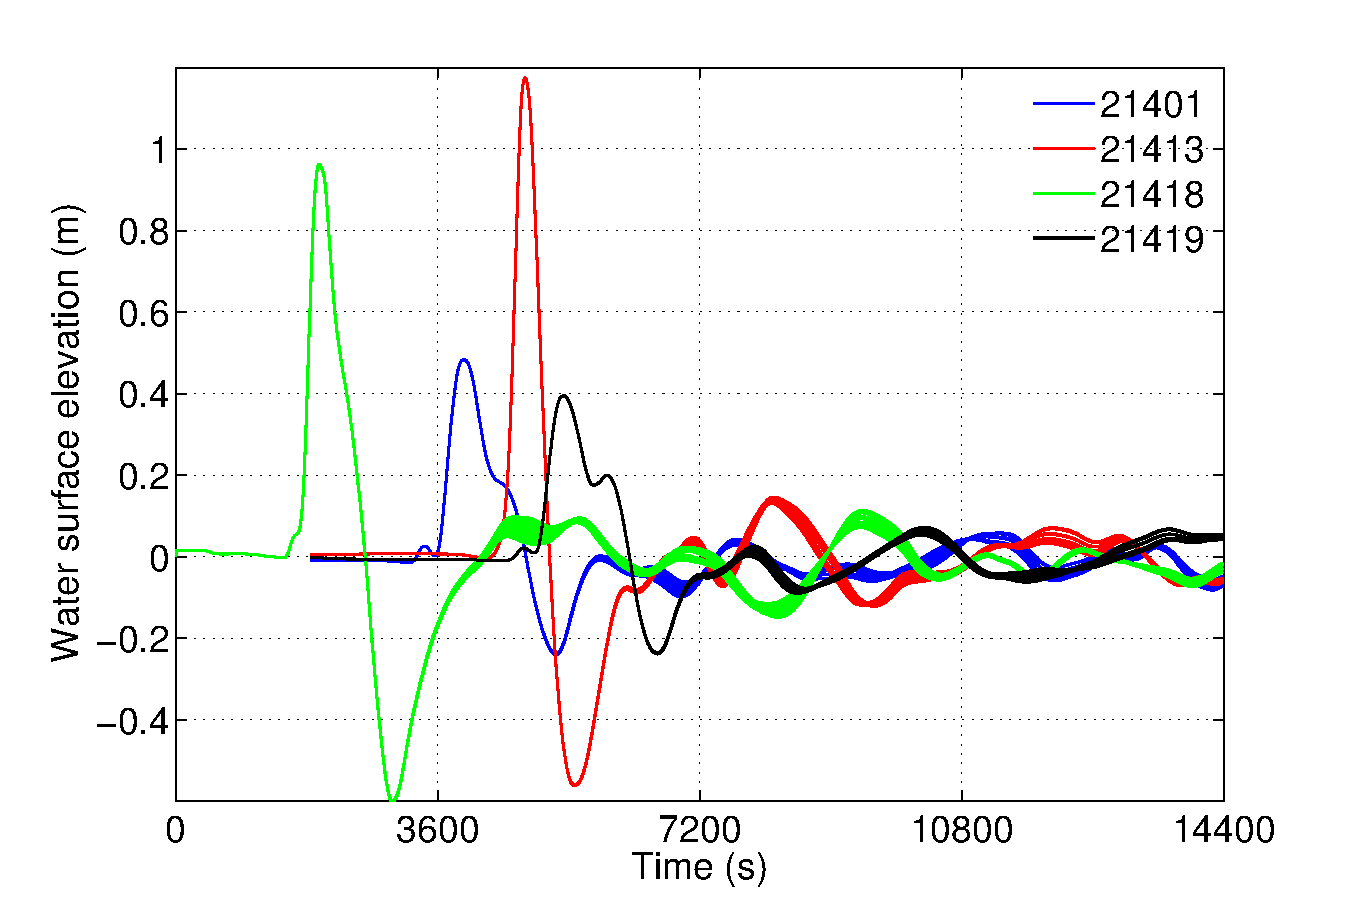
\includegraphics[width=0.6\textwidth]{figures/rlzs_gauges.pdf} 
\end{tabular}
\caption{125 Geoclaw realizations at different gauge locations.}
\label{fig:rlzs}
\end{figure}


In order to check the consistency of the approximation, we compare
 water surface elevation from the realizations 
with those obtained from the PC surrogate. The different curves
show an excellent agreement (not shown) for all times. We also define
an error metric that measures the relative normalized root mean-square error between the left hand side function 
in Equation~(\ref{eq:stochseries})
and its PC representation at the sampling points:
\begin{equation} 
   E = \frac{\displaystyle
         \left(\sum_{\xxi \in \NISP} \left|U(\xxi) - \sum_{k = 0}^{P}
U_k\Psi_k(\xxi)\right|^2
         \right)^{1/2}}
        {\displaystyle
          \left(\sum_{\xxi \in \NISP} \left|U(\xxi)\right|^2\right)^{1/2} 
          },
\label{eq:error}
\end{equation}
where $\NISP$ is the 125-member ensemble obtained using the PC algorithm. 
This error metric calculated at the different gauge locations is shown in Figure~\ref{fig:error};
the largest relative normalized error for 
water surface elevation is about 0.1\% . 
\begin{figure}[h]
\centering
\begin{tabular}{clc}        
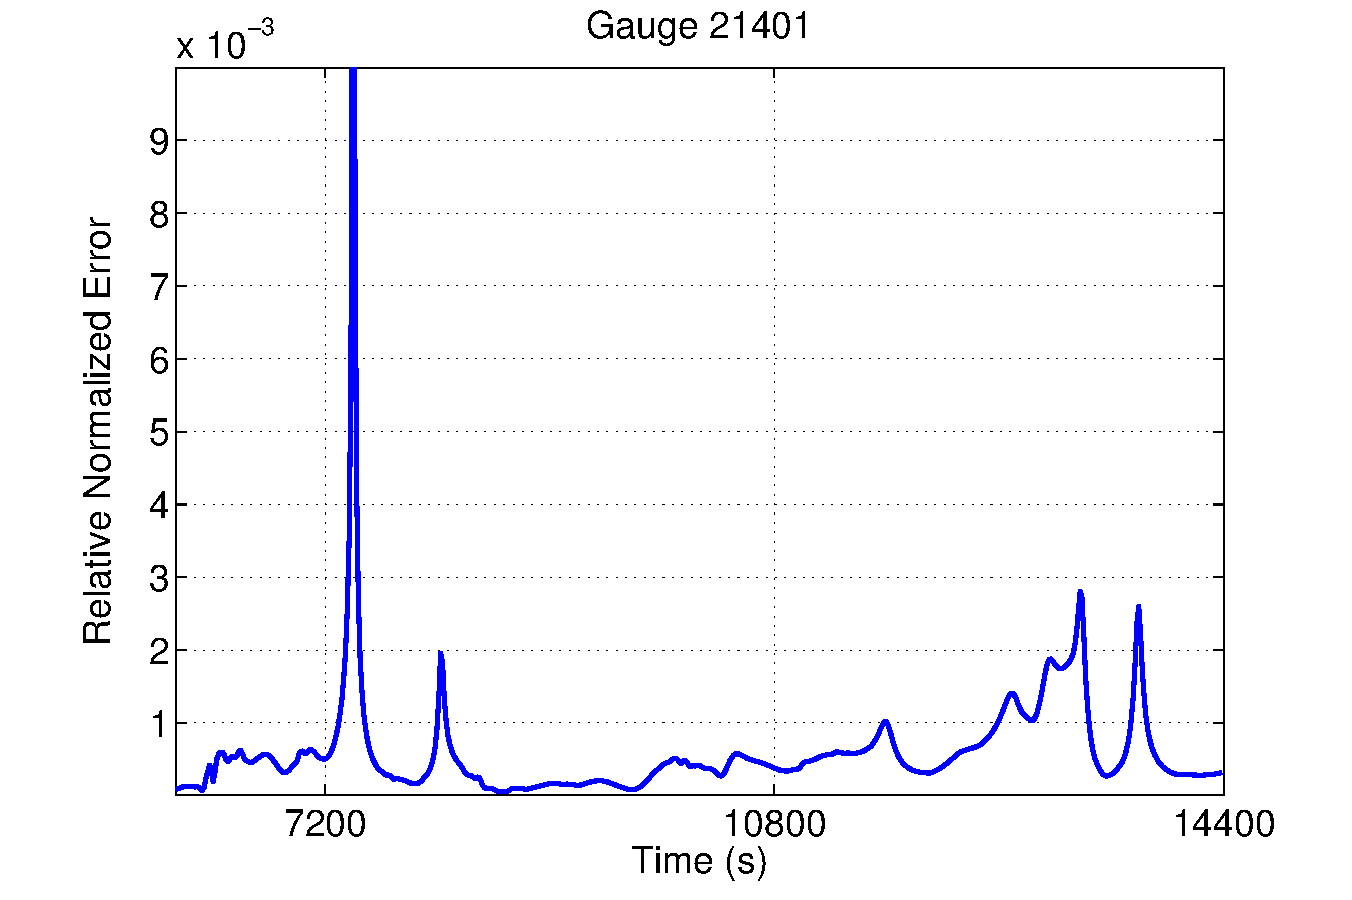
\includegraphics[width=0.5\textwidth]{figures/error_gauge1.pdf} &
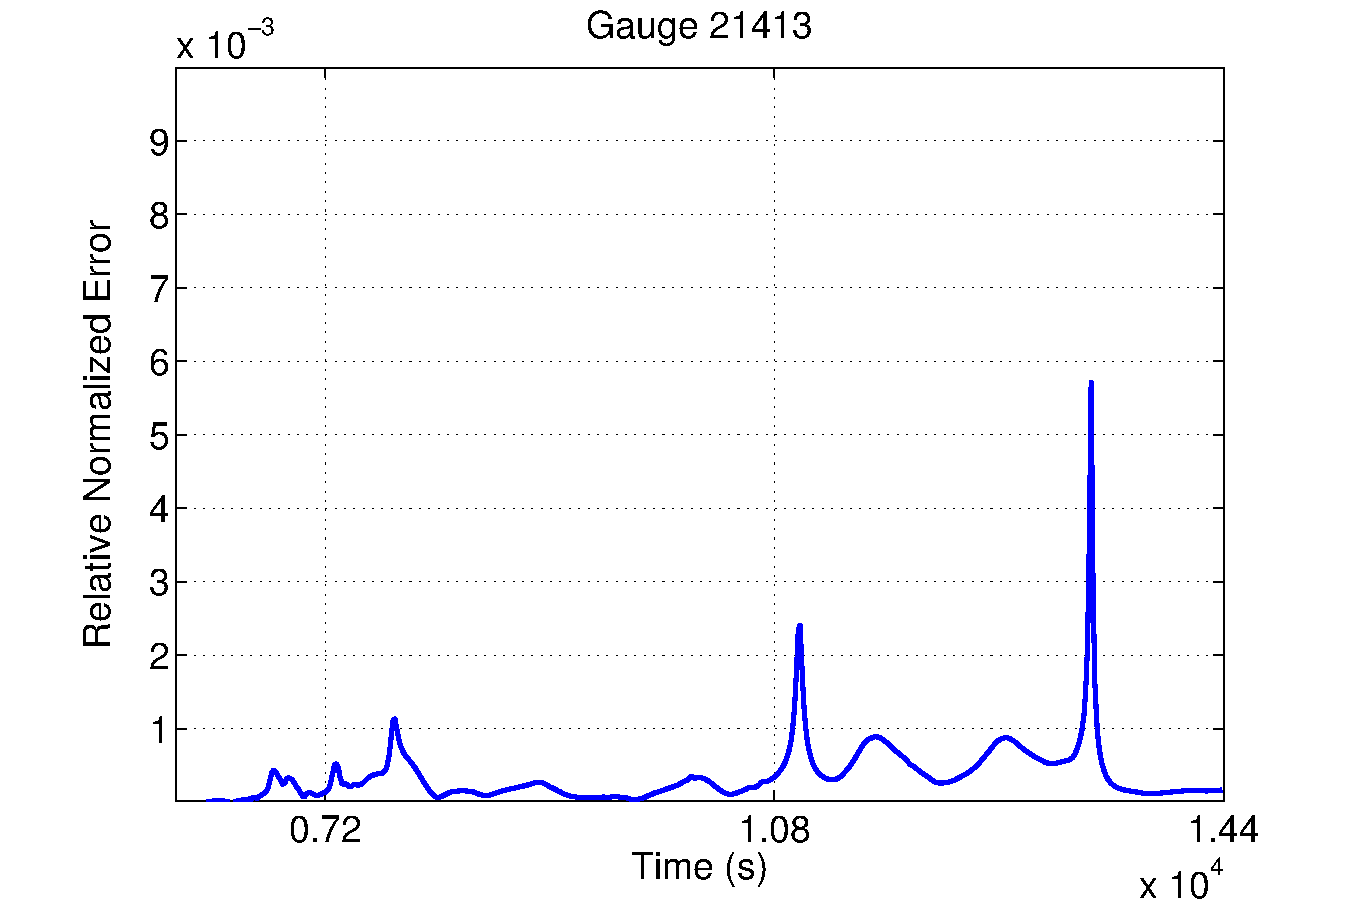
\includegraphics[width=0.5\textwidth]{figures/error_gauge2.pdf} \\
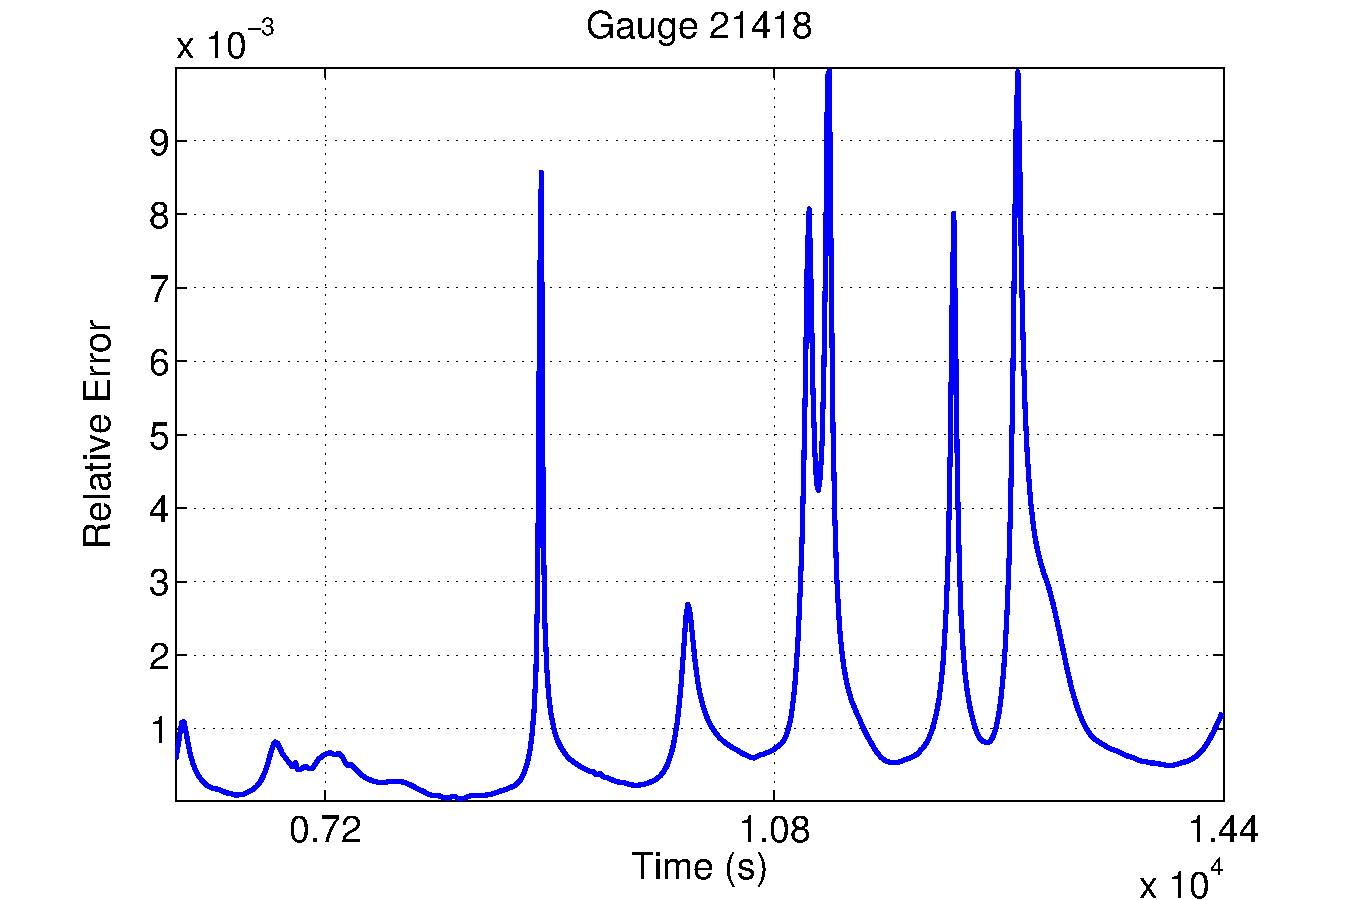
\includegraphics[width=0.5\textwidth]{figures/error_gauge3.pdf} &
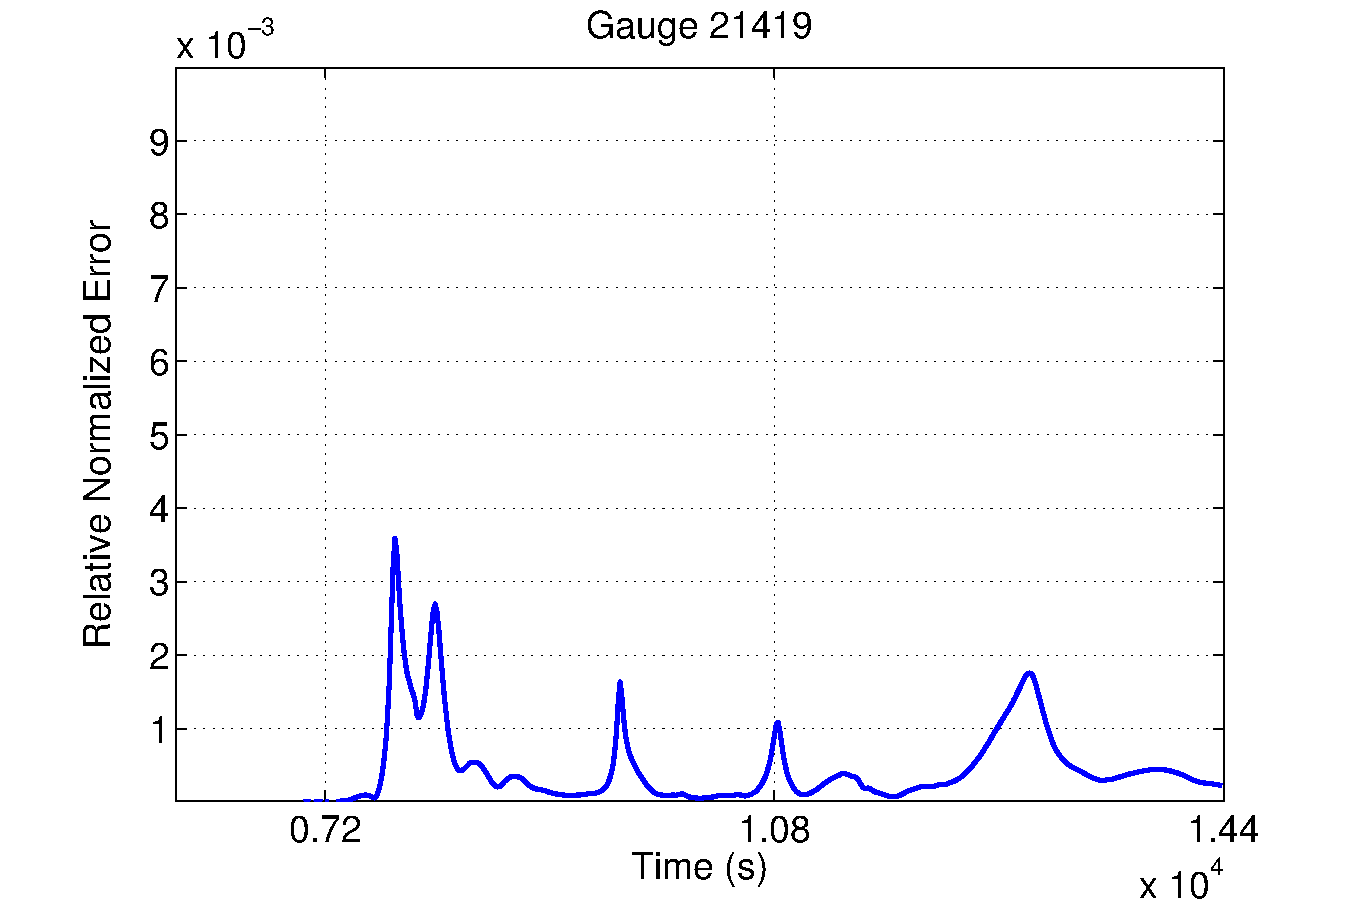
\includegraphics[width=0.5\textwidth]{figures/error_gauge4.pdf} 

\end{tabular}
\caption{125 Geoclaw realizations at different gauge locations.}
\label{fig:error}
\end{figure}

%Contour maps of the relative normalized error for the entire simulation region are 
%shown in Figure~\ref{fig:error2D} for various depths and dates to confirm the error trends of the
%analysis box.  The error is largest after the wind
%intensifies (bottom row) for all depths. For either day, the maximum
%error is located at 50~m which coincides with the depth of the
%original mixed layer measured by the AXBT. The maximum magnitude
%recorded is about 1\% and occurs on Sep~18. The
%elevated error region is located to the right of the storm and
%extends from the surface down to 50~m, after which the impact of the
%input uncertainty decreases substantially.  For the purpose of our
%current study, and given that the majority of AXBT data are at
%depth, the surrogate's errors are considered acceptable and small.

 
A final check consists of verifying whether the probability density
functions (pdfs) of water surface elevation at the different gauge locations
converges with increased order of the PC representation.  Sample
water surface elevation pdfs are shown in Figure~\ref{fig:pdfs2}
and Figure~\ref{fig:pdfs3}

\begin{figure}[h]
\centering

\begin{tabular}{clcl}
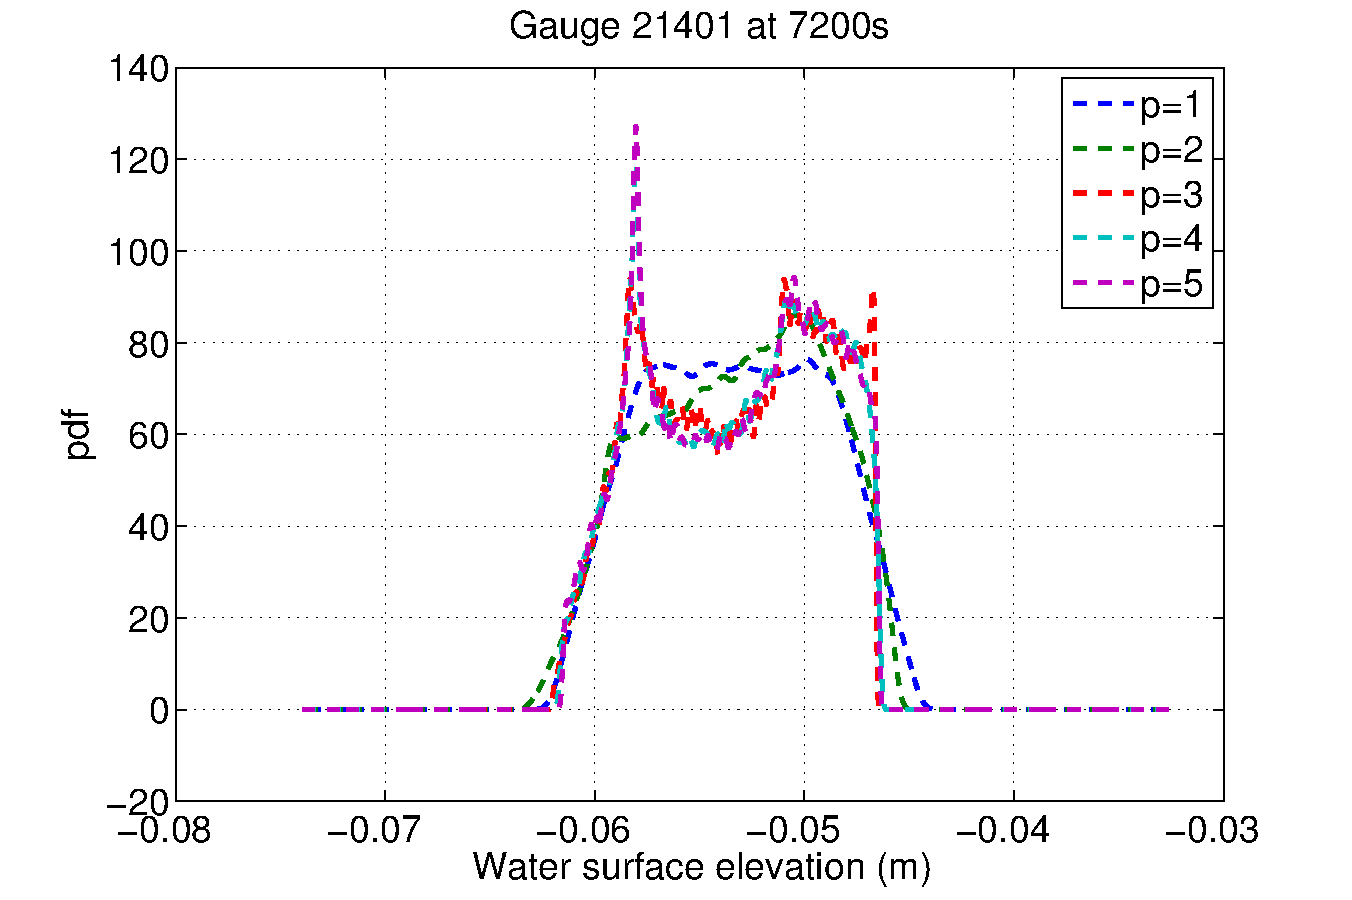
\includegraphics[width=0.5\textwidth]{figures/pdfs1_2.pdf} &
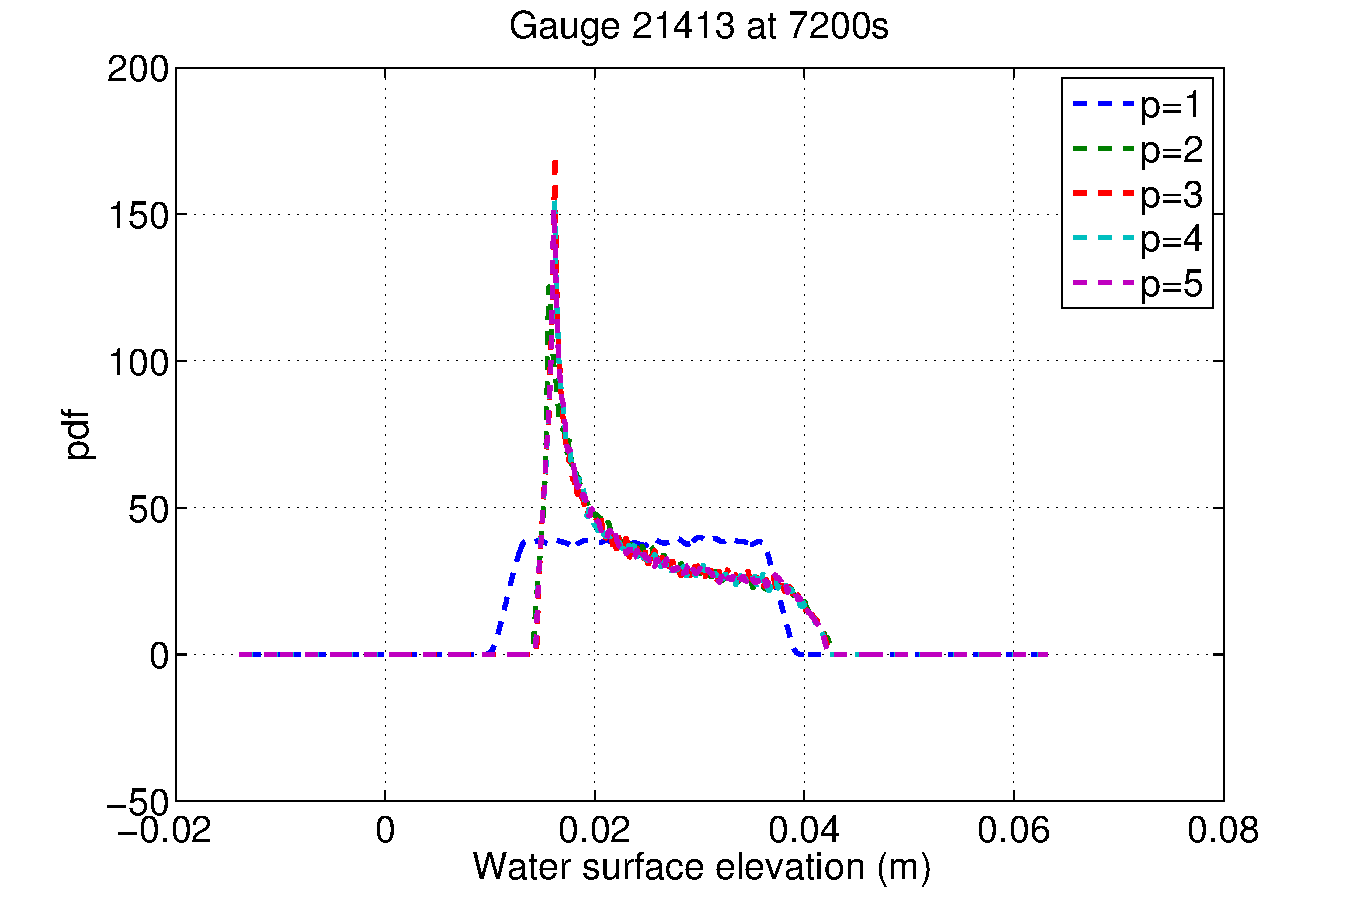
\includegraphics[width=0.5\textwidth]{figures/pdfs2_2.pdf} \\
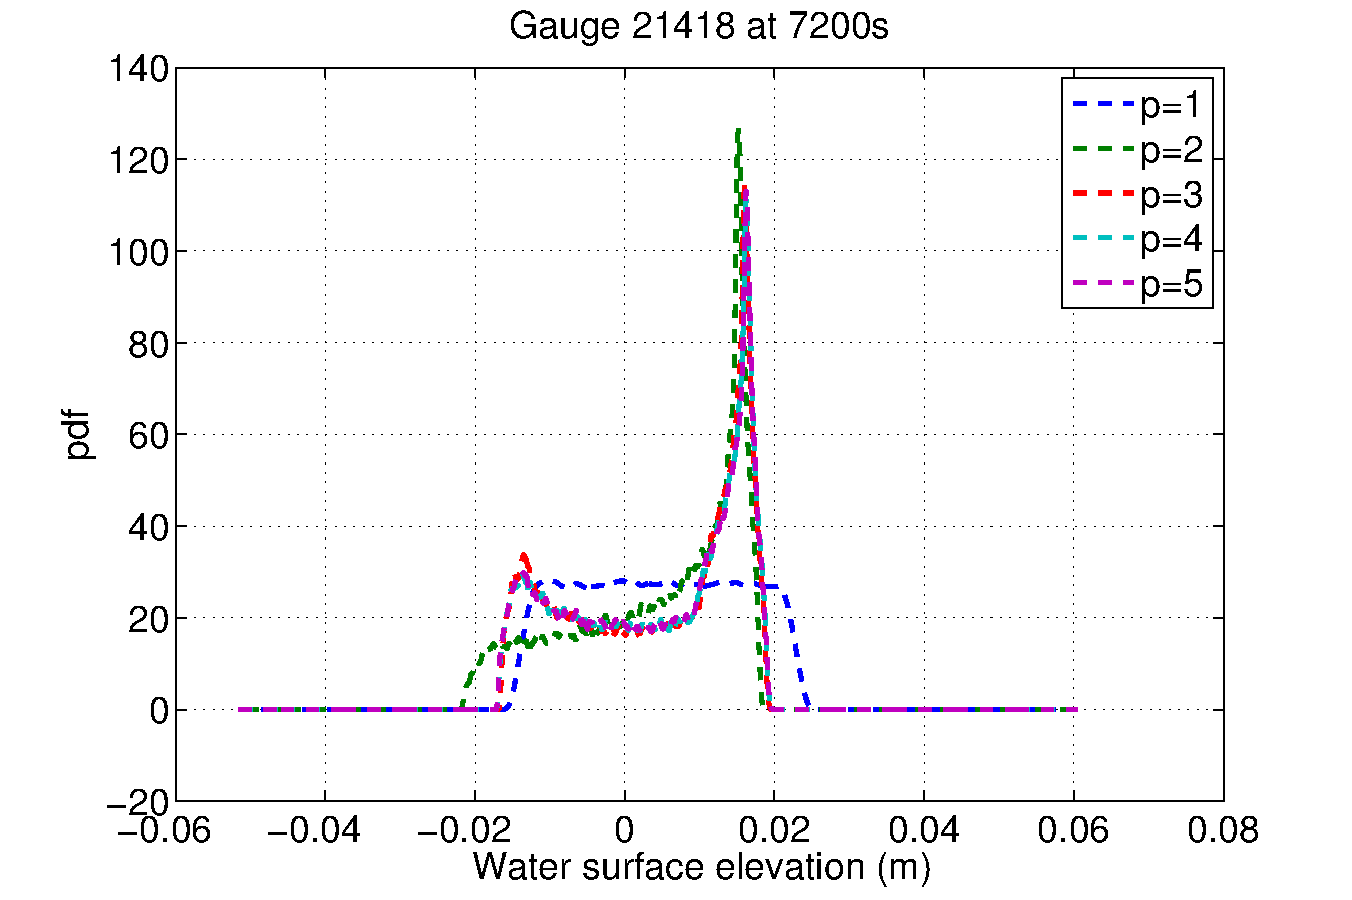
\includegraphics[width=0.5\textwidth]{figures/pdfs3_2.pdf} &
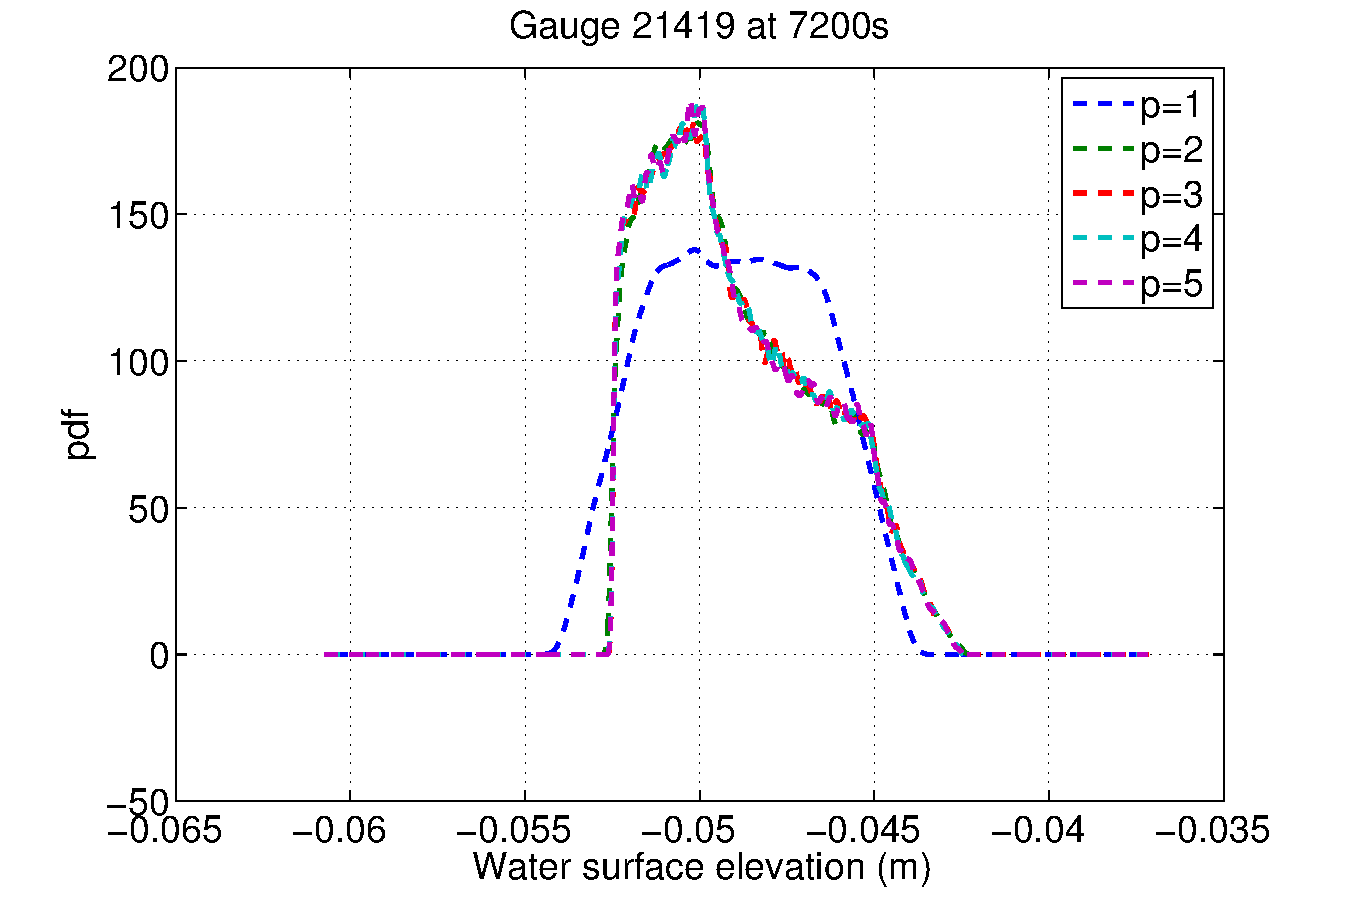
\includegraphics[width=0.5\textwidth]{figures/pdfs4_2.pdf}
\end{tabular}
\caption{pdf of water surface elevation at the different gauge locations at t = 7200 s.}
\label{fig:pdfs2}
\end{figure}
        
\begin{figure}[h]
\centering
\begin{tabular}{clc}
        
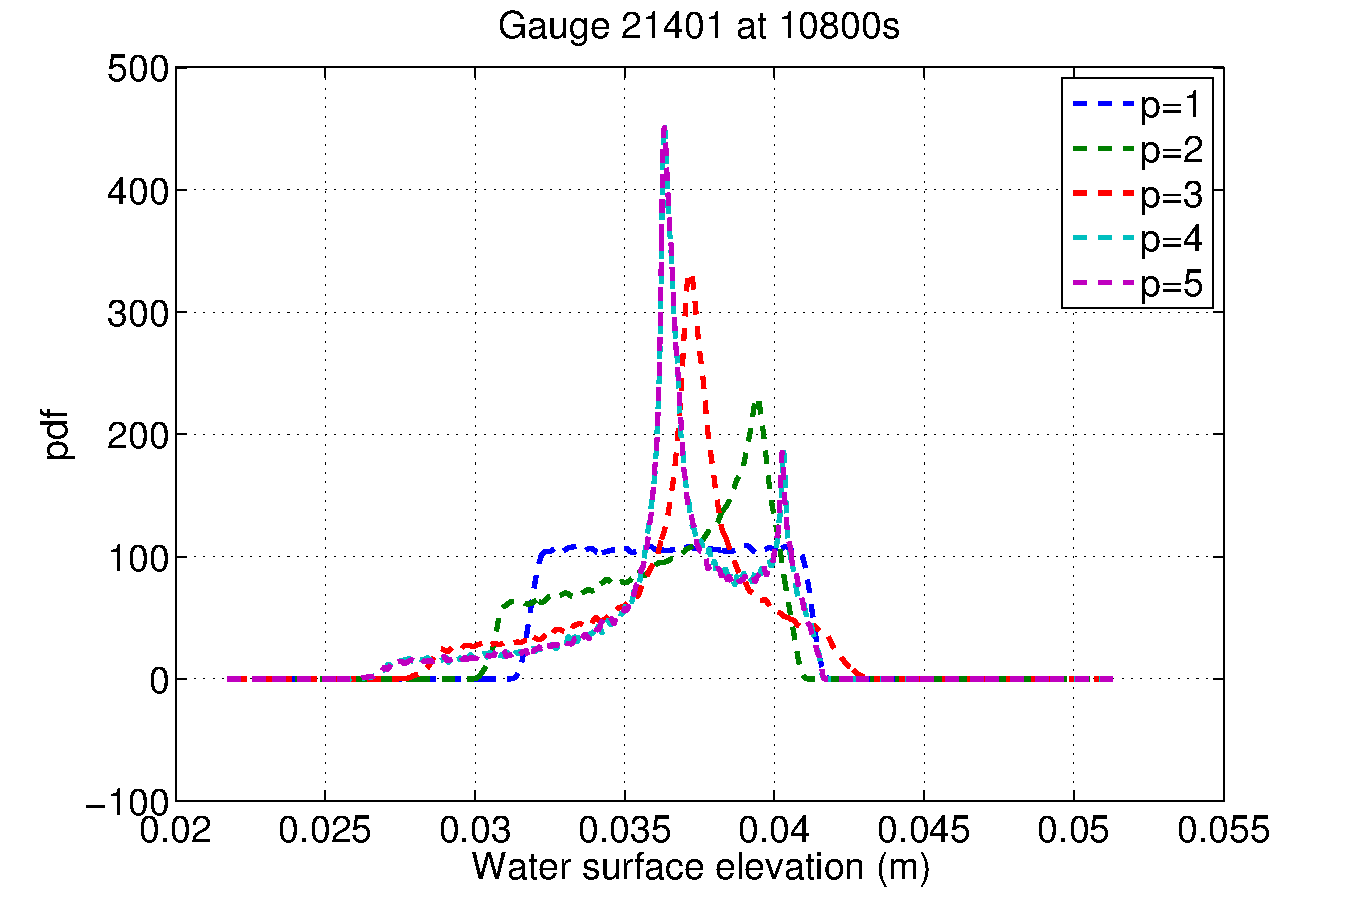
\includegraphics[width=0.5\textwidth]{figures/pdfs1_3.pdf} &
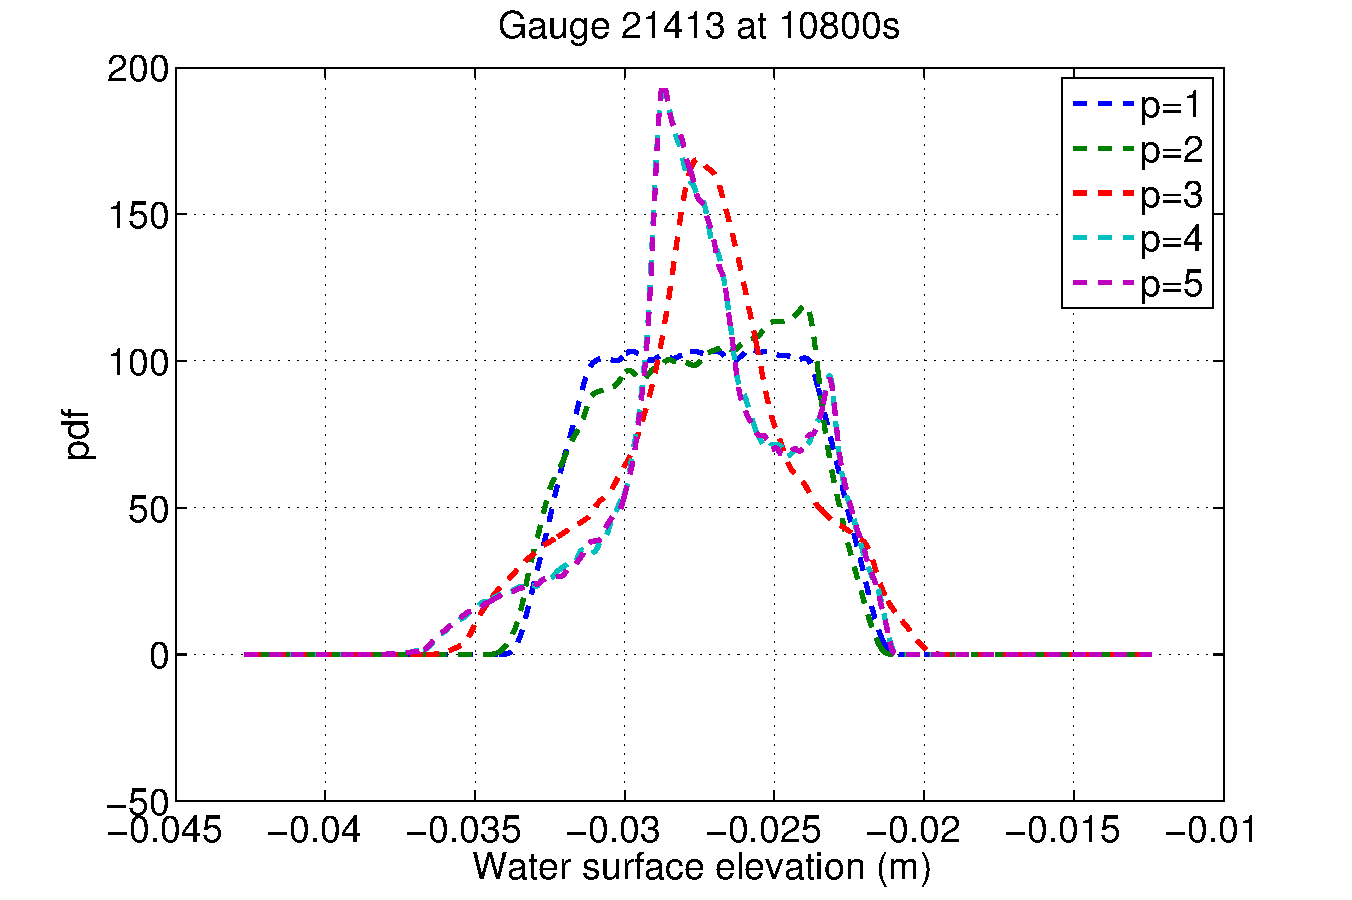
\includegraphics[width=0.5\textwidth]{figures/pdfs2_3.pdf} \\
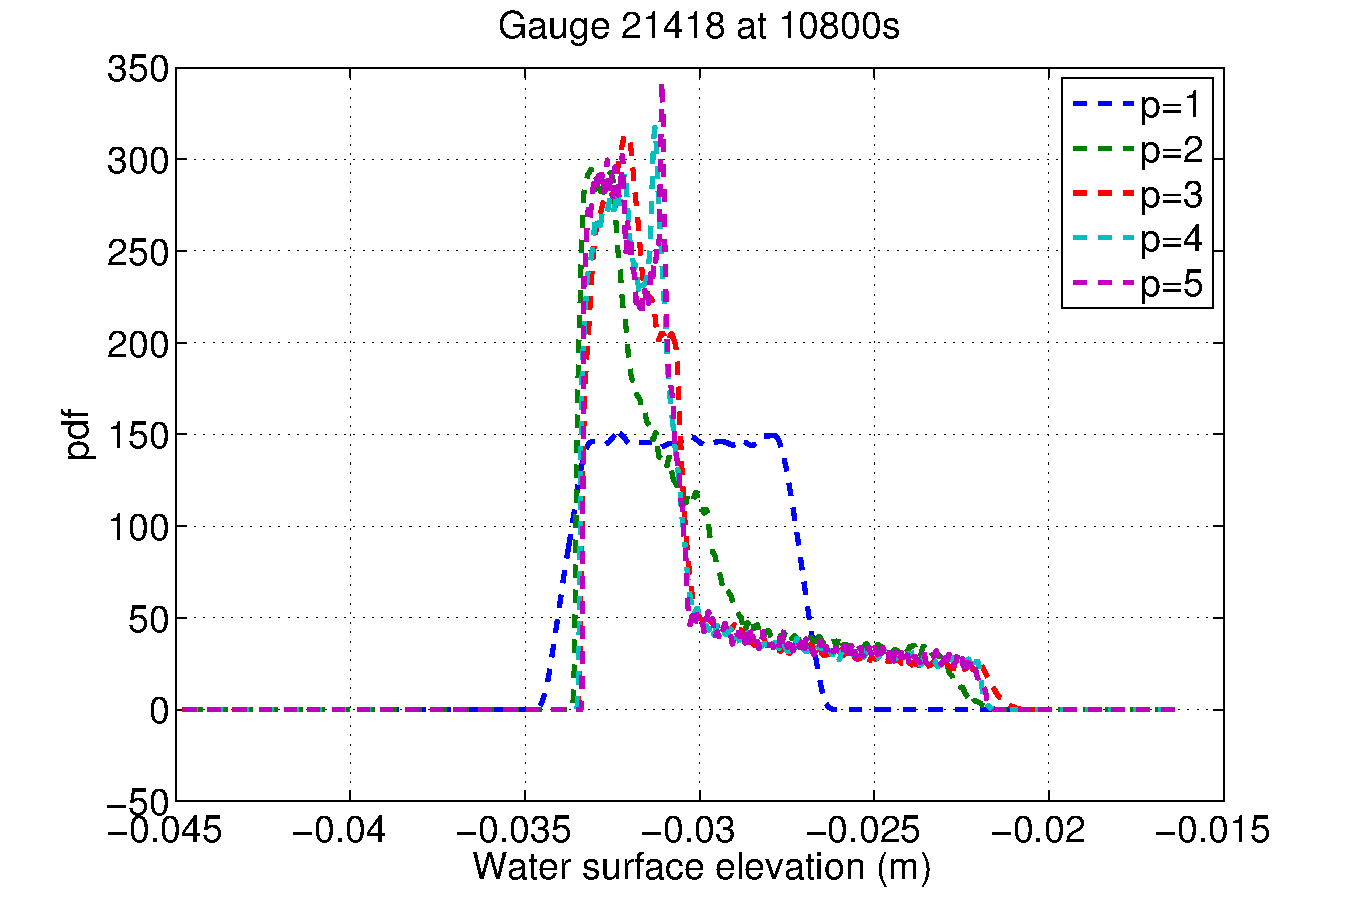
\includegraphics[width=0.5\textwidth]{figures/pdfs3_3.pdf} &
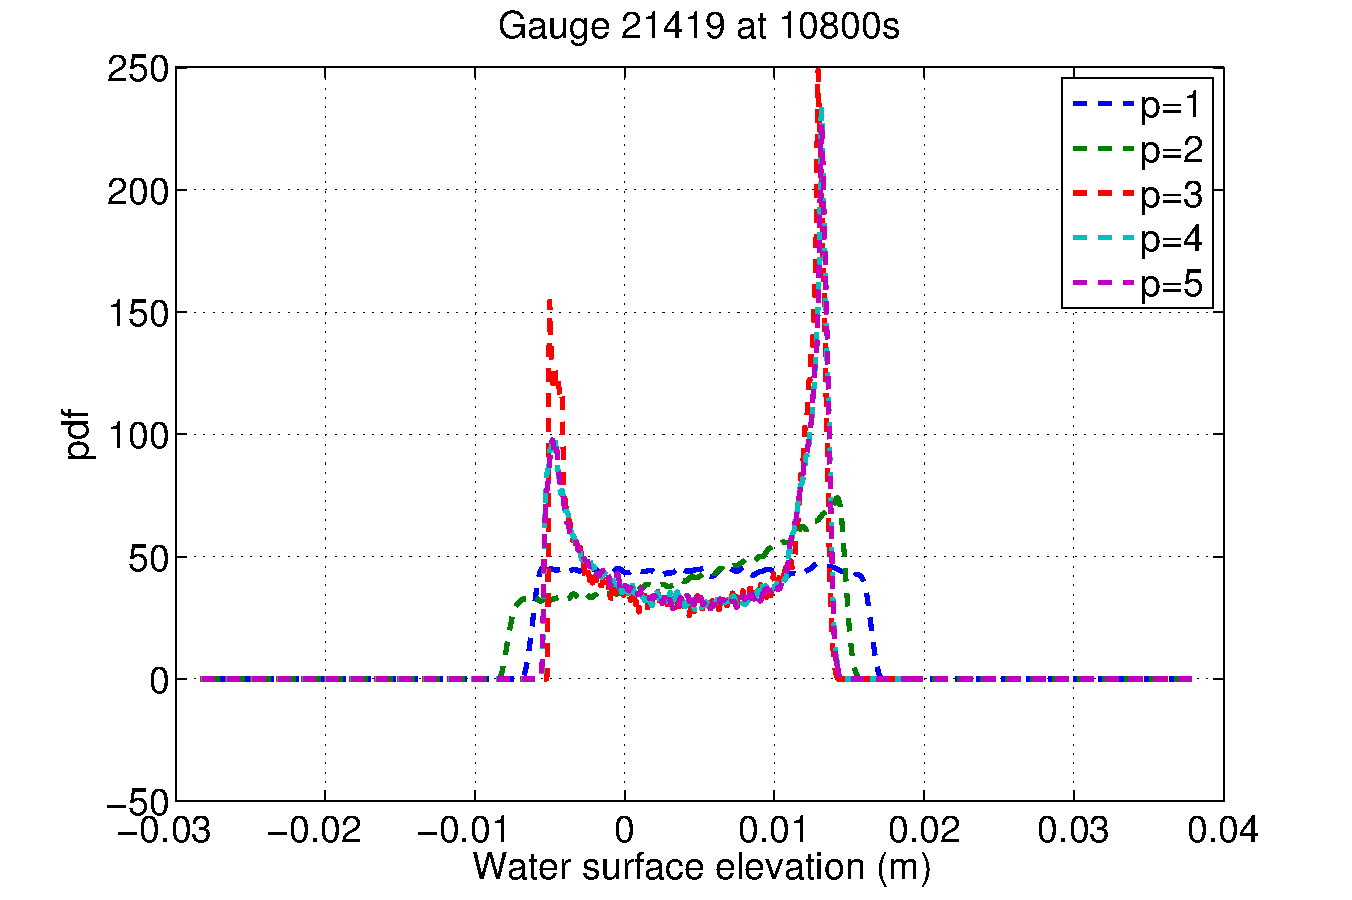
\includegraphics[width=0.5\textwidth]{figures/pdfs4_3.pdf}
\end{tabular}
\caption{pdf of water surface elevation at the different gauge locations at t = 10800 s.}
\label{fig:pdfs3}
\end{figure}
The different curves
correspond to increased order of PC, from 1 to 5; 
The plots indicate that the double peaked distributions are
well-resolved with order  4 but becomes weakly insenstive to further refinement 
as shown with order 5.

The various error metrics presented above 
provide confidence that the PC expansion is a faithful 
model surrogate. 

\clearpage


\subsection{Forward Propagation of Uncertainty}
\label{sec:forward}
The PC expansion created using an ensemble of 125 \geoclaw simulations
is now used as a surrogate to propagate prior input parameter uncertainty 
through the forward model. We here exploit the surrogate 
to study the statistics of the water surface elevation and conduct 
a global sensitivity analysis of the impact of the uncertain input parameters.

\subsubsection{Statistical analysis}
The mean of the QoI and its standard deviation is computed
from the PC coefficients as indicated in Equation~\eqref{eq:mean} and Equation~\eqref{eq:sigma}. 
In Figure~\ref{fig:ave} we plot the evolution of
the calculated PC mean water surface elevation along with two standard deviations
bounds at the four gauges as indicated in each panel.  
Note that we only show the evolution after $t=6000~s$ where the uncertainty is significant,
reflected in a significant standard deviation as seen earlier from the realizations shown 
in Figure~\ref{fig:rlzs}. An interesting observations is that the
standard deviation in water surface elevations vanishes at few times instances
during the tsunami.

These statistics can be used to compare with the 
(DART) buoys observations. Figure~\ref{fig:compare} 
plots the PC mean water surface elevation with the observed 
water surface elevation at the different gauges locations
with error bars indicated at few time instances. 
The plots show a good agreement between the PC simulations and the 
observations at different locations and at different times. 

The same statistical analysis can be performed for the
entire domain in 2D. Figure~\ref{fig:mean2d} (top row) shows
the PC mean water surface elevation for the considered computational
domain at three different times as indicated in the title of each panel.
The standard deviation is also shown in Figure~\ref{fig:mean2d} (bottom row)
at different times. We clearly notice the propagation of the variance
due to the parametric uncertainty with time
and along the tsunami's reflections. 

        
\subsubsection{Sensitivity analysis}
A global sensitivity analysis is next performed to quantity the contribution of each
uncertain parameter to the variance in water surface elevation. To this end, we calculate 
the total sensitivity index using the PC coefficients as shown in Equation~\eqref{eq:T-hard}~\citep{Alexanderian2012,Sudret,Crestaux}. The evolution of the total sensitivity index
of each of the uncertain parameters is shown in Figure~\ref{fig:sens} at the four gauges. 
The Manning's $n$ coefficient at the shore $n_2$ is clearly dominant and contributes
the most to the variance in the water surface elevation compared to the other two 
Manning's $n$ coefficients $n_1$ and $n_3$; this is true for almost the entire simulation time
and at the four gauges. The Manning's $n$ coefficient
in the bottom of ocean $n_{3}$ at gauge number 21419 exhibits small sensitivity index 
during the second hour of simulation and Manning's $n$ coefficient
at the land $n_1$ appears to be an insignificant contributor
to the variance.

In 2D, the sensitivity analysis shows also that $n_2$ is dominant
at the same regions where we observe variance in water surface elevation. This is
indicated from Figure~\ref{fig:sens2d} that shows the total sensitivity index
for $n_1$ (top row) $n_2$ (center row) and $n_3$ (bottom row)
at different times as indicated in each panel.

\subsubsection{Response surface}
In addition to the statistical and sensitivity analysis, the PC surrogate 
can be used to construct a response surface for the uncertain input parameters.
This is achieved by sampling the PC surrogate for different values of the germ $\xxi$ within the prior
range. Since $n_3$ shows insignificant contribution to the 
uncertainty in the model output, we find the impact of $n_2$ and $n_3$ for 
fixed value of $n_1=0.1025$ as illustrated in Figure~\ref{fig:response2}
and Figure~\ref{fig:response3} for different times as indicated. The most striking features are the relatively flat
horizontal contours in the $n_3$ direction suggesting that water surface elevation depends
only mildly on $n_3$ even during peak tsunami events. This is true for gauges 21401, 21413 and 21418. However,
at gauge 21419, its the opposite case where the horizontal contours are in the $n_2 $ direction
and there water surface elevation depends mildly on $n_2$.

\subsection{Inverse Problem} 
\label{sec:inverse}

Before attempting solving the inverse problem,
we need to make sure that the observed data are
comparable to the simulated one. To this end, Figure~\ref{fig:compare}
compares PC mean water surface elevation profiles (with error bars)
with their counterparts from the observed gauge locations.
The plots show a good agreement between the simulations and the 
observations at different locations and at different times. 
The same comparison can be recast as a scatter plot shown in 
Figure~\ref{fig:scatter}. The difference between the observations
and simulations is attributed to the uncertainty in the 
Manning's N coefficient and to the measurement errors to be quantified
in this section.

The surrogate model is exploited in the Bayesian inference of the Manning's 
roughness coefficient.  To this end, an adaptive MCMC method is used to sample 
the posterior distributions \citep{Gareth2009,Haario2001} and consequently 
update the Manning's roughness coefficient distributions in light of the 
observed data. This sampling, demanding tens of thousands of forward simulations, 
would have been prohibitively expensive in the
absence of the surrogate, as the generation of each sample would have required an
independent \geoclaw realization. The surrogate provides a computationally
efficient alternative, and requires only evaluating the PCE for different values 
of the seed $\xxi$. The setup of the Bayesian inference problem,
MCMC chains for the input drag parameters and the corresponding posterior distributions are 
presented and discussed in this section. 


The observed data collected at different locations 
in the likelihood function (Equation~\eqref{eq:likelihood}) to update the input parameters.
MCMCs of $50,000$ iterations are obtained for the Manning roughness coefficients: 
$N_1$,$N_2$ and $N_3$ as well as for the variance $\sigma^2$. Figure \ref{fig:mcmc} 
shows the sample chains for
the input parameters for different iterates of the MCMC algorithms. 
The different panels
shows well-mixed chains for all parameters.
However, all chains span the entire range
of the prior, and so it appears that the observations are not informative 
concerning this uncertain input.  $N_{2}$ chain appears to be concentrated in the lower end of the
parameter range, with values between 0.005 and 0.1.
The chain for the variance is also shown in 
Figure~\ref{fig:mcmc} and appears to be well mixed.





The computed MCMC chains can be readily used to determine the posterior 
distribution; kernel density estimation (KDE) is used for this purpose
~\citep{Parzen1962,Silverman1986}(The first 5000 iterates, associated 
with the burn-in period, are discarded). The resulting posterior pdfs 
of the three Manning's roughness coefficients $N_1,N_2,N_3$ are shown 
in Figure~\ref{fig:pdfs}.  As expected from the chains shown in Figure
~\ref{fig:mcmc}, the posterior pdf of $N_2$, exhibits well-defined peak, 
with a Maximum A Posteriori (MAP) estimate of around 0.011; an extended tail 
towards the higher Manning's roughness coefficient values is also observed.
In contrast, the posterior pdfs of $N_1$ appear to be fairly flat, 
and similar to the uniform prior. This is an indication that 
the observed data were not useful to refine our prior knowledge for $N_1$.
While for $N_3$, we observed a posterior that has a well defined peak
of 0.185 but no clear pdf shape.
The posterior distribution of the variance is also shown in Figure~\ref{fig:mcmc}. 
Taking the square root of the MAP values yields the water surface elevation standard 
deviation, and the latter is a reflection of the mismatch between the model and 
observed data estimated to be 0.145~$m$.


   %MAPS 0.021308543478839   0.011083123405057   0.185744276109897   0.021045124706835





%!TEX root = paper.tex
\section{Discussion and Conclusions}
\label{sec:conc}

The present study aimed at estimating Manning's $n$ friction coefficient  which
plays an important role in the accurate prediction of water surface elevation in
tsunami modeling. We proposed a three-parameter representation of Manning's $n$
friction coefficient that was characterized using iso-baths  to define three
distinct regions, on-shore, near-shore, and deep-water, in the domain and
represented each region with a single Manning's $n$ coefficient.  The estimation
relied on a Bayesian inference approach that sharpens the initial estimates of
the three uncertain parameters using real observations.

In our test case, the \tohoku tsunami, we used four DART buoy gauges that
provide  surface elevation information.  To accelerate the Bayesian inference,
we relied on the polynomial  chaos expansions to produce a faithful and
efficient surrogate of the forward model \geoclaw.  This PC surrogate model was
then used to quantify the uncertainties in the predicted water surface
elevations due to the uncertainties in the Manning's $n$ coefficient.  This
included the mean and standard deviation of water surface elevations which were
also compared to the measured buoy data.  A global sensitivity analysis was also
performed in order to quantify the contribution of each uncertain parameter to
the variance in surface elevation.  It was found that the Manning's $n$
coefficient in the near-shore region $n_2$ contributed the most to the variance
in the surface elevations compared to the other two Manning's $n$ coefficients
in the on-shore and deep-water regions.  This is expected as the deep-water
friction has little effect on the overall column.  On the other hand, the
sensitivity of the analysis to the on-shore value being less than that in the
deep-water was unexpected. We suspect that this is primarily due to the use of the
DART buoy gauges, being far enough from land regions to have a significant impact. 
This might not be the case if data from inundation zones (that
were not available to us) were used. 

Using Bayesian inference, MAP estimates were found for the three region's $n$
parameters using MCMC.  These values were (excluding $n_1$ where no meaningful
MAP value was found), $n_2=0.011$ and $n_3=0.180$.  The values and their
corresponding marginalized PDFs tell perhaps the most
complete story in this analysis.  As mentioned earlier, $n_2$ is the most
sensitive and has the most clear MAP value.  Although the value was lower than
expected, the tail includes the most commonly used values (0.022-0.025).  The
deep-water value $n_3$ has a peak that is much higher than expected but a tail
that does not taper off particularly quickly.  This is not altogether unexpected
due to the low sensitivity of the QoI to this region's friction.  The
on-shore value $n_1$ shows again how insensitive the used simulations and
observations were to on-shore values in our particular setting.  
In conclusion, it is clear that the use of only the DART buoy observations and the 
bathymetry resolution used here is not sufficiently informative to invert for the 
Manning's $n$ values with any strong confidence, especially outside of the near-shore region.

Finally, it should be noted that the friction source term is only one of a
number of other sources of uncertainty.  In particular, the rupture model and
bathymetry might often have an important influence on the tsunami.  
In the future, this type of analysis would be more illustrative if
propagation of uncertainties in both the bathymetry and source models were
included in each Manning's $n$ estimate.  The
present study focused on formulating and estimating a low-dimensional
representation of the Manning's $n$ coefficient using UQ techniques, namely
Bayesian inference and PC expansions.  A high-dimensional representation of the
Manning's $n$ coefficient would require a large number of forward runs and this remains
computationally expensive.  We will work on alternative methods to reduce the
dimensionality of the problem and this will be the objective of a future study.


\clearpage

%!TEX root = paper.tex
\begin{figure}[ht]      
\centering
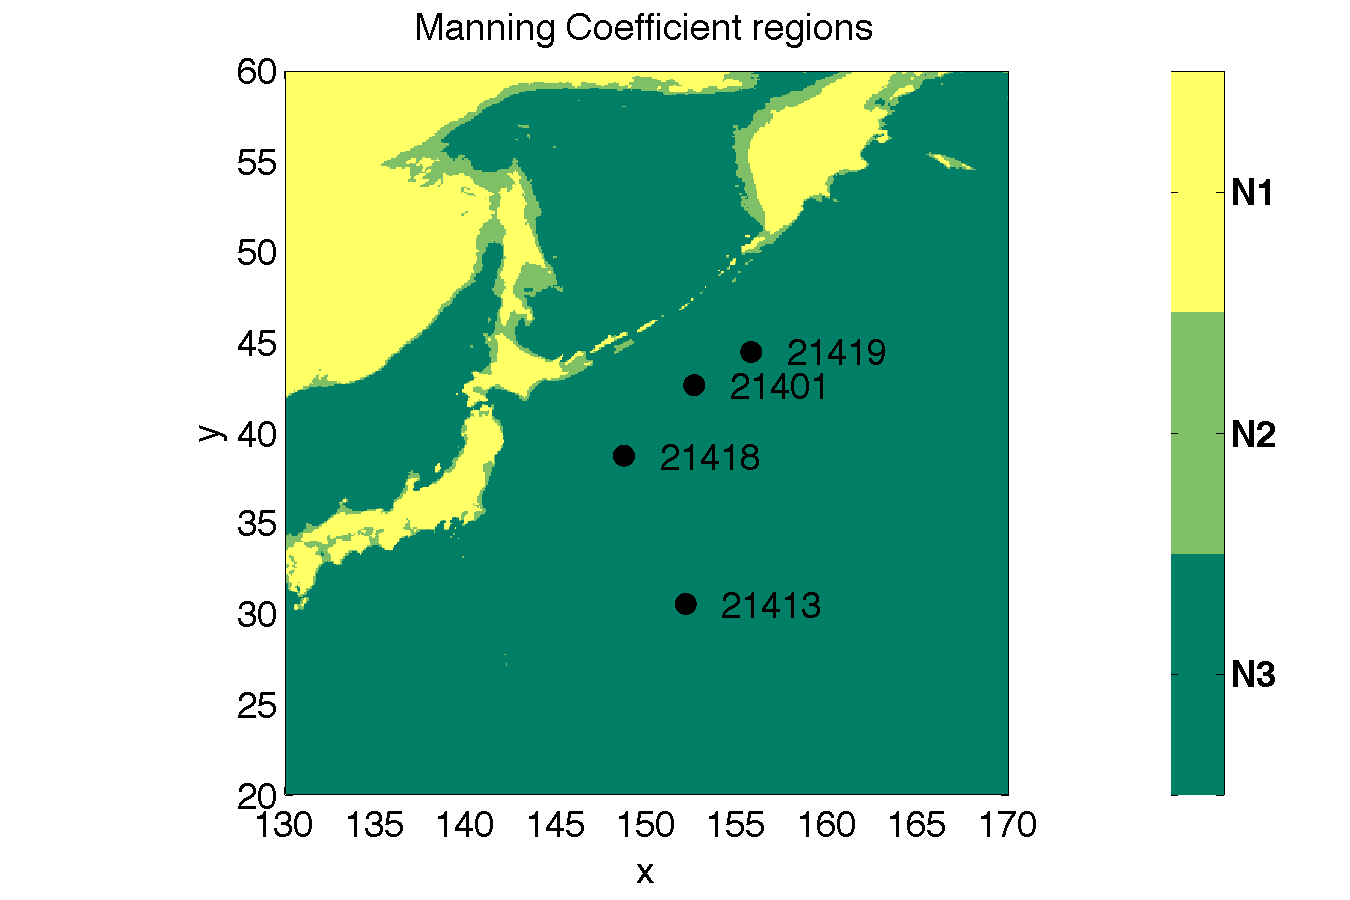
\includegraphics[width=0.6\textwidth]{./figures/coef.pdf}
\caption{Manning's $n$ coefficients at three regions: $n_1$ on-shore, $n_2$ near shore, $n_3$ deep-water.}
\label{fig:ceofs}
\end{figure}  
%%%%%%%%%%%%%%%%%%%%%%%%%%%%%%%%%%%%%%%%%%%%%%%%%%%%%%%%%%%%%%%%

\begin{figure}[ht]
\centering
\begin{subfigure}[c]{0.45\textwidth}
    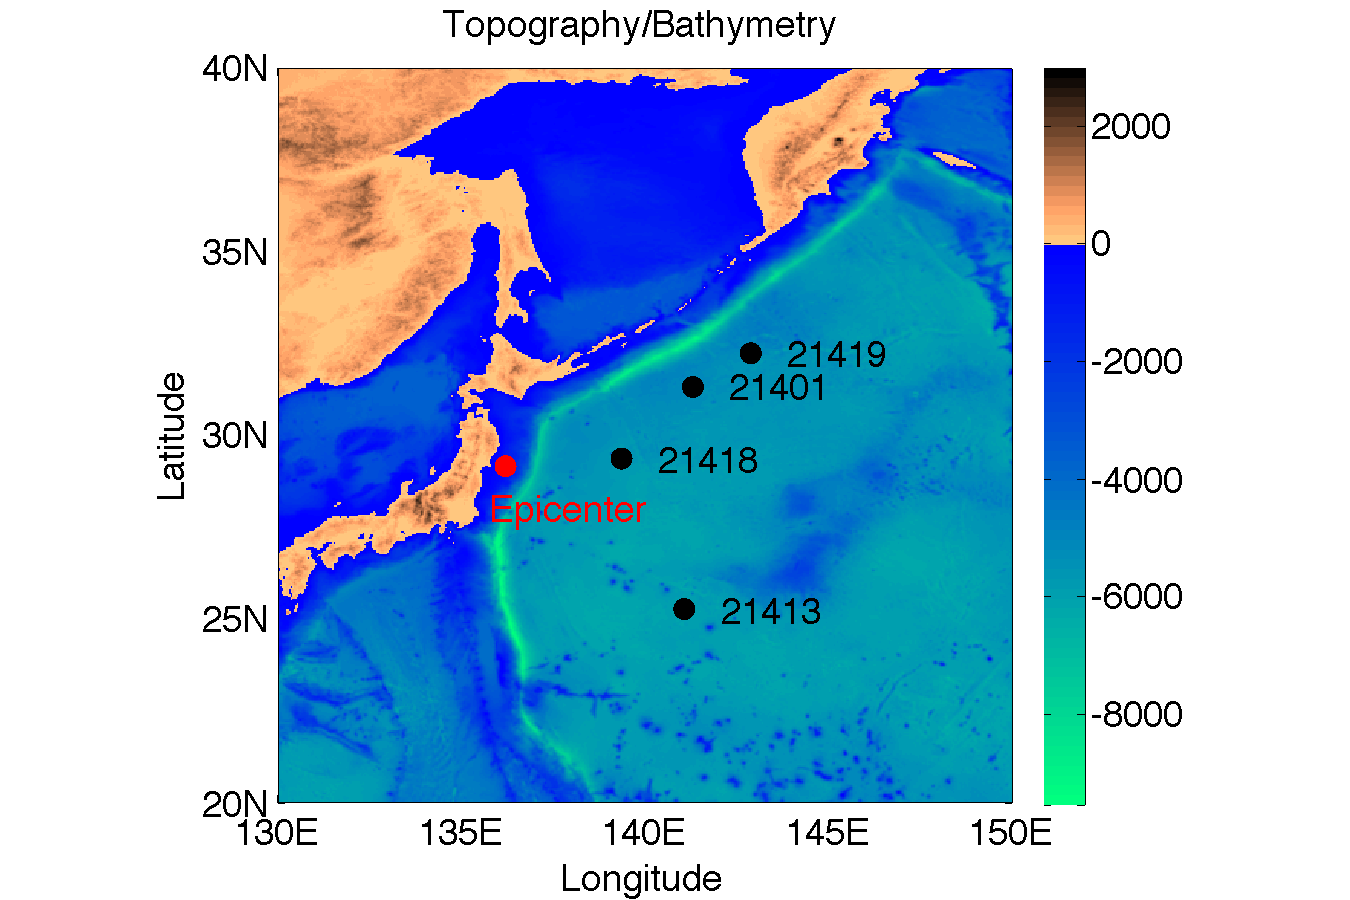
\includegraphics[width=\textwidth]{./figures/topo.pdf}
    \caption{} \label{fig:setup_buoy_locations}
\end{subfigure}
\begin{subfigure}[c]{0.45\textwidth}
    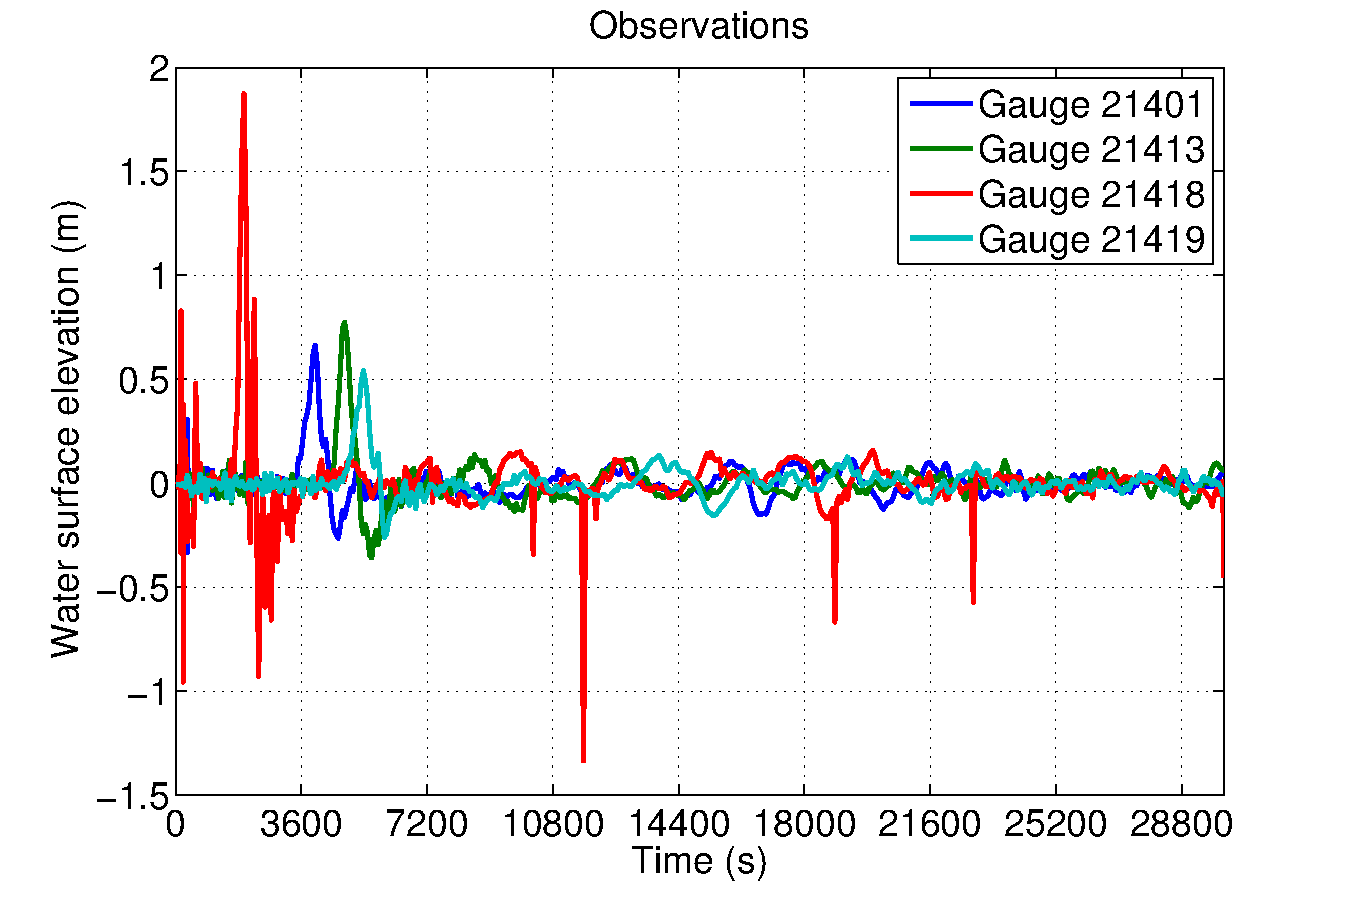
\includegraphics[width=\textwidth]{./figures/obs.pdf} 
    \caption{} \label{fig:setup_buoy_data}
\end{subfigure}
\caption{(a) The topography, bathymetry and gauge locations used in the simulation. (b) Observed de-tided water surface height at all the DART buoys used.}
\label{fig:setup}
\end{figure}

%%%%%%%%%%%%%%%%%%%%%%%%%%%%%%%%%%%%%%%%%%%%%%%%%%%%%%%%%%%%%%%%
\begin{figure}[ht]
\centering
\begin{tabular}{clc}        
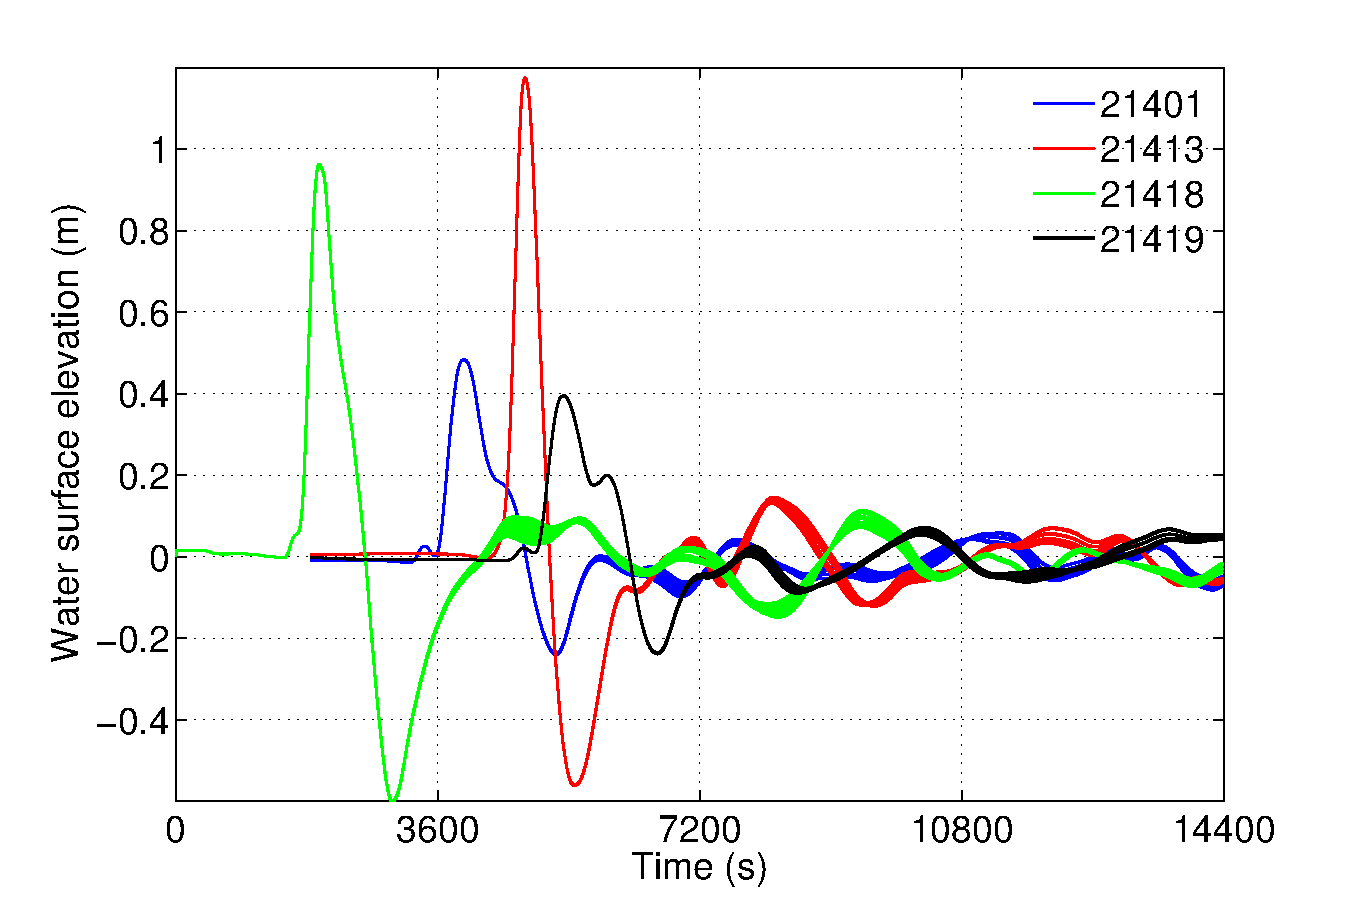
\includegraphics[width=0.6\textwidth]{./figures/rlzs_gauges.pdf} 
\end{tabular}
\caption{125 \geoclaw realizations at different gauge locations.}
\label{fig:rlzs}
\end{figure}
%%%%%%%%%%%%%%%%%%%%%%%%%%%%%%%%%%%%%%%%%%%%%%%%%%%%%%%%%%%%%%%%

\begin{figure}[ht]
\centering
\begin{tabular}{clc}        
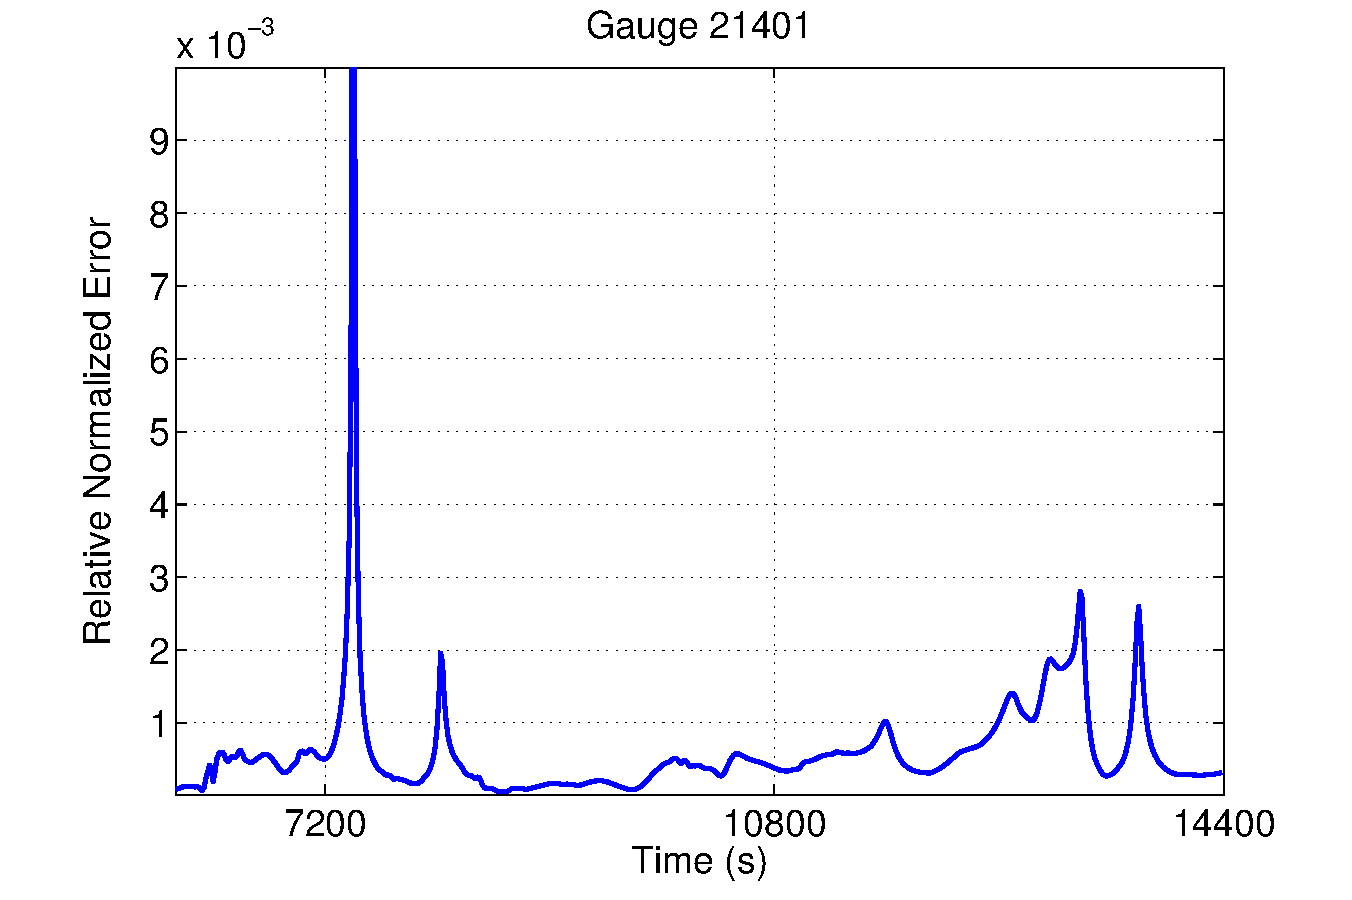
\includegraphics[width=0.5\textwidth]{./figures/error_gauge1.pdf} &
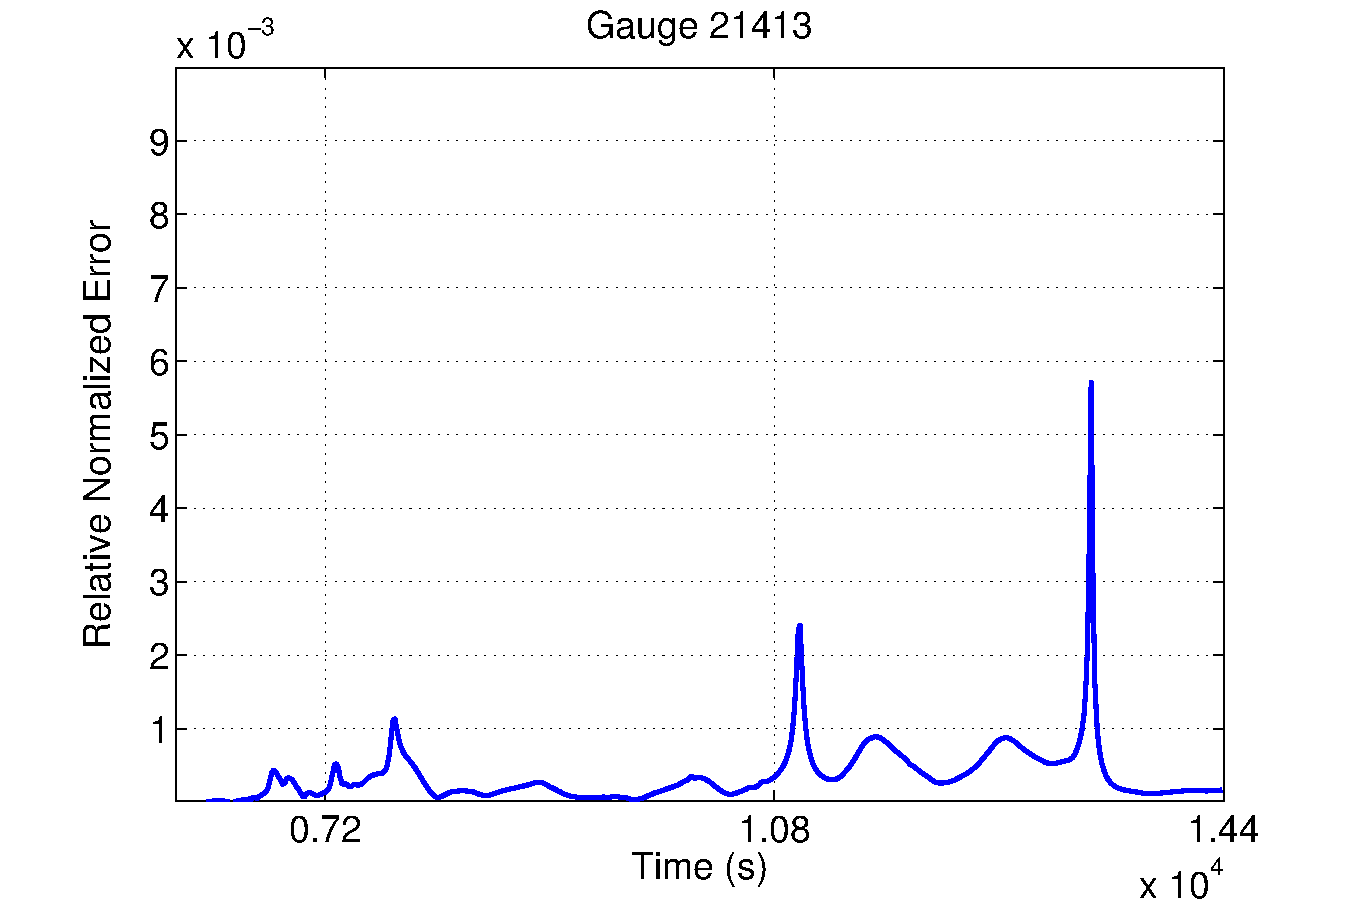
\includegraphics[width=0.5\textwidth]{./figures/error_gauge2.pdf} \\
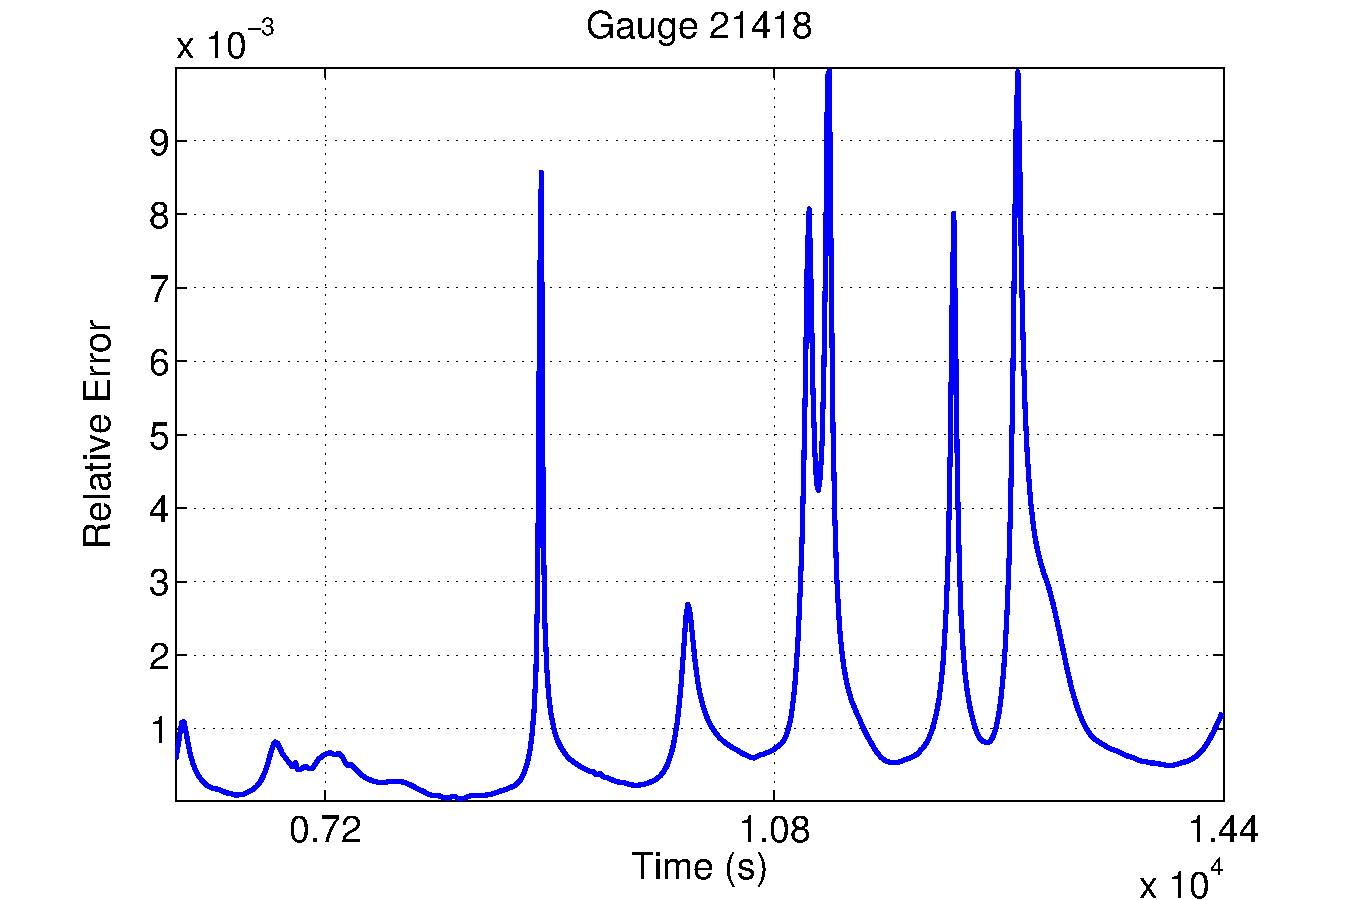
\includegraphics[width=0.5\textwidth]{./figures/error_gauge3.pdf} &
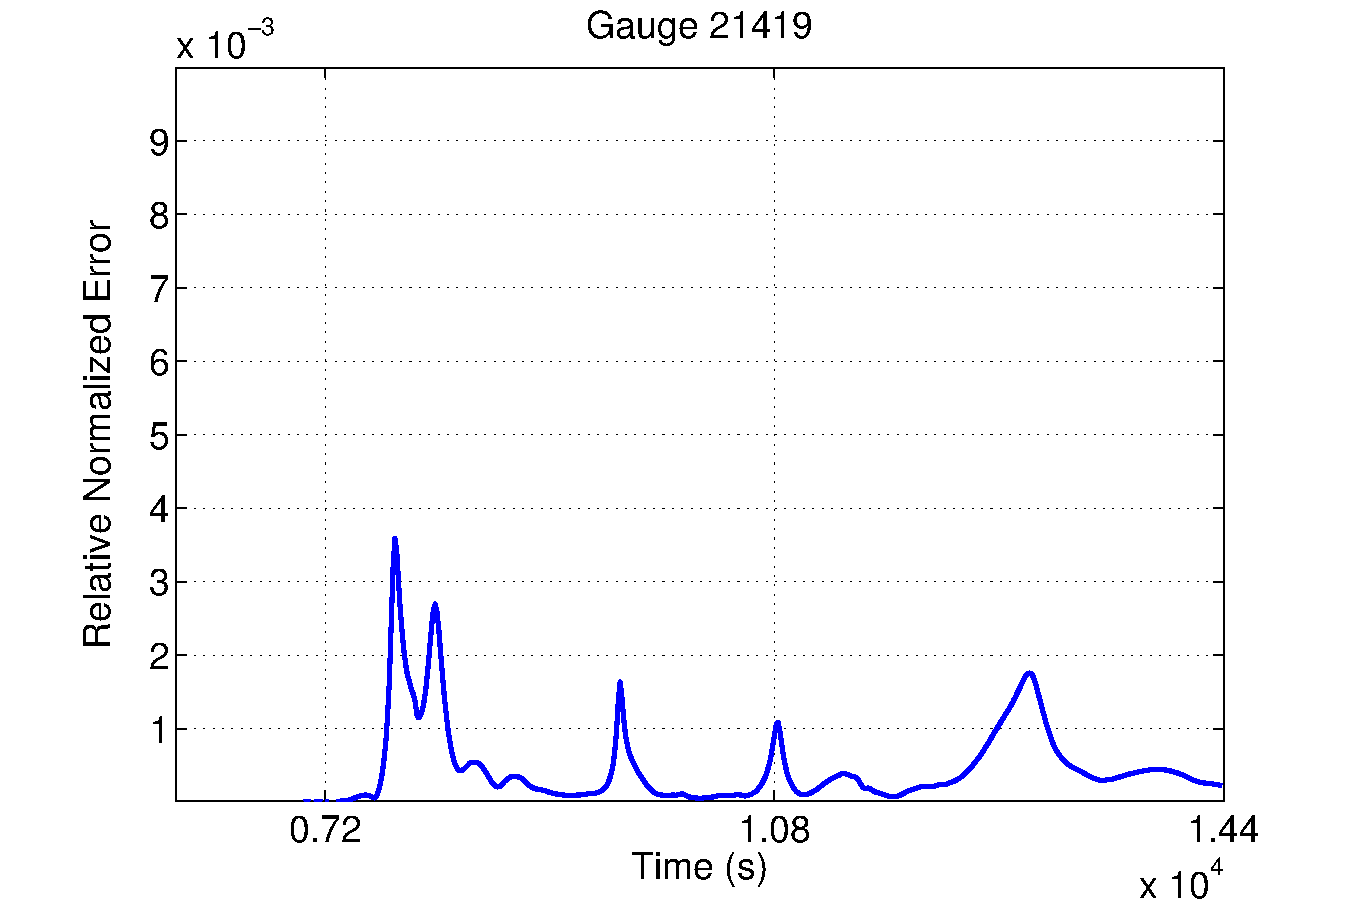
\includegraphics[width=0.5\textwidth]{./figures/error_gauge4.pdf} 

\end{tabular}
\caption{Relative normalized error between realizations and 
the corresponding PC surrogates at different gauge locations
calculated using Equation~(\ref{eq:error}).}
\label{fig:error}
\end{figure}   
%%%%%%%%%%%%%%%%%%%%%%%%%%%%%%%%%%%%%%%%%%%%%%%%%%%%%%%%%%%%%%%%
\begin{figure}[ht]
\centering

\begin{tabular}{clcl}
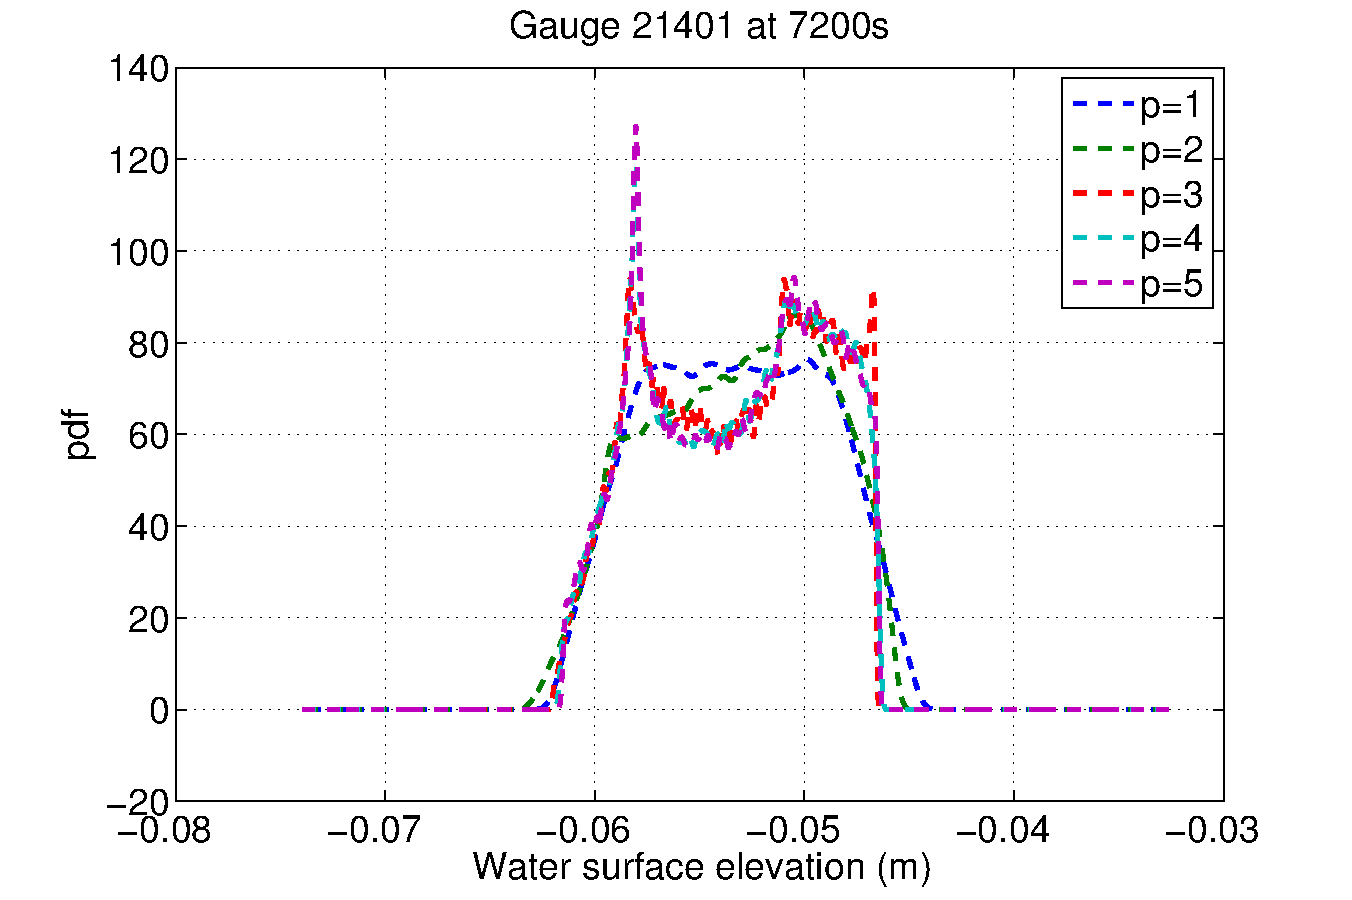
\includegraphics[width=0.5\textwidth]{./figures/pdfs1_2.pdf} &
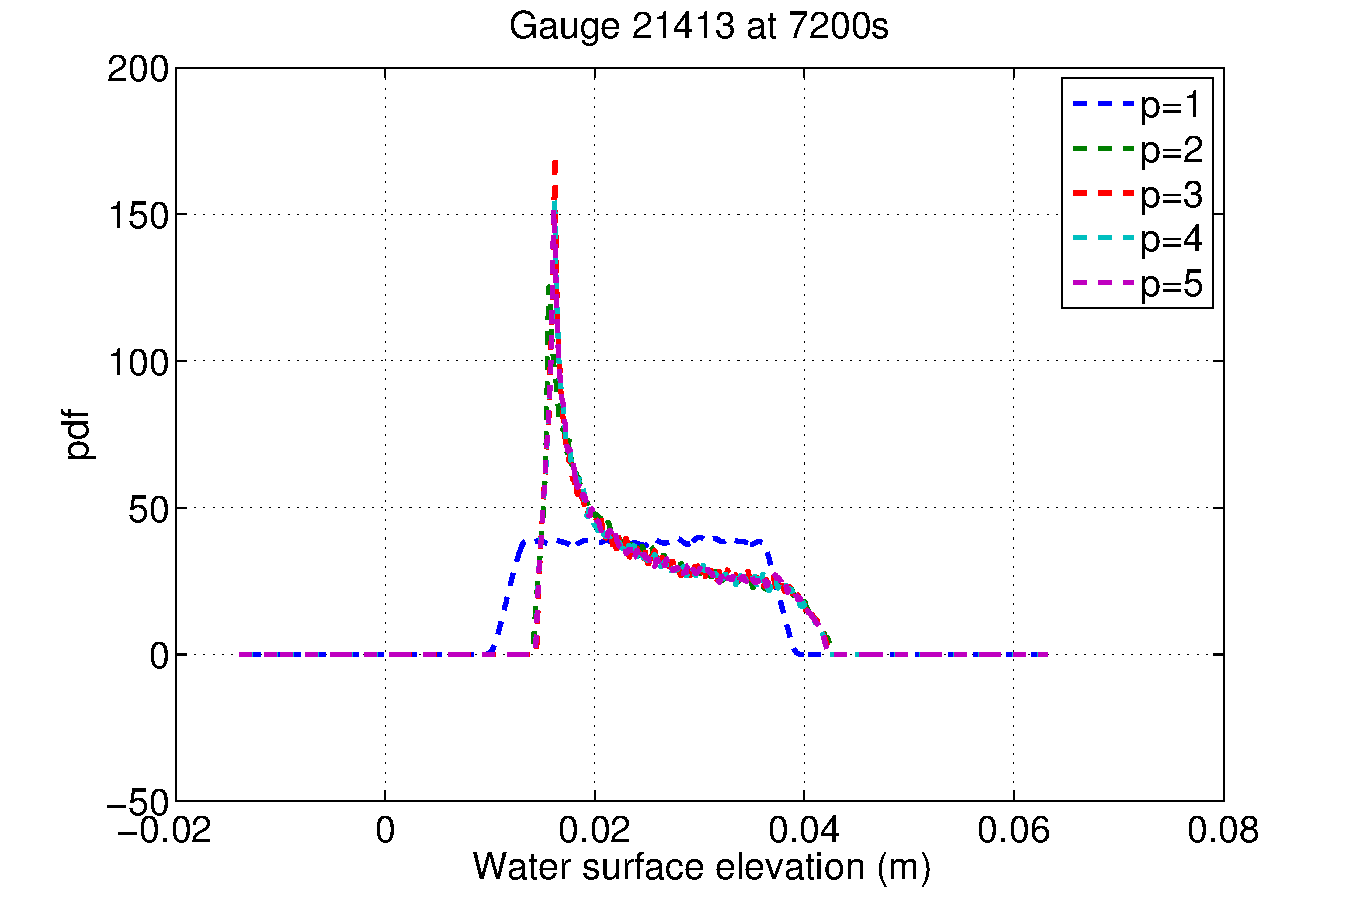
\includegraphics[width=0.5\textwidth]{./figures/pdfs2_2.pdf} \\
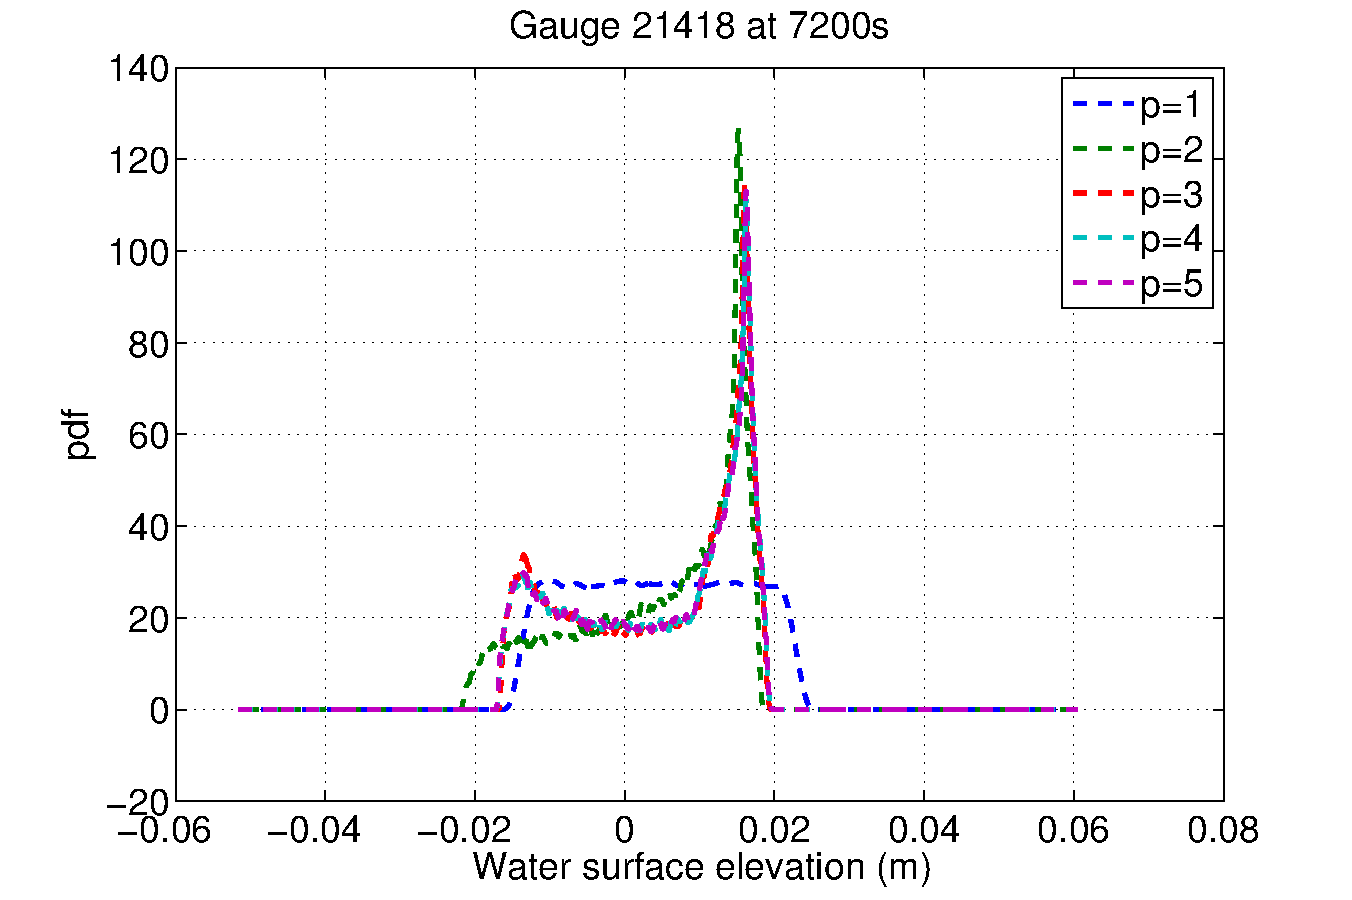
\includegraphics[width=0.5\textwidth]{./figures/pdfs3_2.pdf} &
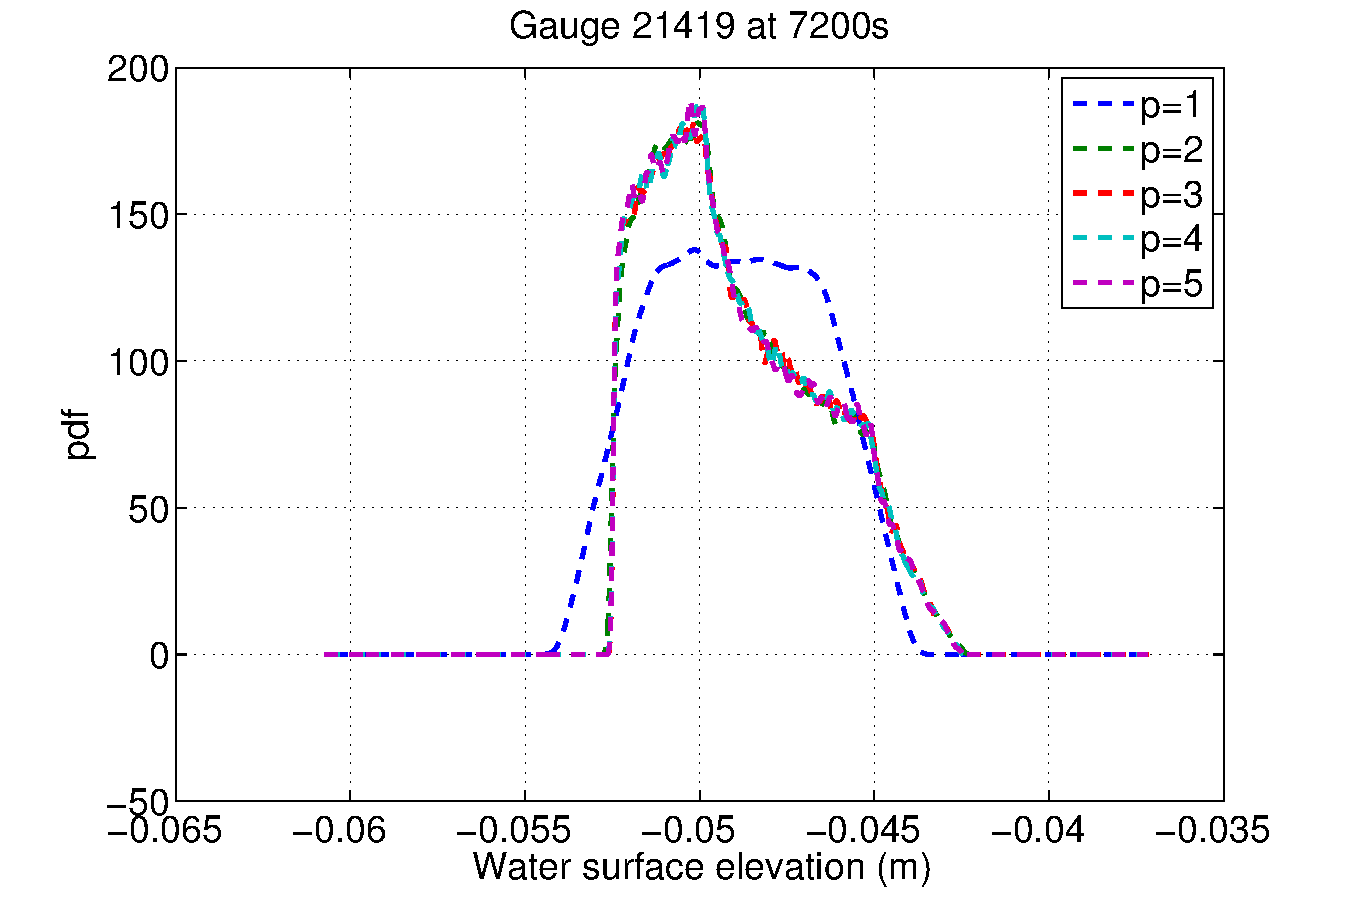
\includegraphics[width=0.5\textwidth]{./figures/pdfs4_2.pdf}
\end{tabular}
\caption{pdf of water surface elevation at the different gauge locations at t = 7200 s.}
\label{fig:pdfs2}
\end{figure}
%%%%%%%%%%%%%%%%%%%%%%%%%%%%%%%%%%%%%%%%%%%%%%%%%%%%%%%%%%%%%%%%
\begin{figure}[ht]
\centering
\begin{tabular}{clc}
        
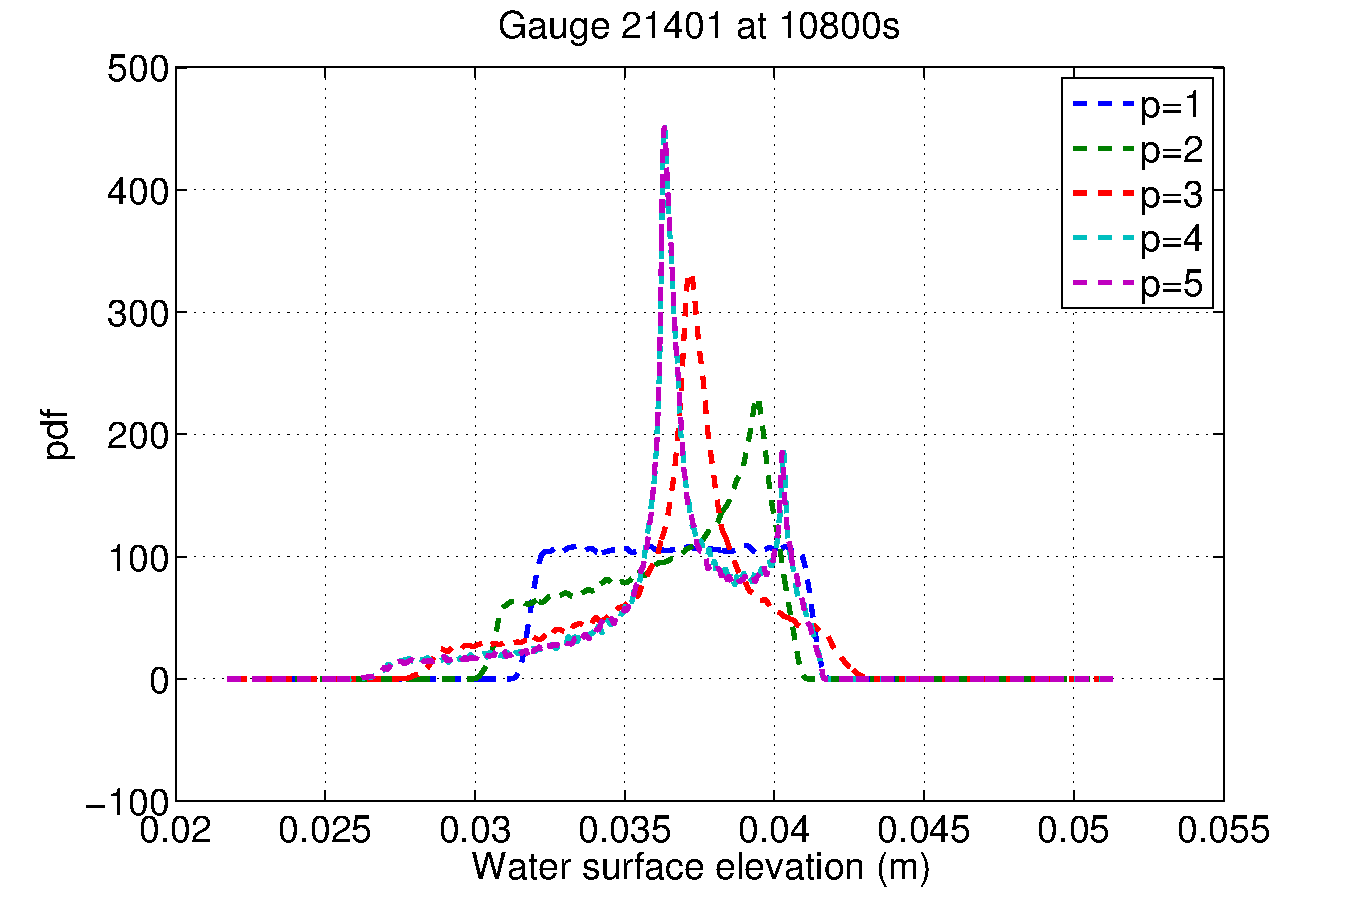
\includegraphics[width=0.5\textwidth]{./figures/pdfs1_3.pdf} &
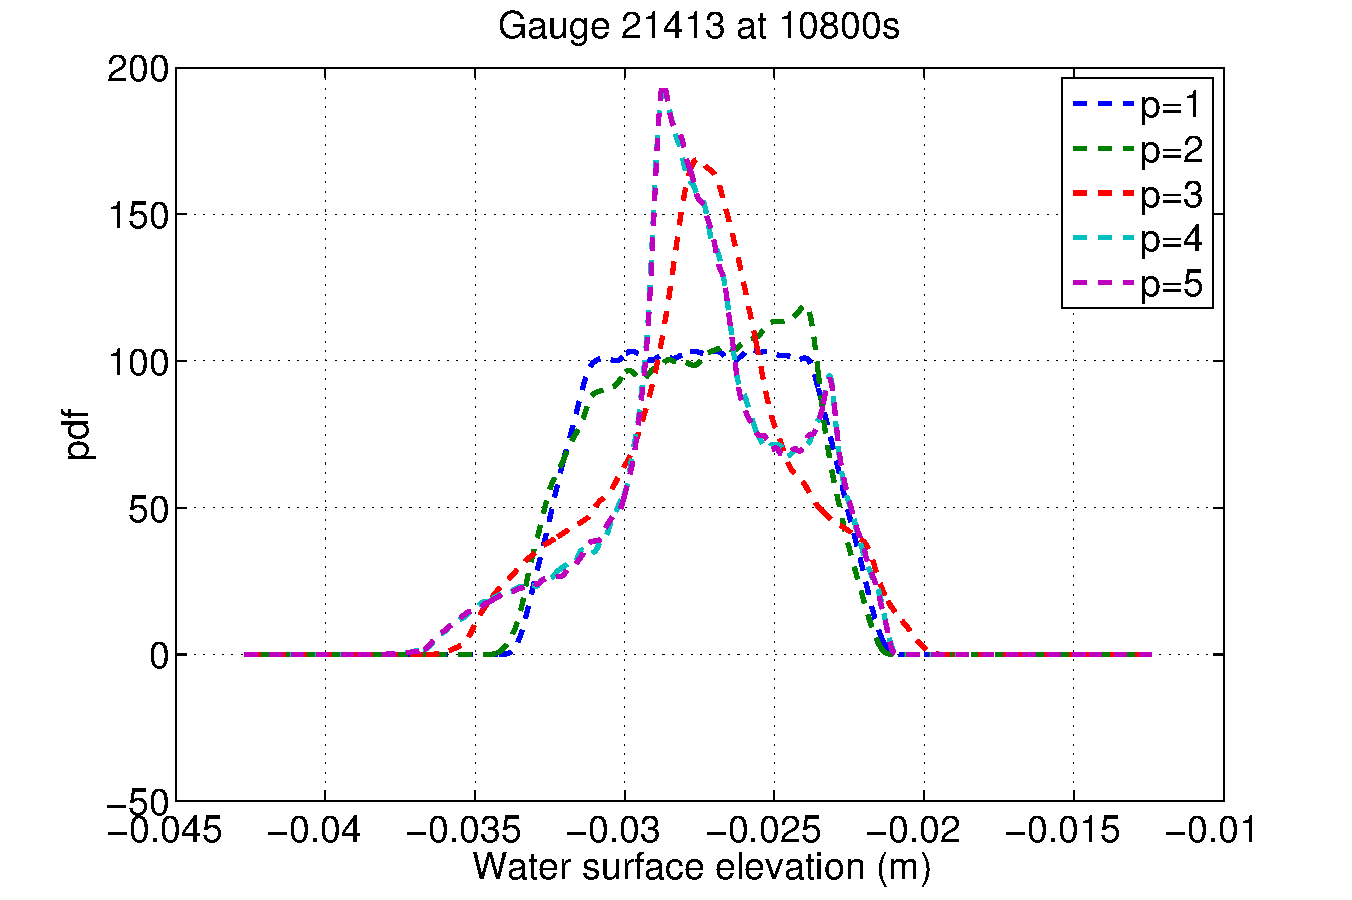
\includegraphics[width=0.5\textwidth]{./figures/pdfs2_3.pdf} \\
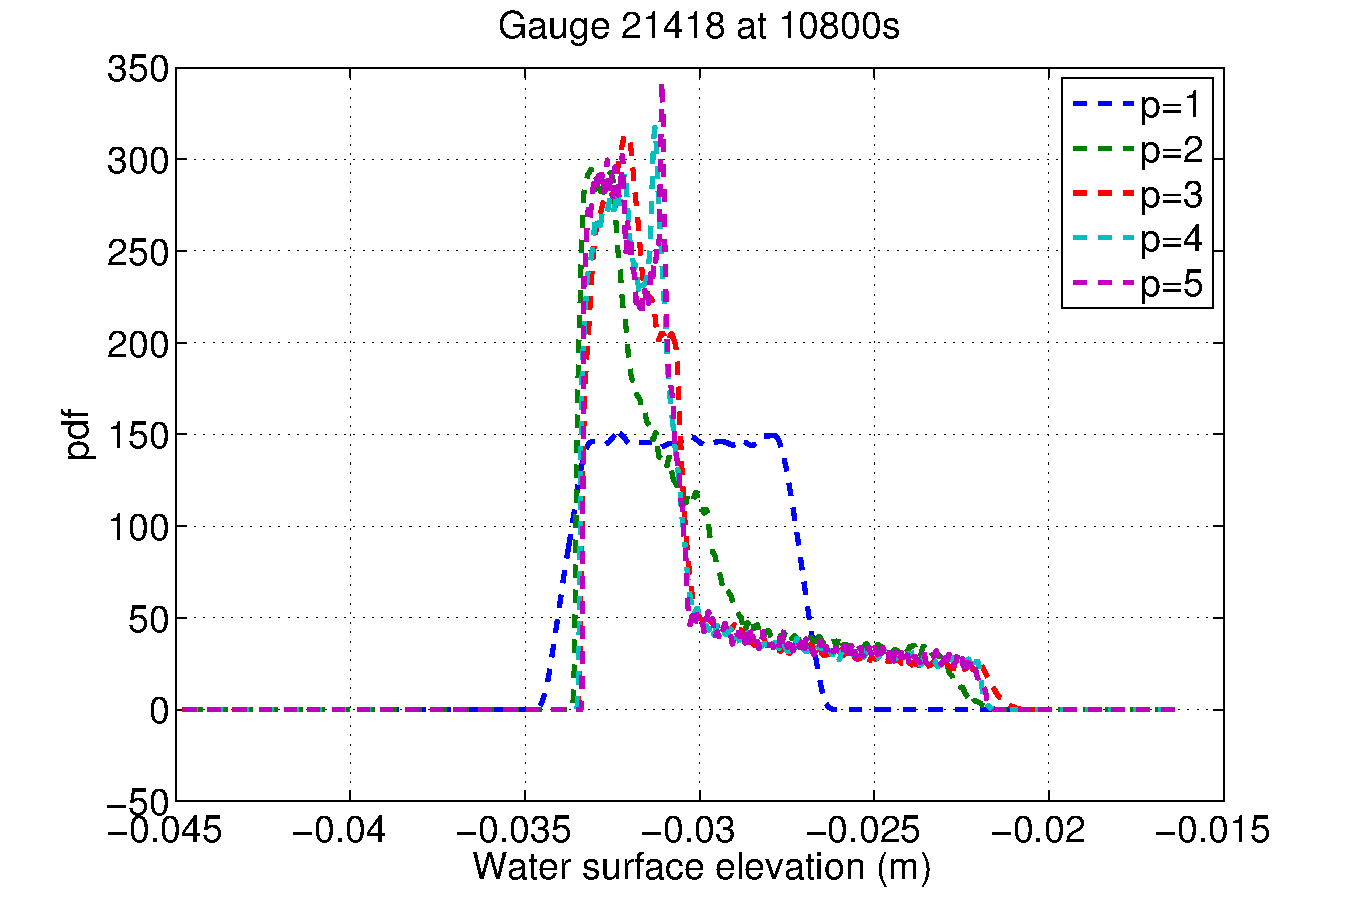
\includegraphics[width=0.5\textwidth]{./figures/pdfs3_3.pdf} &
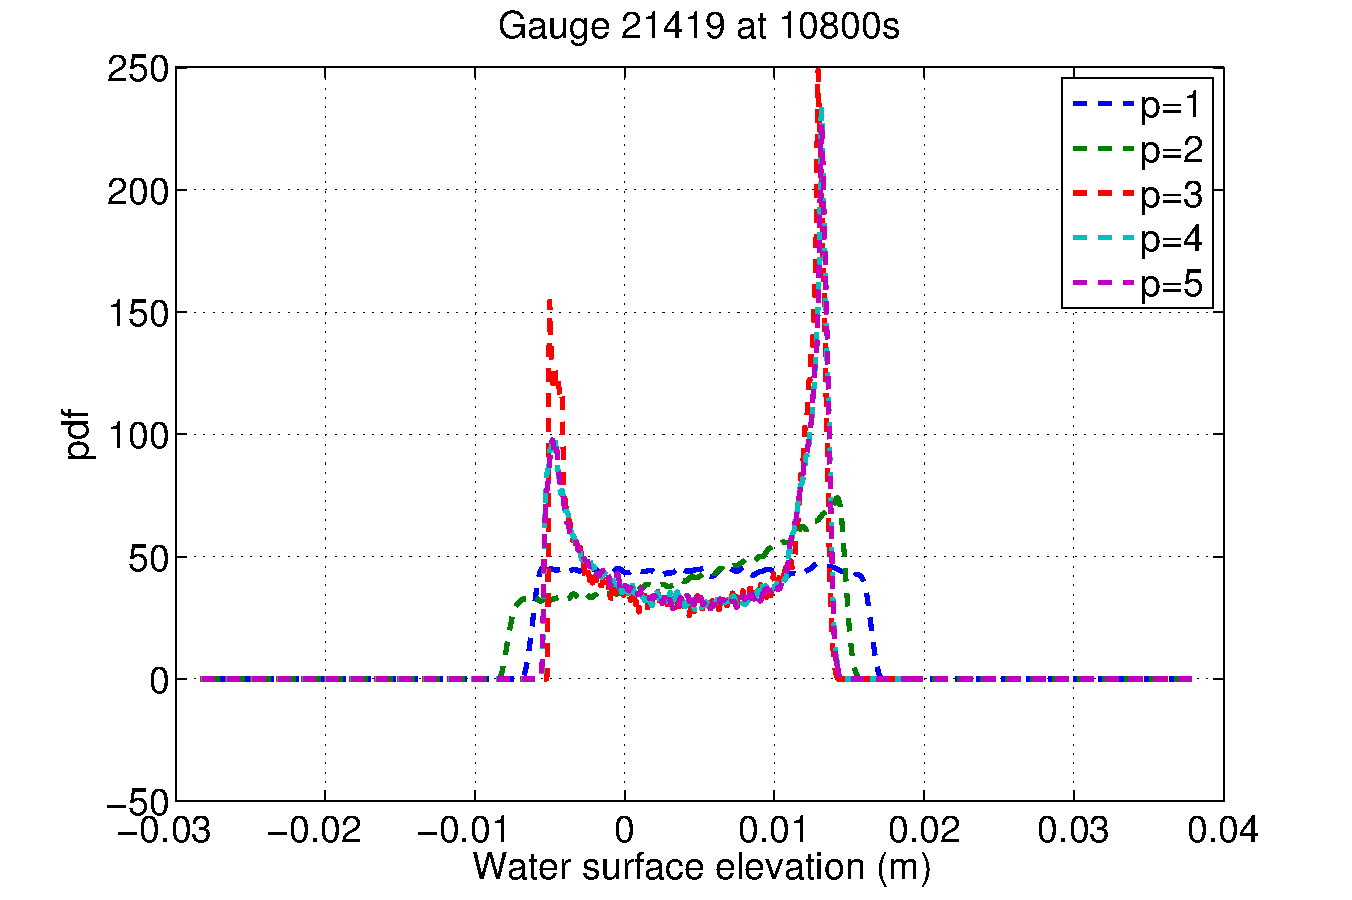
\includegraphics[width=0.5\textwidth]{./figures/pdfs4_3.pdf}
\end{tabular}
\caption{pdf of water surface elevation at the different gauge locations at t = 10800 s.}
\label{fig:pdfs3}
\end{figure}
%%%%%%%%%%%%%%%%%%%%%%%%%%%%%%%%%%%%%%%%%%%%%%%%%%%%%%%%%%%%%%%%
\begin{figure}[ht]
\begin{tabular}{clc}
        
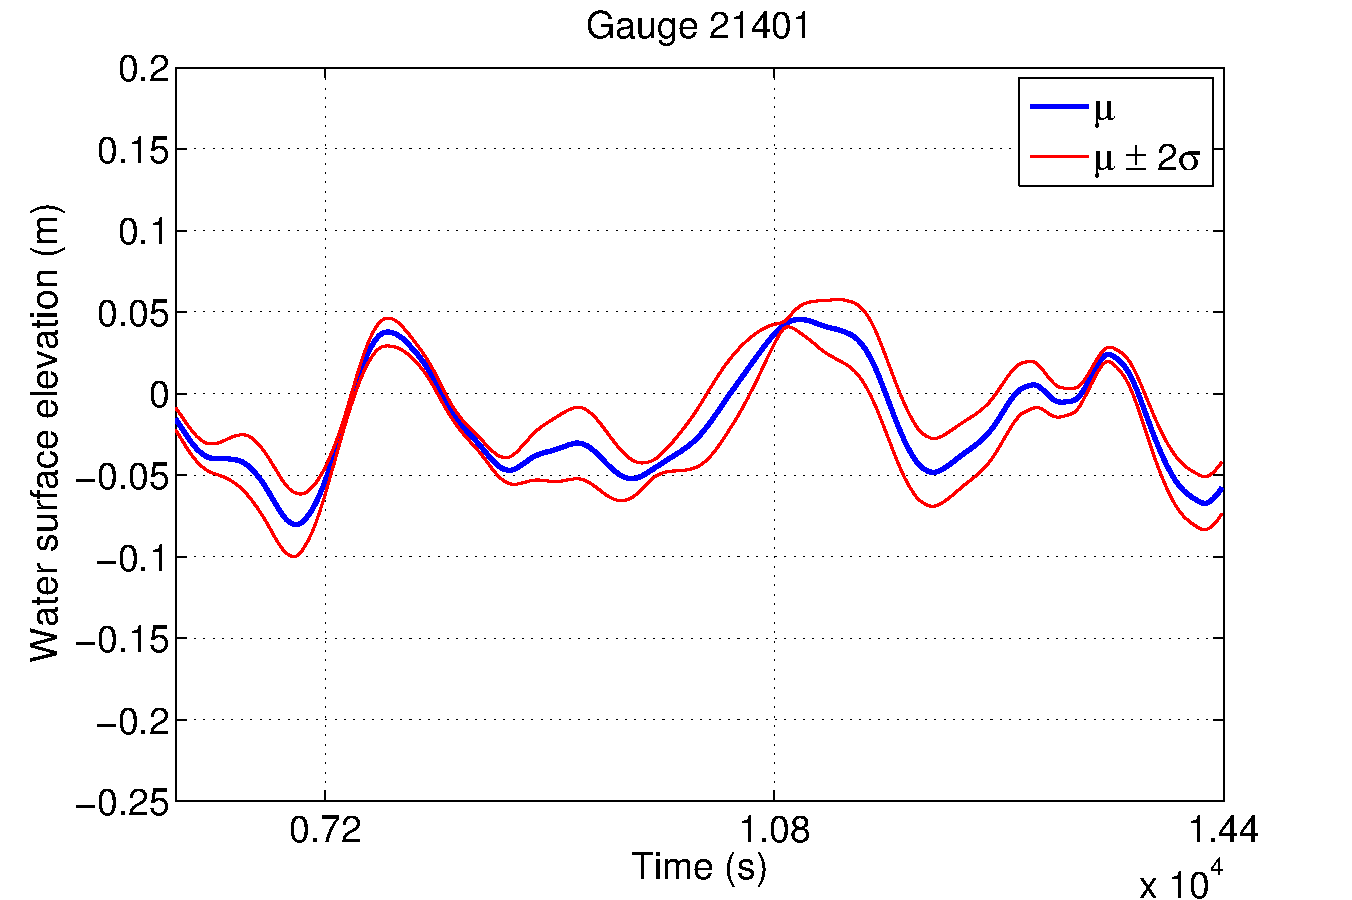
\includegraphics[width=0.475\textwidth]{./figures/musigma1.pdf} &
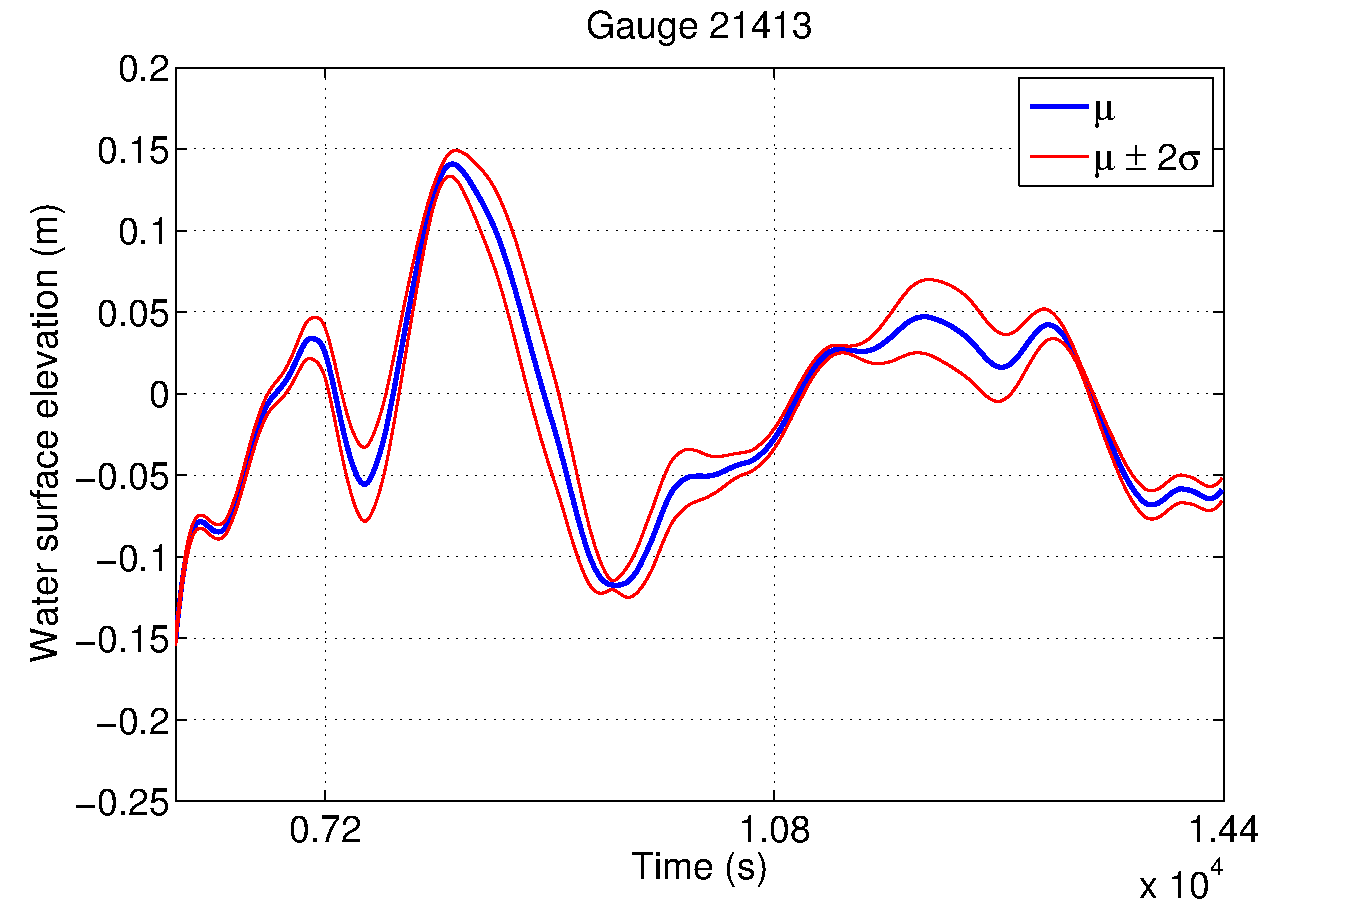
\includegraphics[width=0.475\textwidth]{./figures/musigma2.pdf} \\
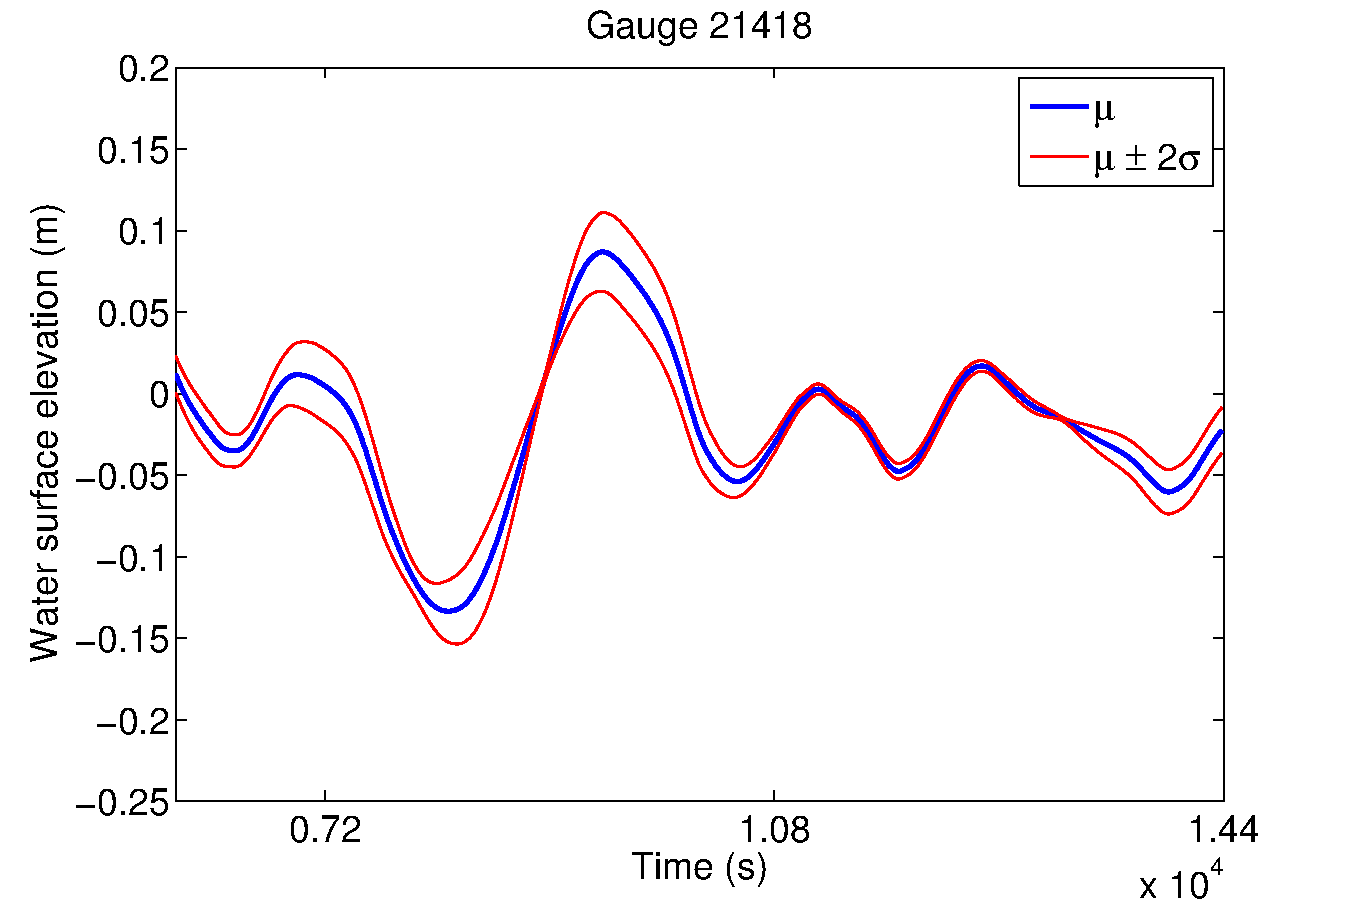
\includegraphics[width=0.475\textwidth]{./figures/musigma3.pdf} &
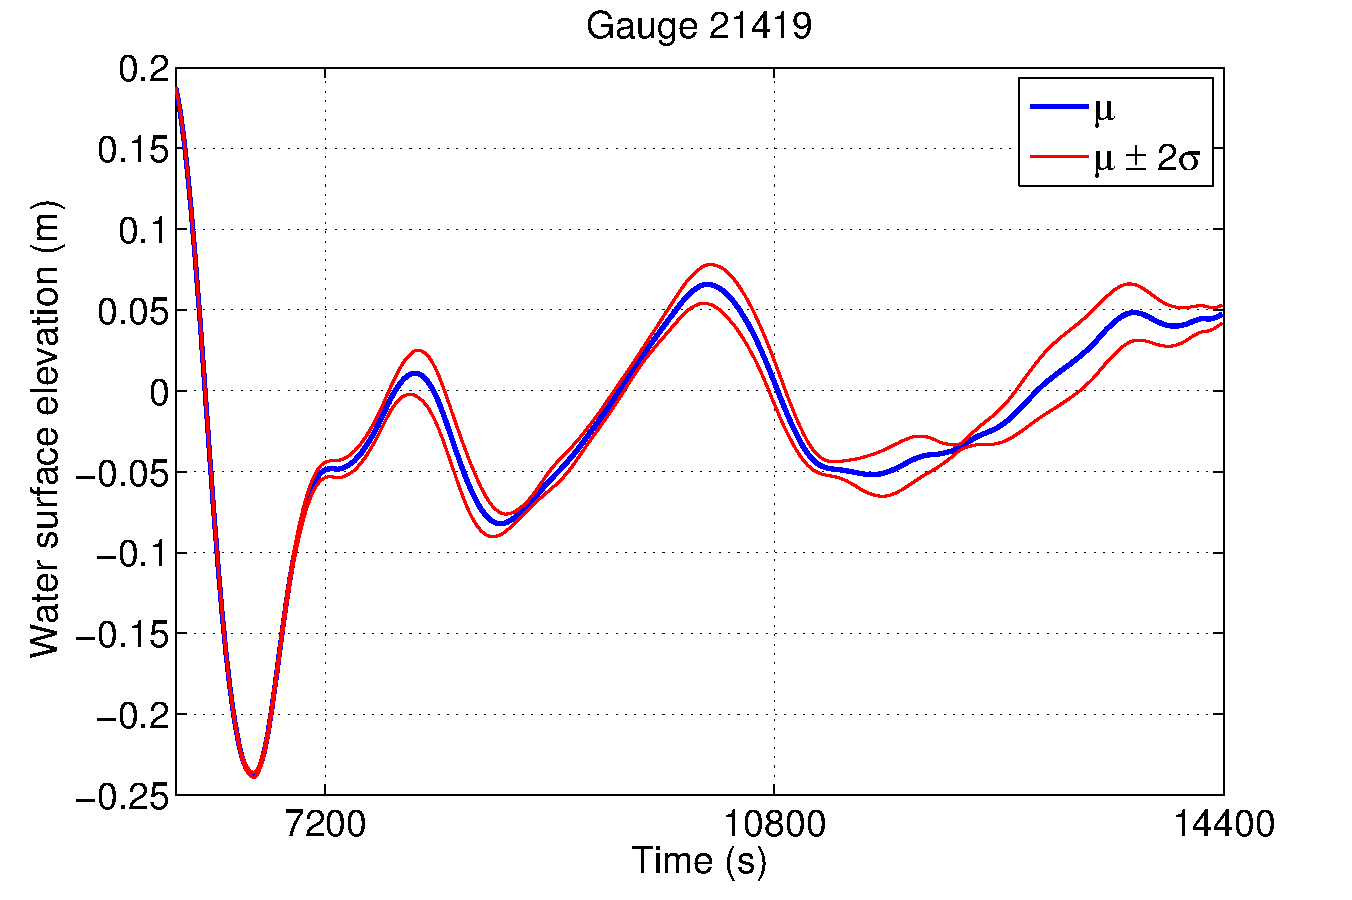
\includegraphics[width=0.475\textwidth]{./figures/musigma4.pdf}
\end{tabular}
\caption{Evolution of PC mean water surface elevation at different gauge locations.}
\label{fig:ave}
\end{figure}
%%%%%%%%%%%%%%%%%%%%%%%%%%%%%%%%%%%%%%%%%%%%%%%%%%%%%%%%%%%%%%%%
\begin{figure}[ht]
\begin{tabular}{clc}
%        
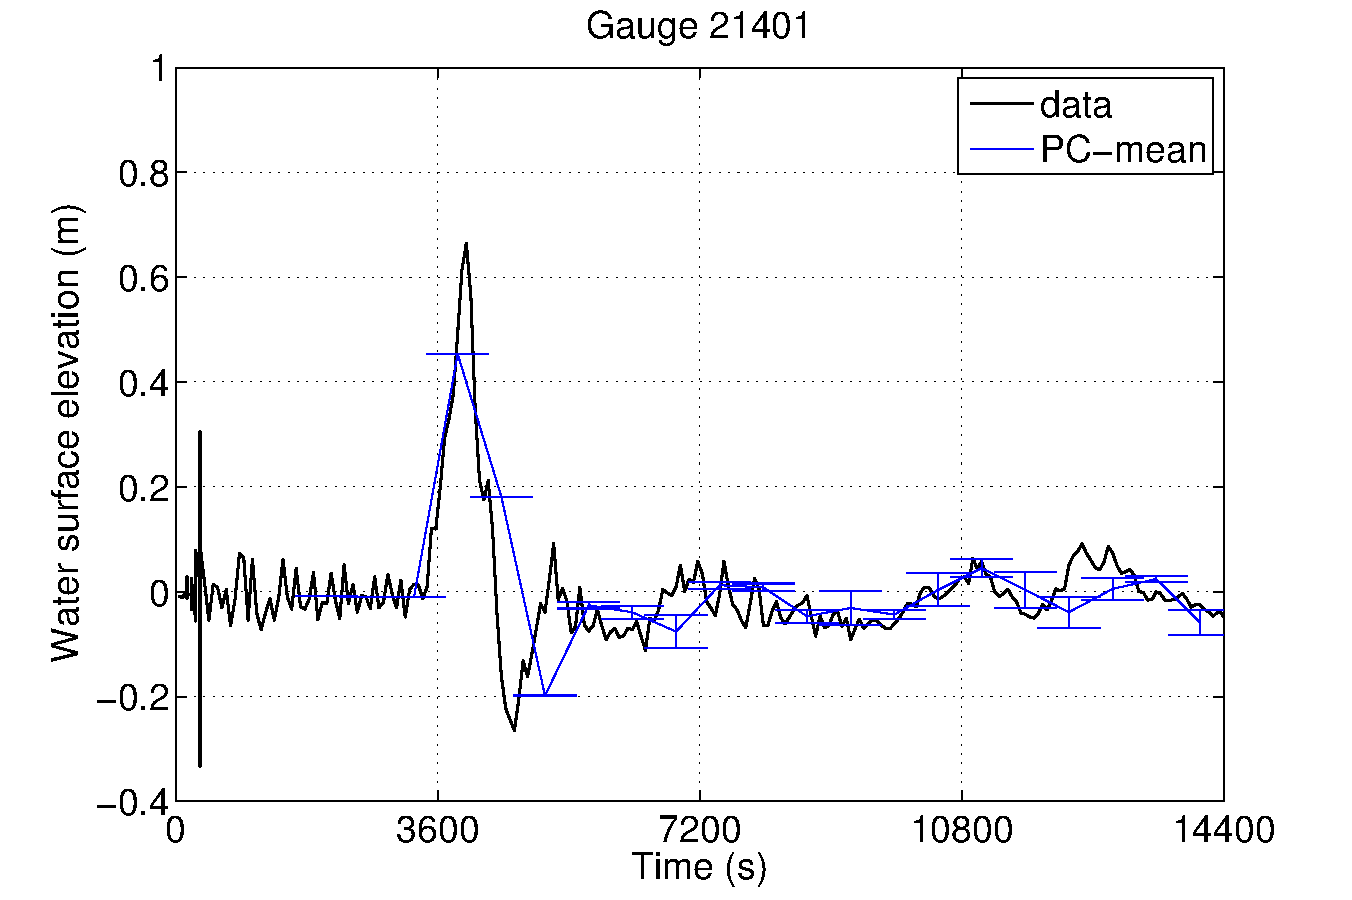
\includegraphics[width=0.475\textwidth]{./figures/compare1.pdf} &
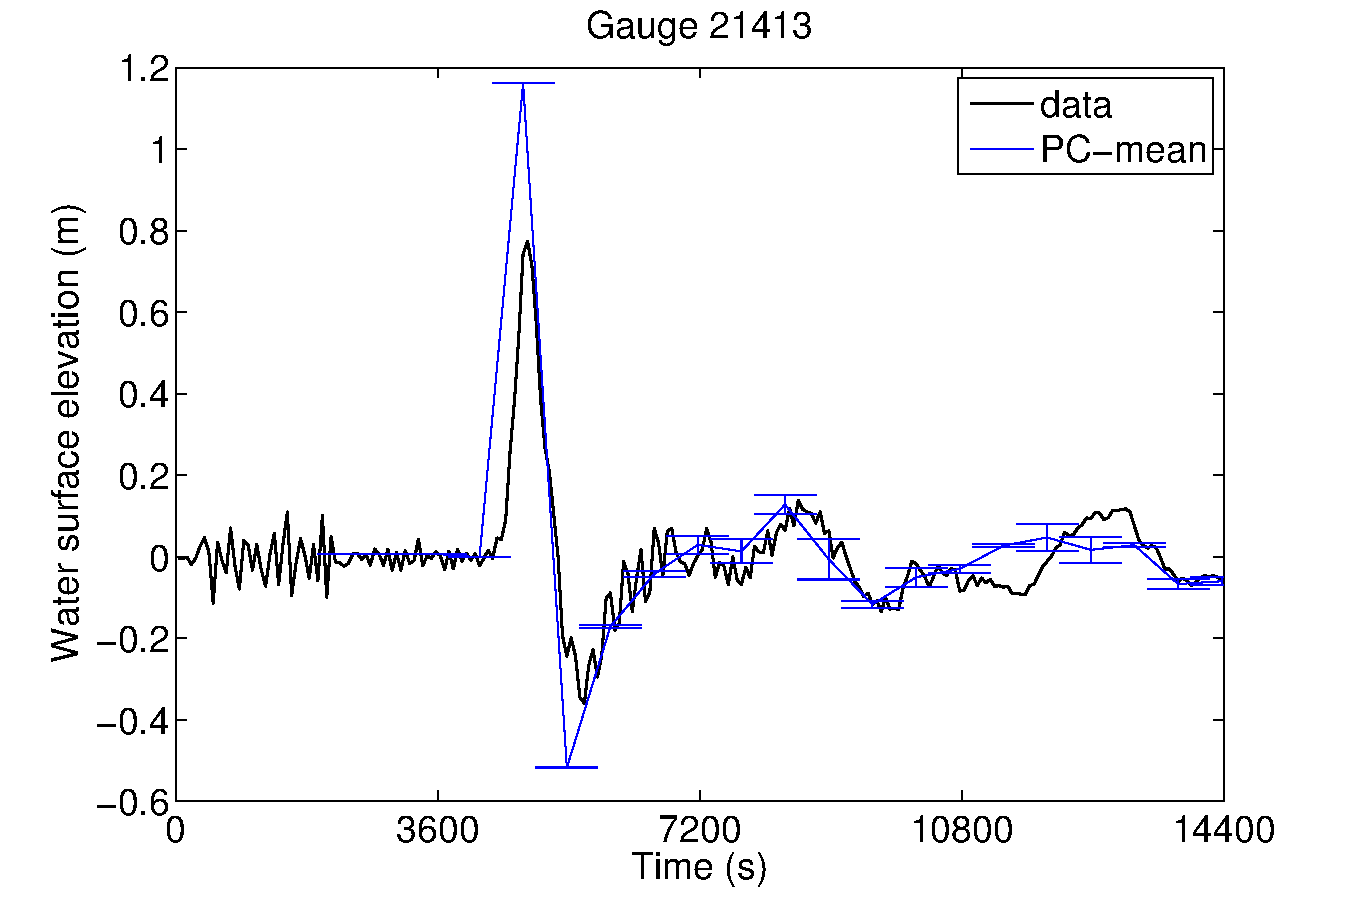
\includegraphics[width=0.475\textwidth]{./figures/compare2.pdf} \\
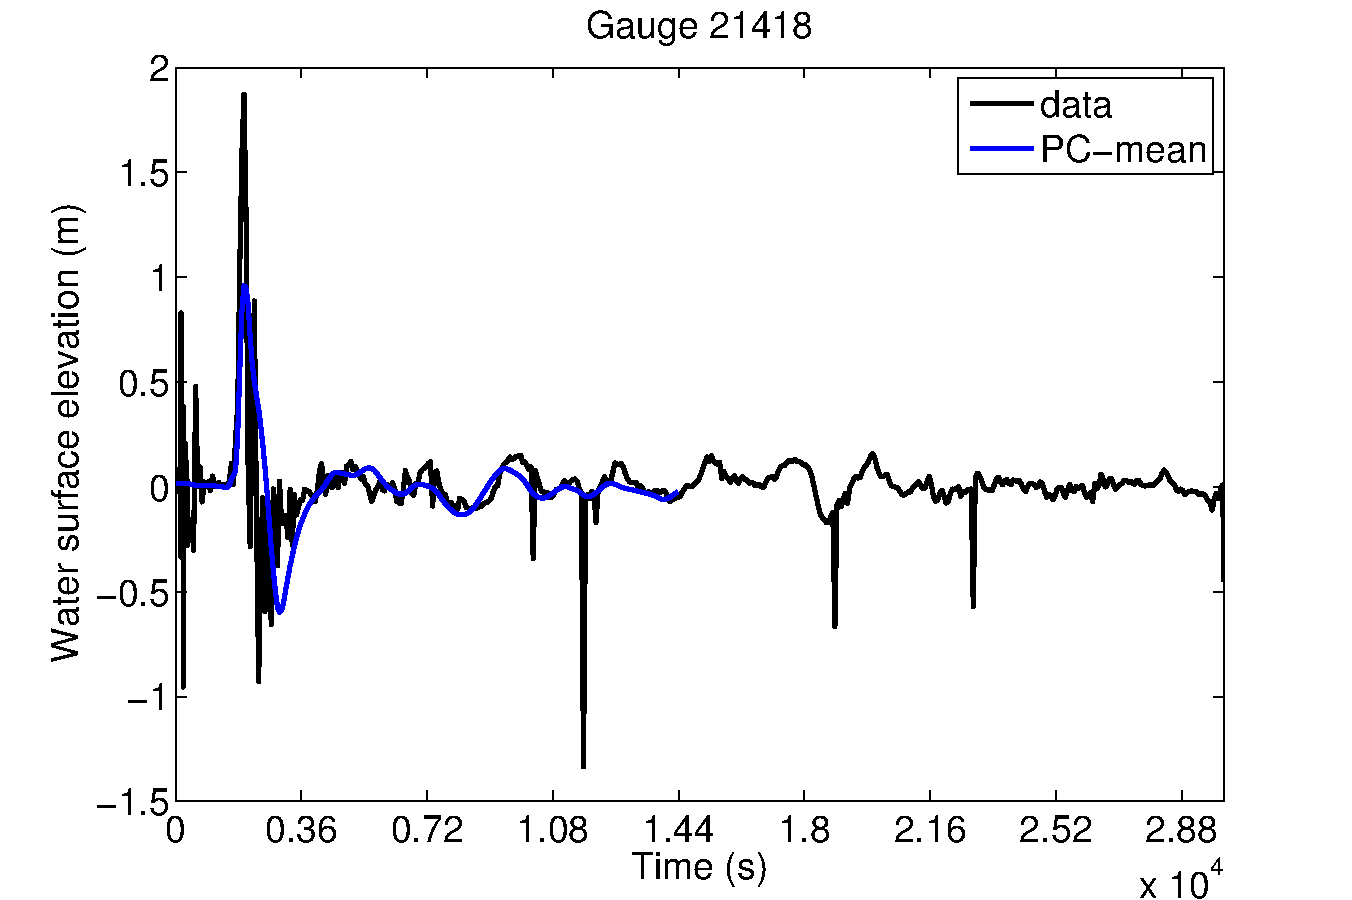
\includegraphics[width=0.475\textwidth]{./figures/compare3.pdf} &
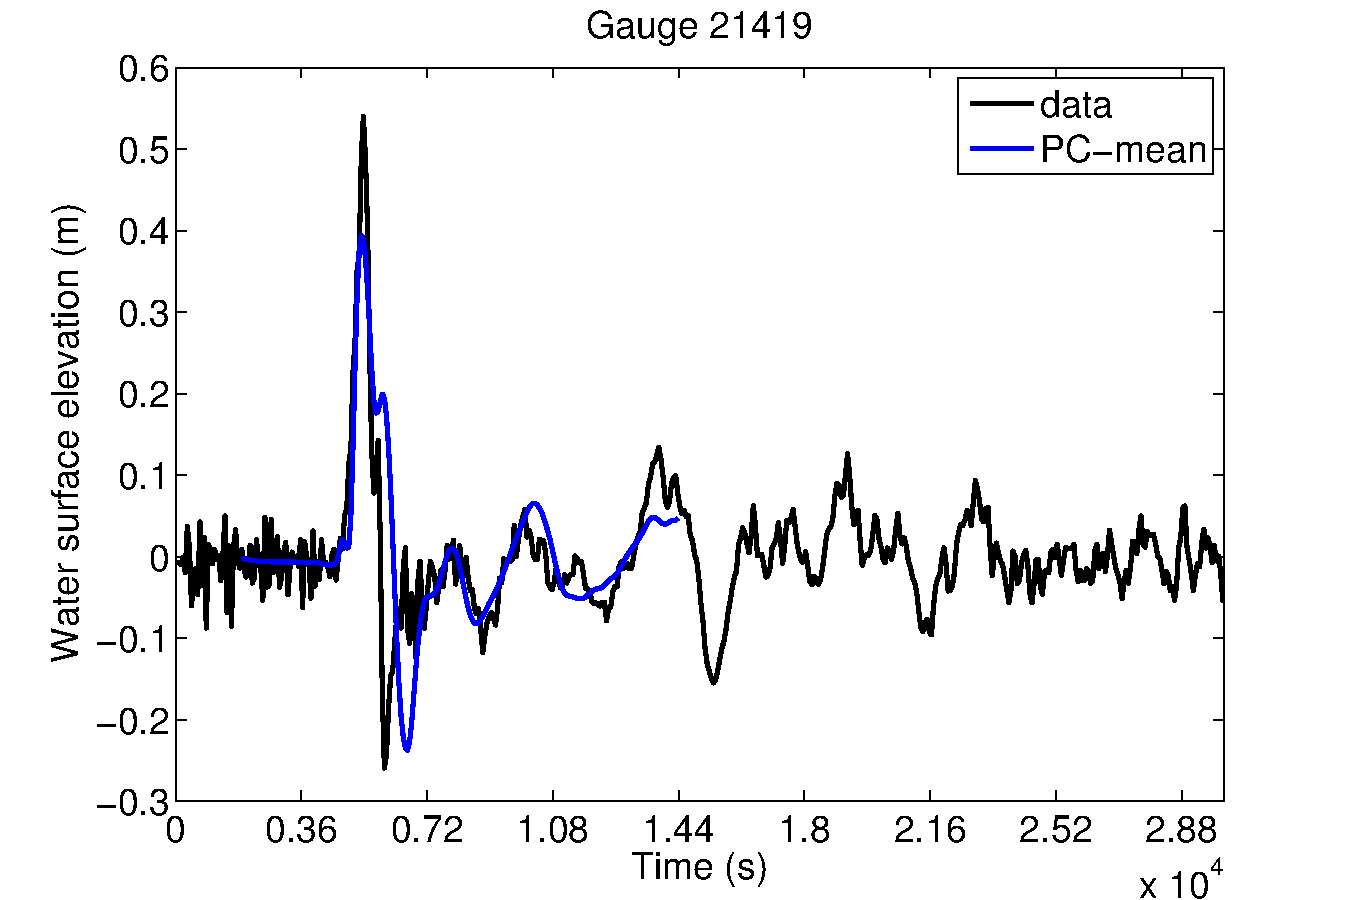
\includegraphics[width=0.475\textwidth]{./figures/compare4.pdf}
\end{tabular}
\caption{Comparison of PC mean 
and observed data of water surface elevation with time at the four gauges.}
\label{fig:compare}
\end{figure}  
%%%%%%%%%%%%%%%%%%%%%%%%%%%%%%%%%%%%%%%%%%%%%%%%%%%%%%%%%%%%%%%%
\begin{figure}[ht]
        \begin{tabular}{ccc}
\hspace*{-55pt}
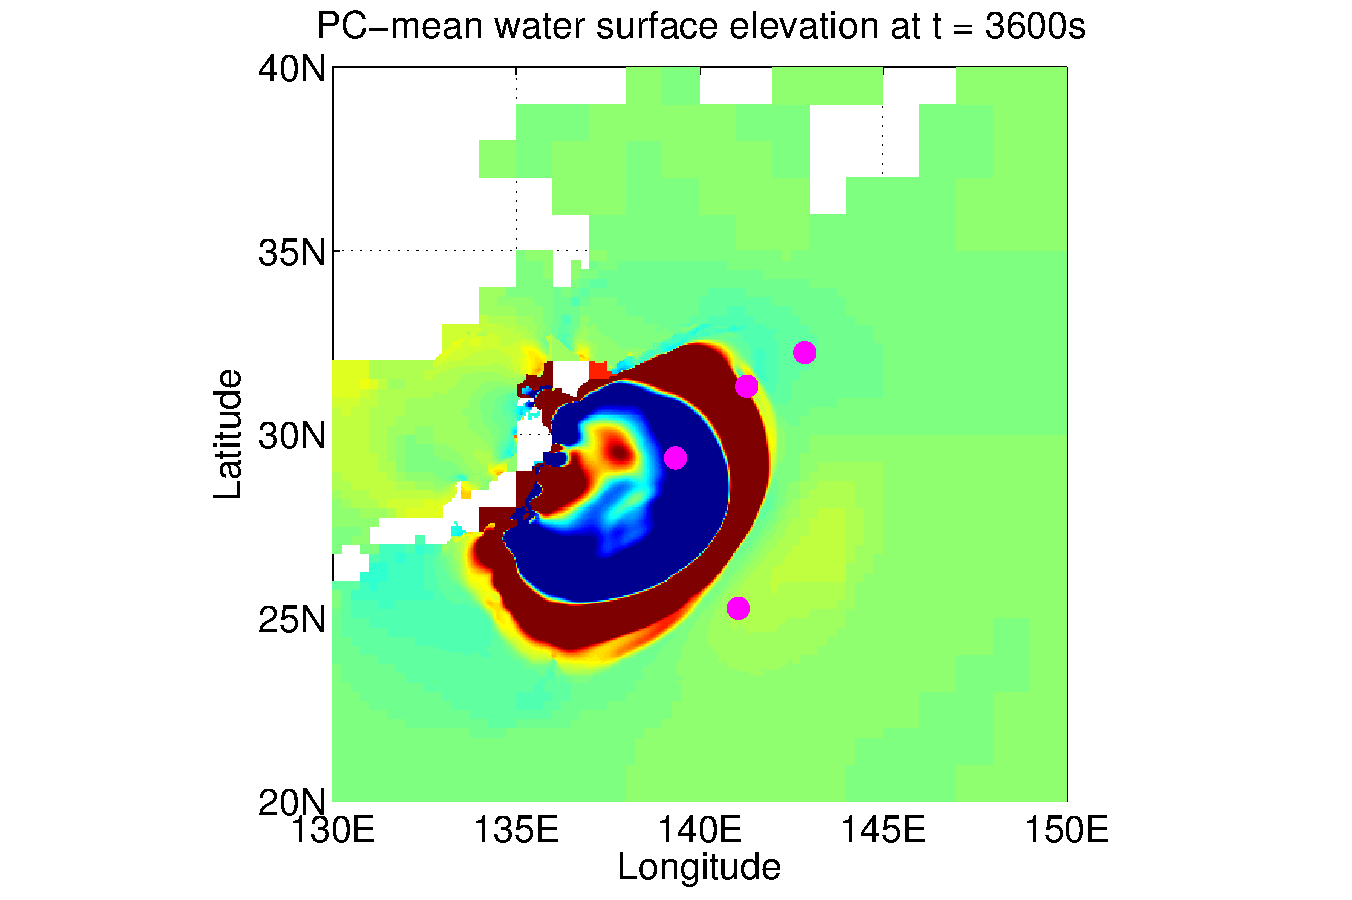
\includegraphics[width=0.45\textwidth]{./figures/mean2d1.pdf} &
\hspace*{-45pt}
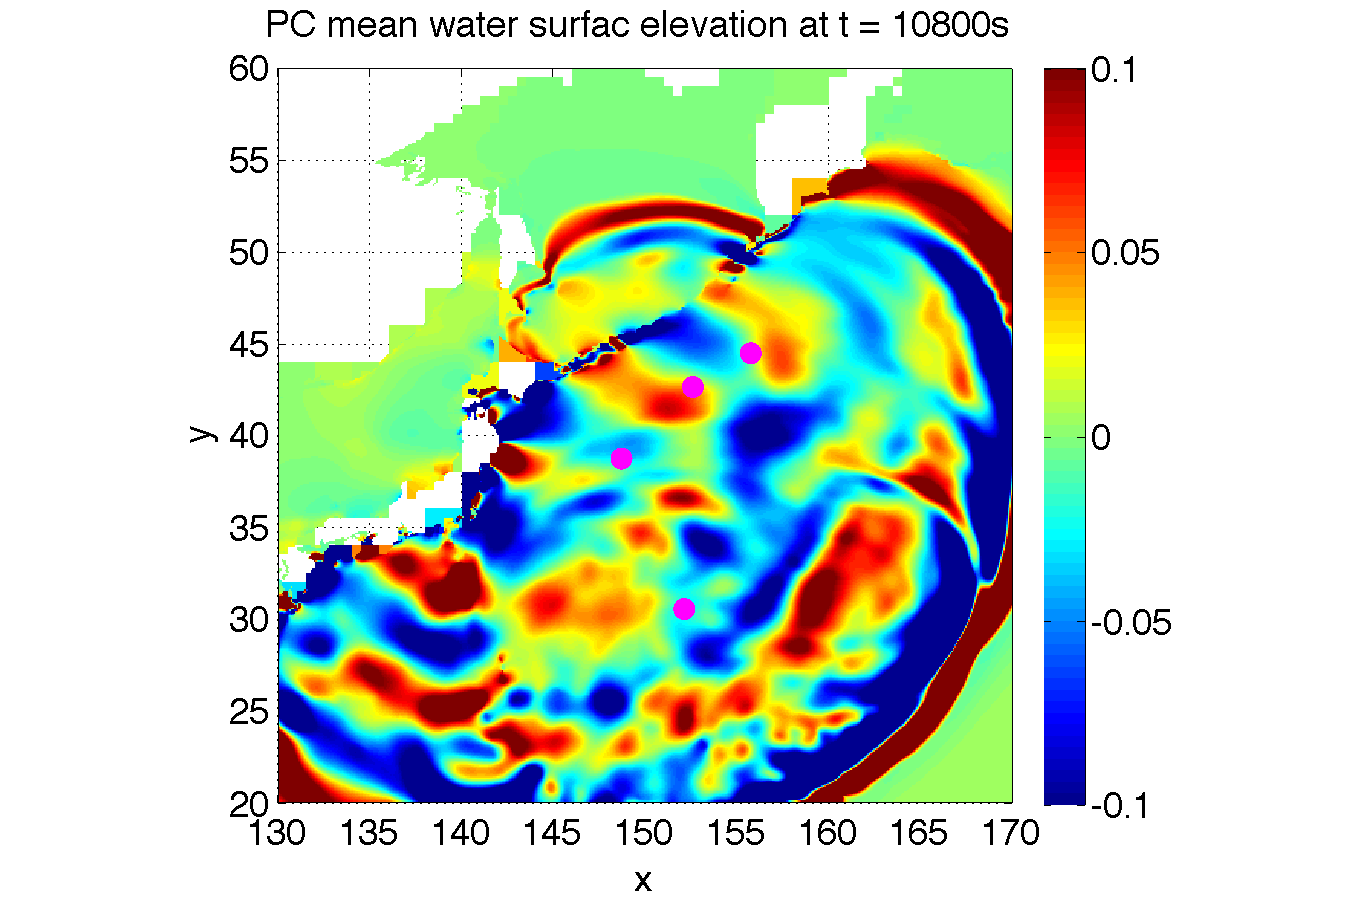
\includegraphics[width=0.45\textwidth]{./figures/mean2d3.pdf} &
\hspace*{-45pt}
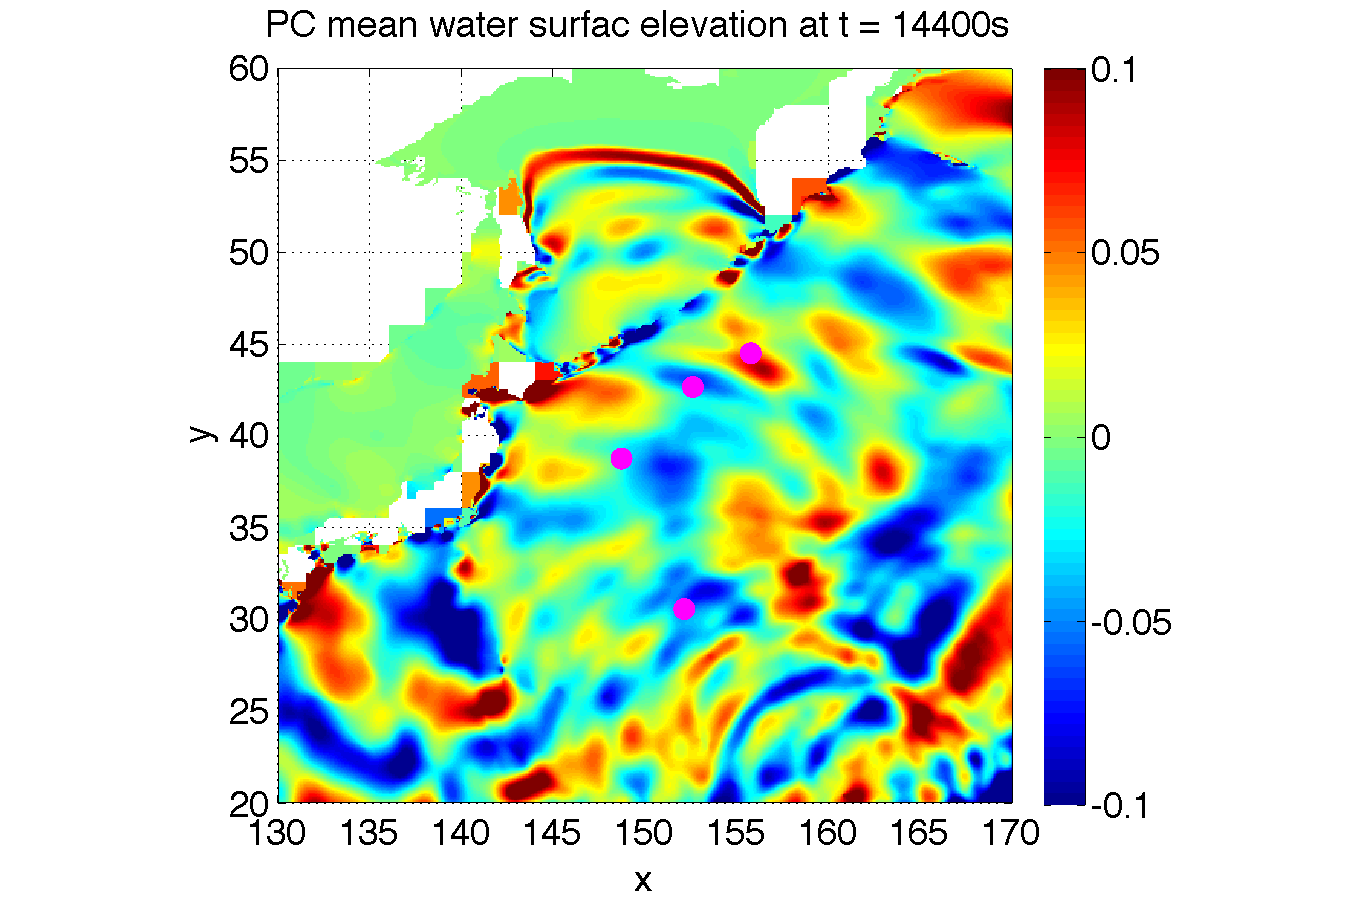
\includegraphics[width=0.45\textwidth]{./figures/mean2d4.pdf} \\
\hspace*{-55pt}
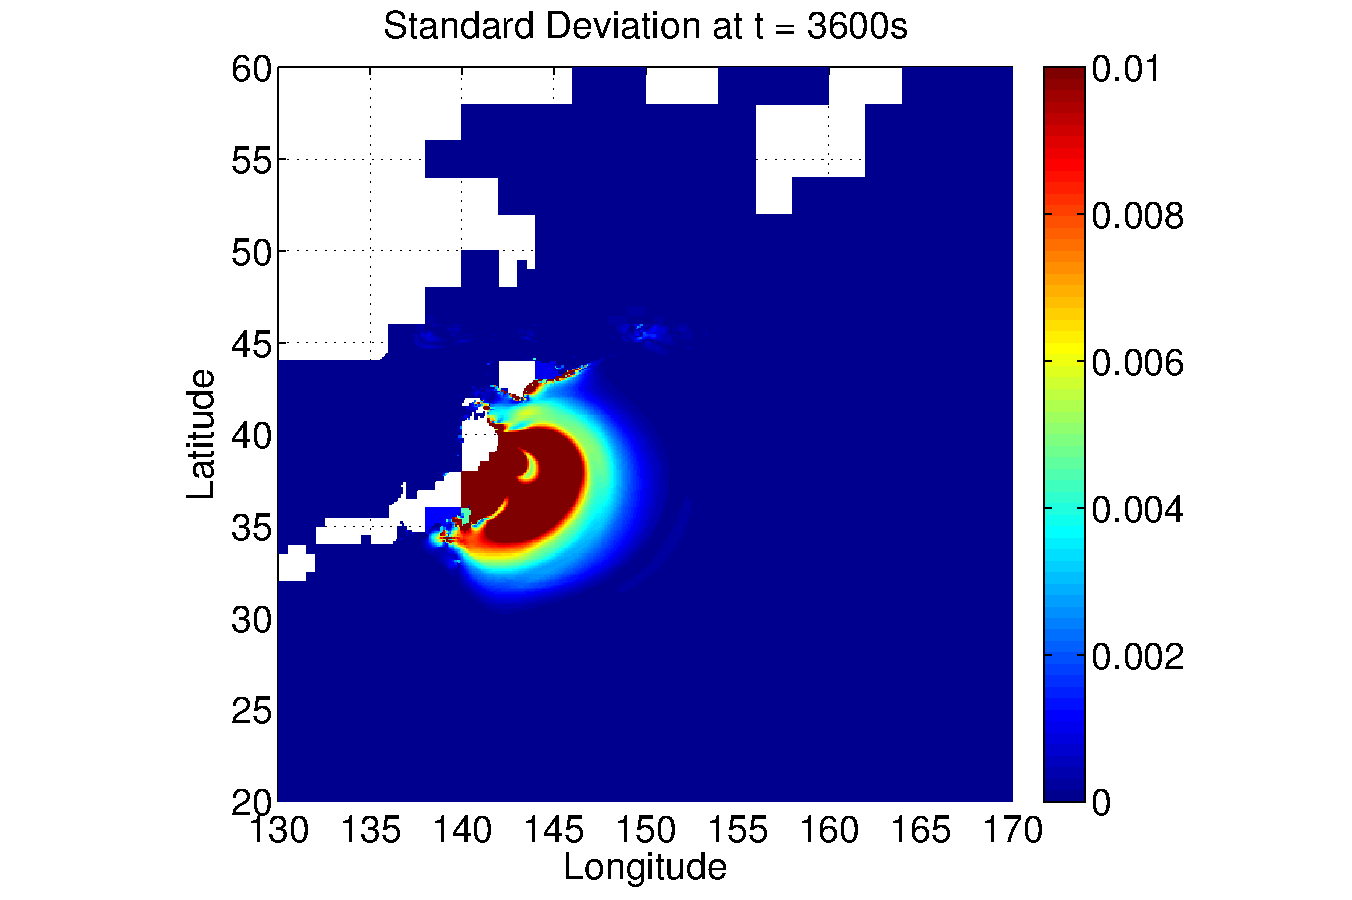
\includegraphics[width=0.45\textwidth]{./figures/sigma2d1.pdf} &
\hspace*{-45pt}
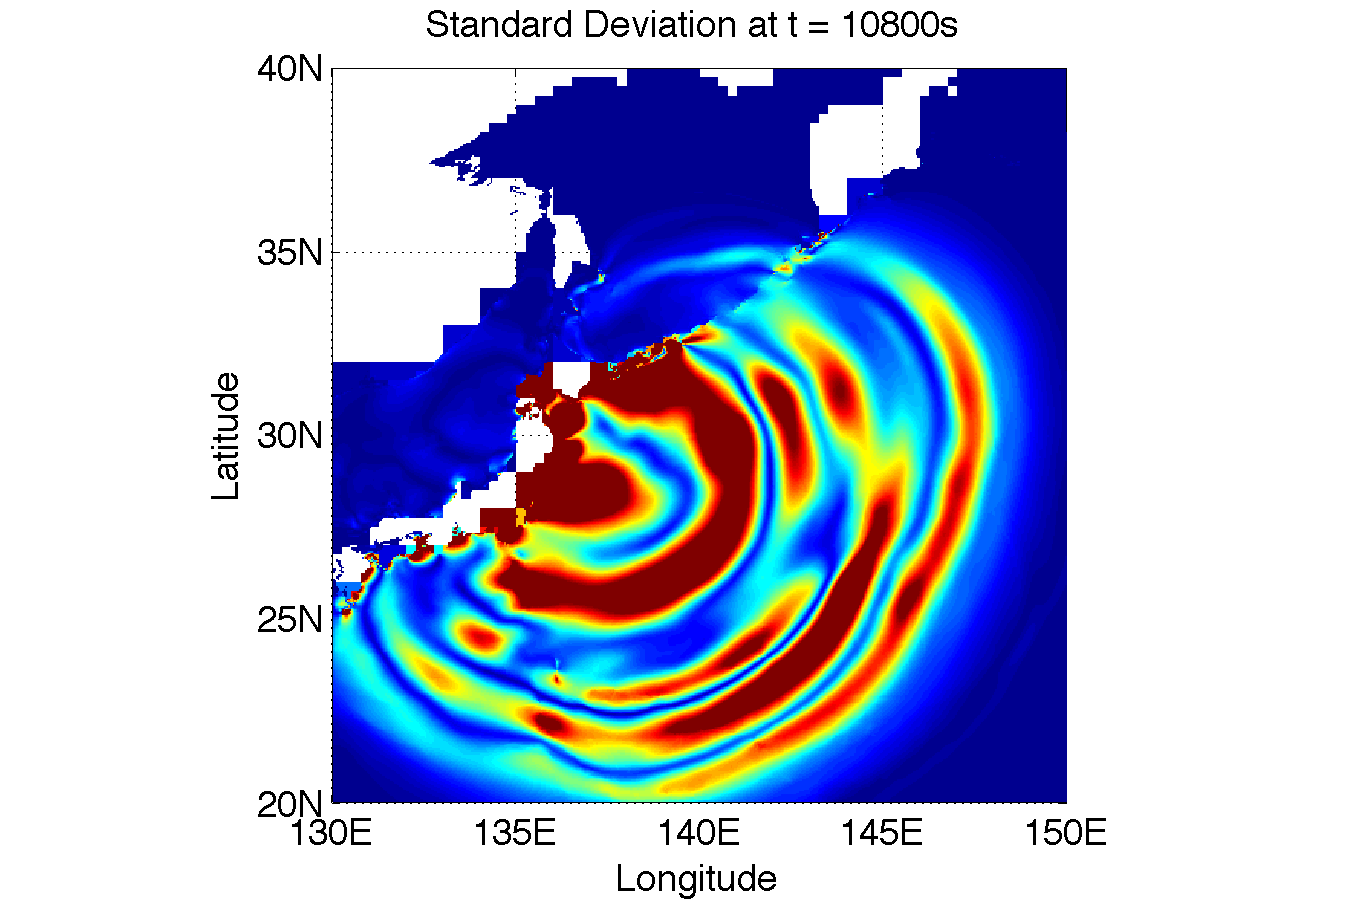
\includegraphics[width=0.45\textwidth]{./figures/sigma2d3.pdf} &
\hspace*{-45pt}
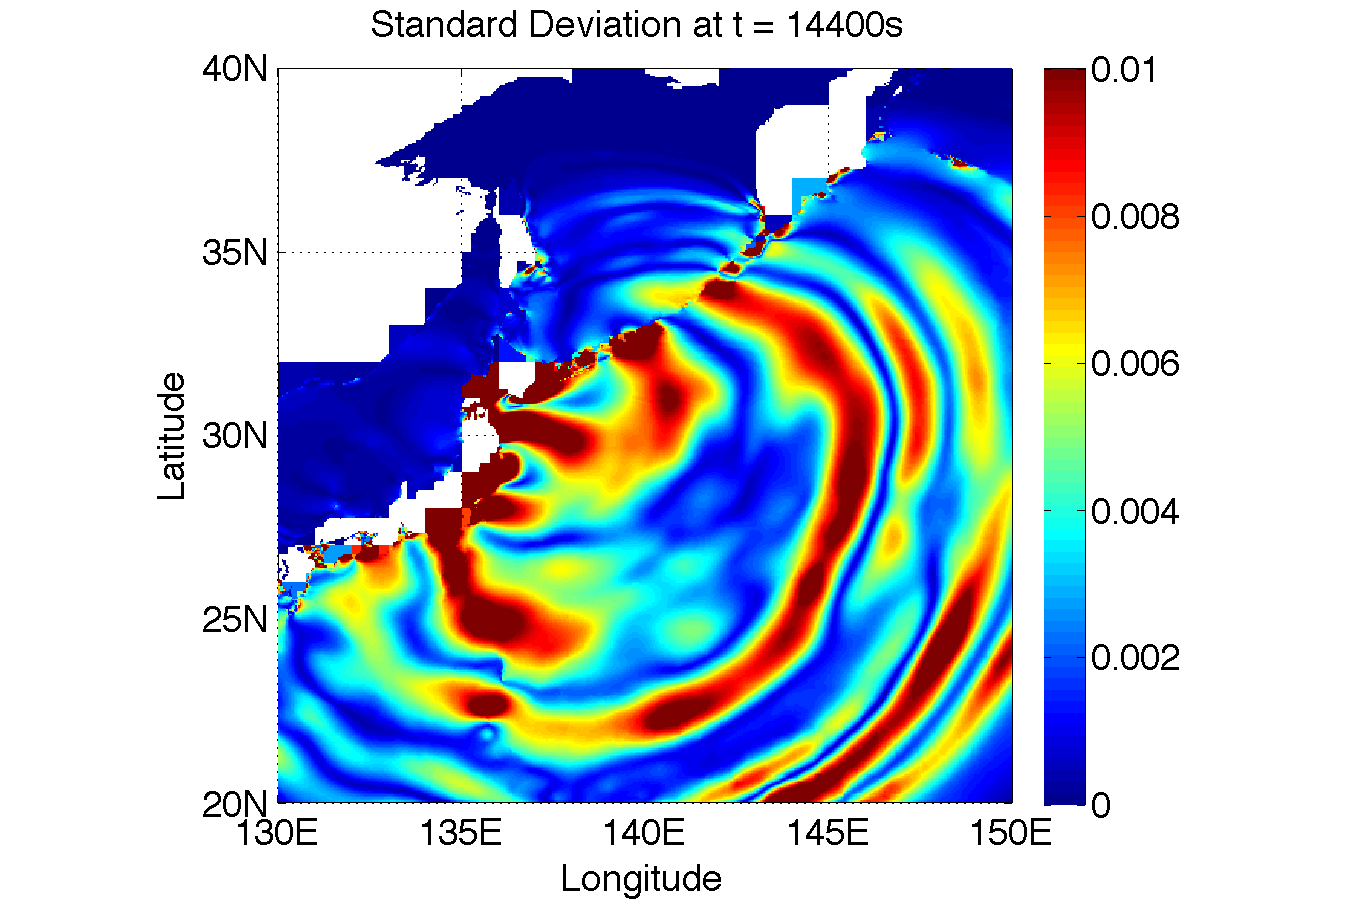
\includegraphics[width=0.45\textwidth]{./figures/sigma2d4.pdf}
\end{tabular}
\caption{PC mean (top row) and standard deviation (bottom row) of the water surface elevation at different times.}
\label{fig:mean2d}
\end{figure}
%%%%%%%%%%%%%%%%%%%%%%%%%%%%%%%%%%%%%%%%%%%%%%%%%%%%%%%%%%%%%%%%

\begin{figure}[ht]
\begin{tabular}{clc}
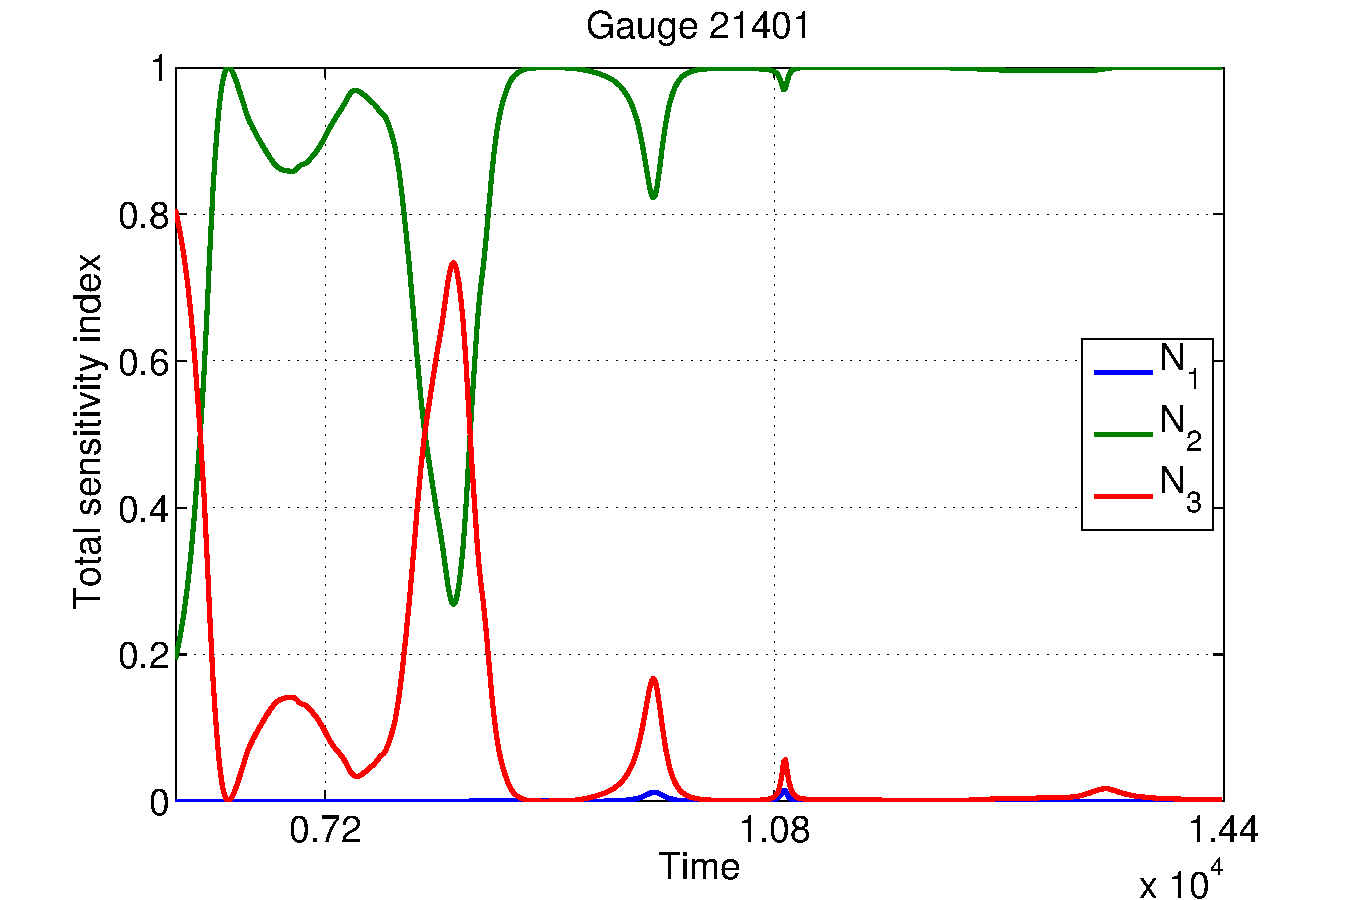
\includegraphics[width=0.475\textwidth]{./figures/sens1.pdf} &
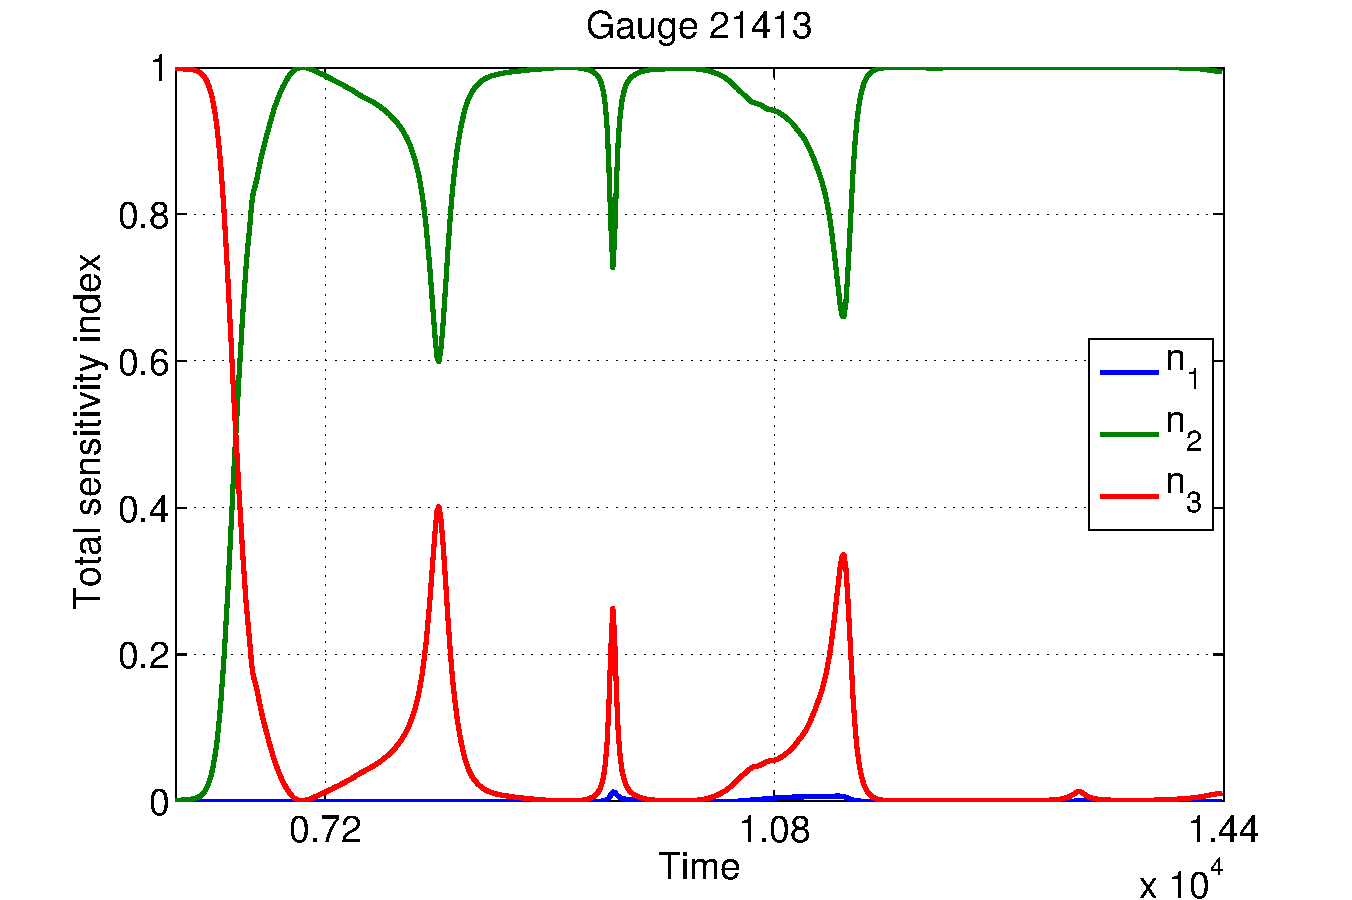
\includegraphics[width=0.475\textwidth]{./figures/sens2.pdf} \\
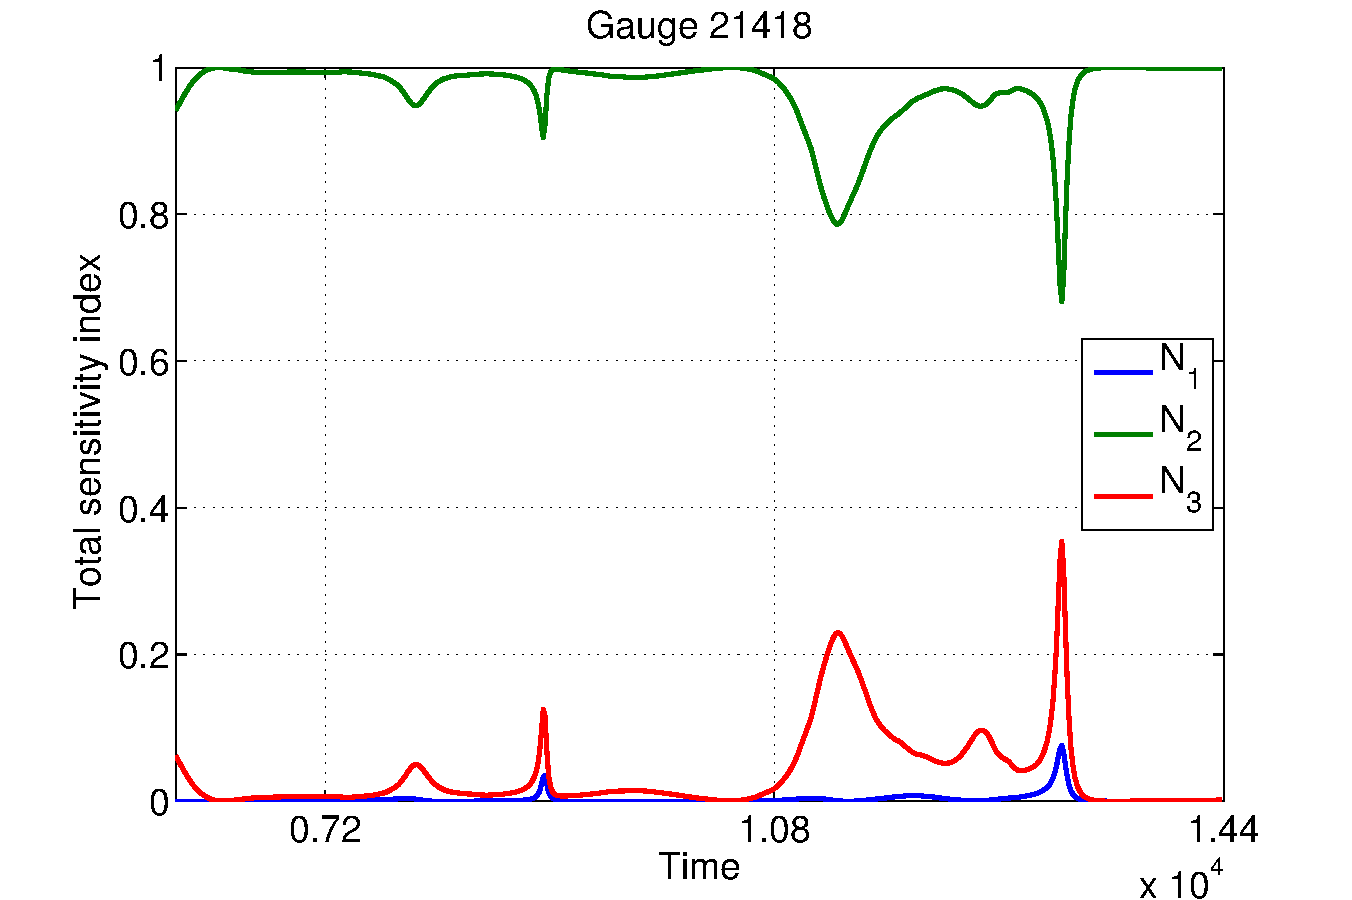
\includegraphics[width=0.475\textwidth]{./figures/sens3.pdf} &
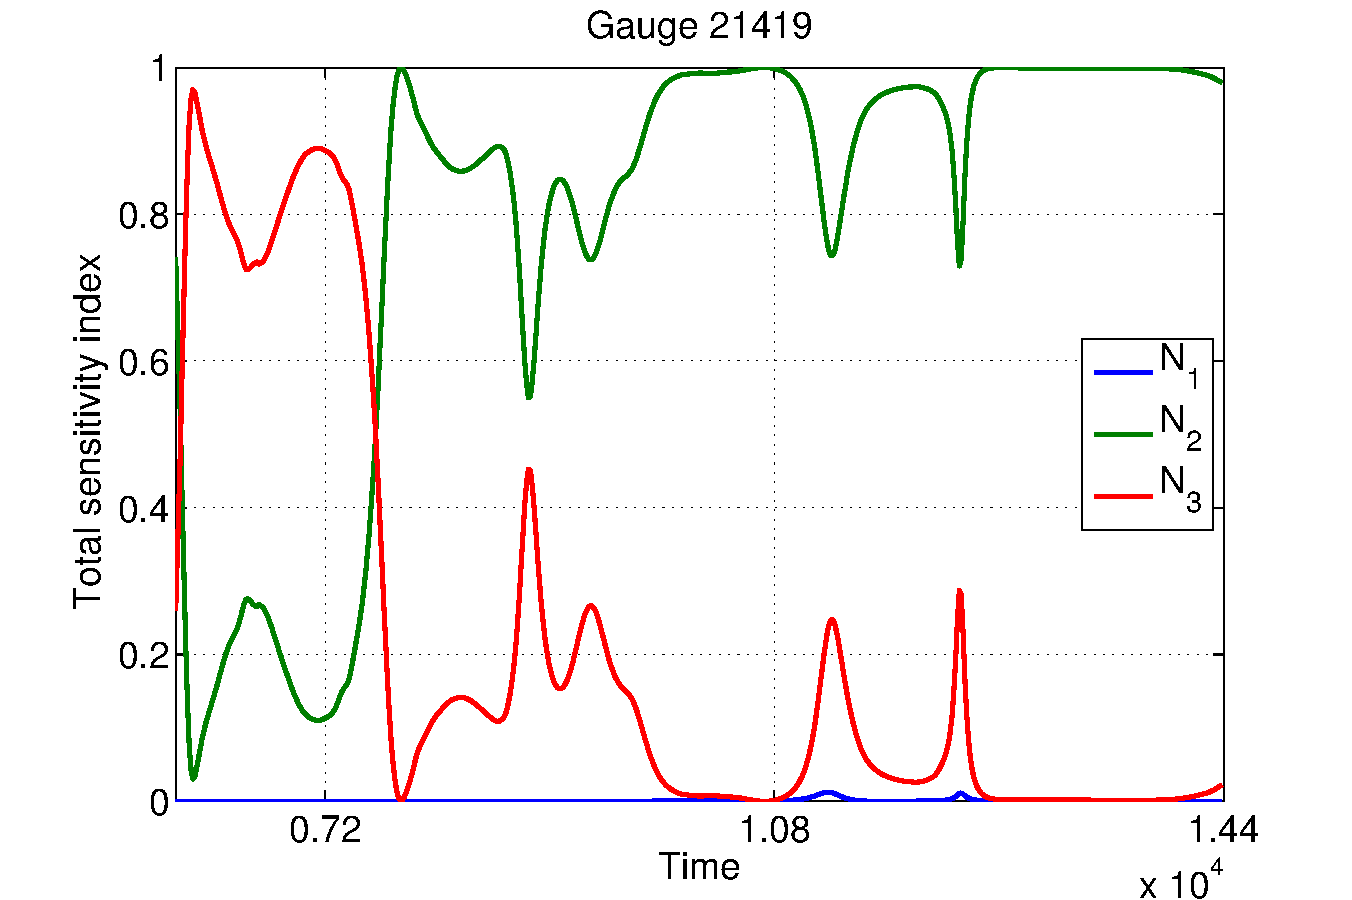
\includegraphics[width=0.475\textwidth]{./figures/sens4.pdf}
\end{tabular}
\caption{Total sensitivity index of different input parameters.}
\label{fig:sens}
\end{figure}
%%%%%%%%%%%%%%%%%%%%%%%%%%%%%%%%%%%%%%%%%%%%%%%%%%%%%%%%%%%%%%%%

\begin{figure}[ht]
\begin{tabular}{clc}
 \hspace*{-55pt}
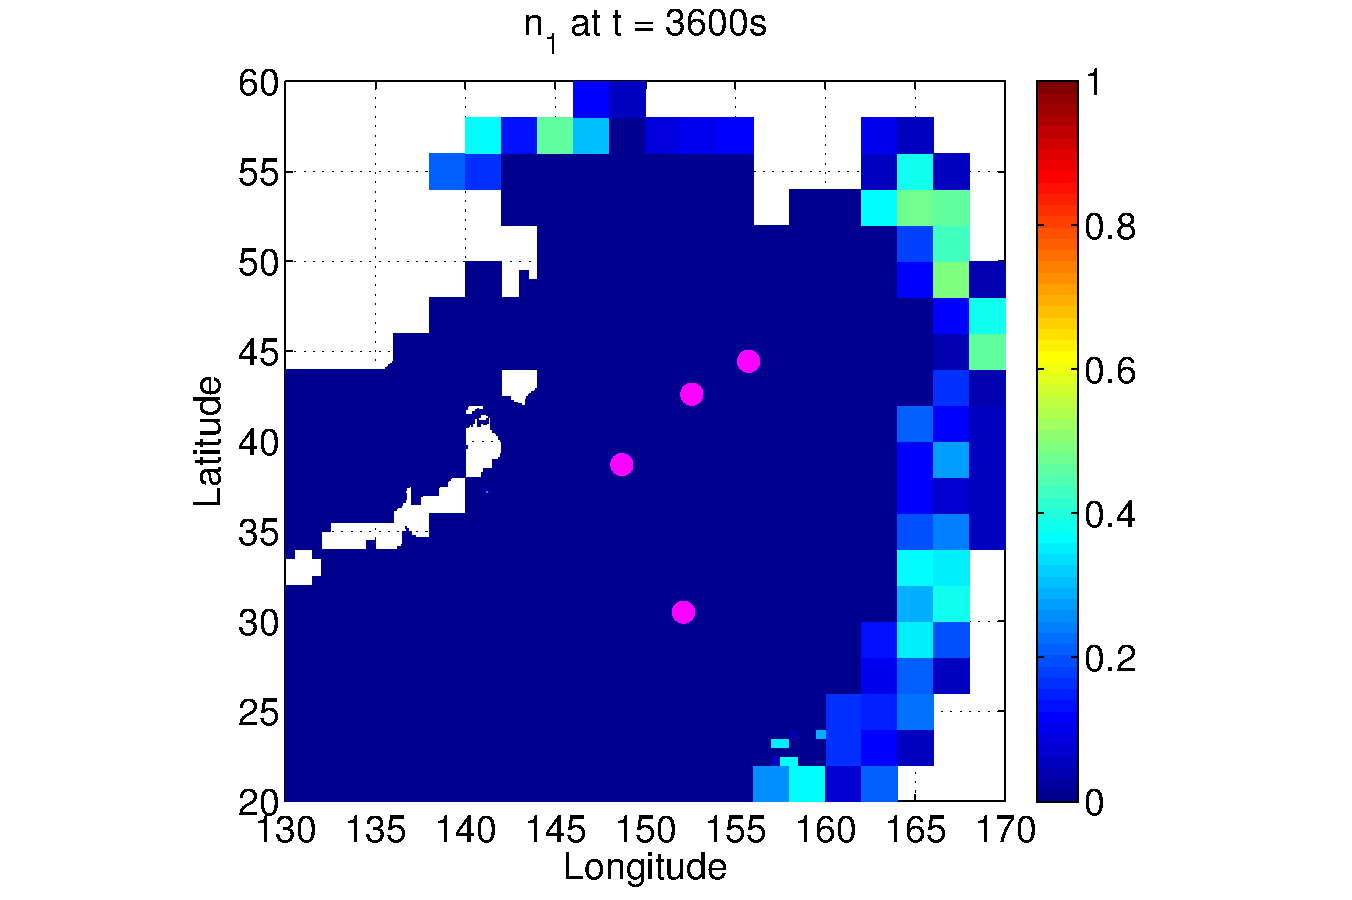
\includegraphics[width=0.45\textwidth]{./figures/T12d1.pdf} &
\hspace*{-45pt}
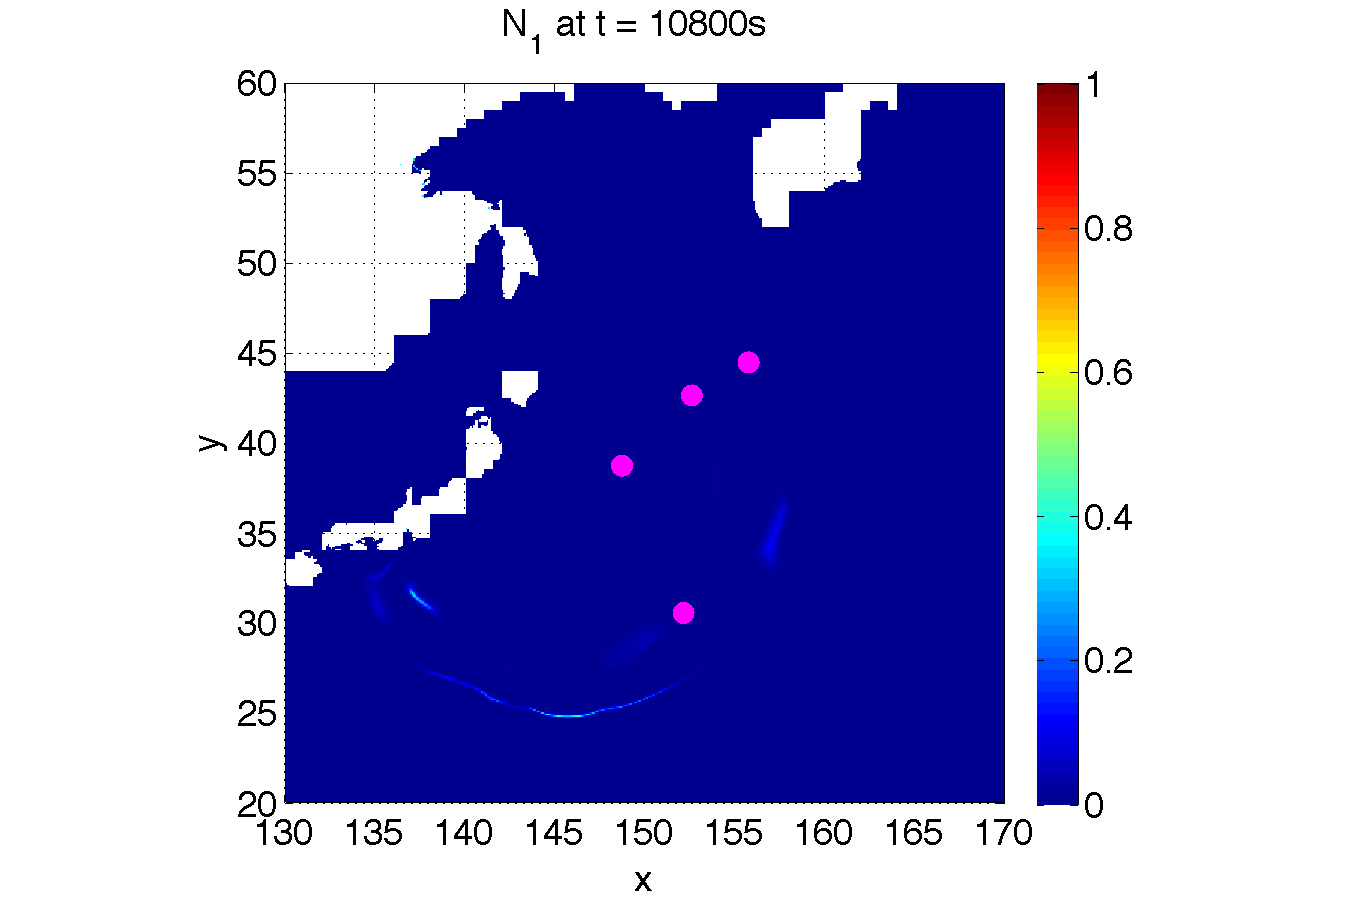
\includegraphics[width=0.45\textwidth]{./figures/T12d3.pdf} &
\hspace*{-45pt}
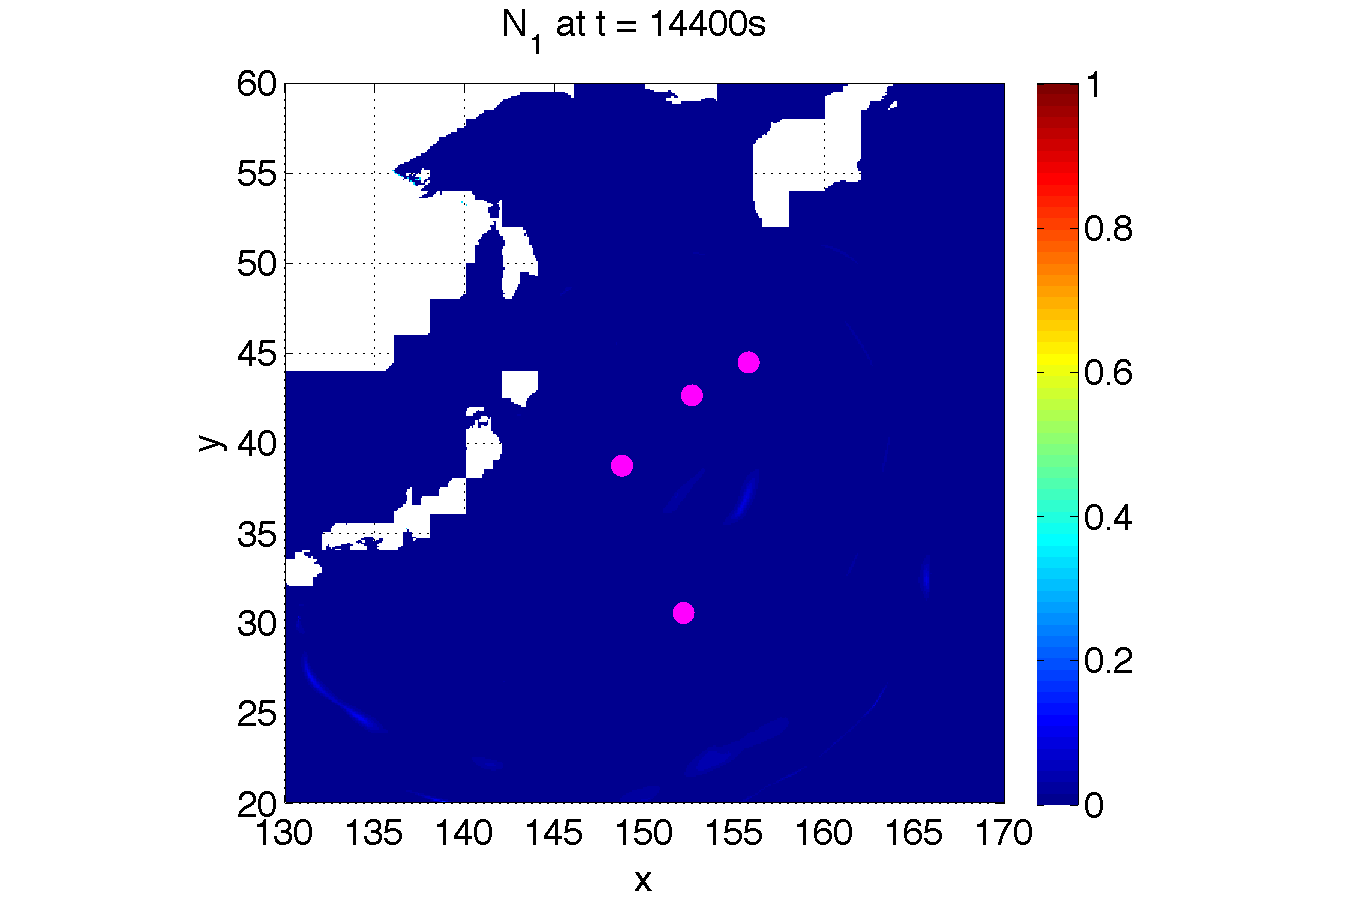
\includegraphics[width=0.45\textwidth]{./figures/T12d4.pdf} \\
\hspace*{-55pt}
\includegraphics[width=0.45\textwidth]{./figures/T22d1.pdf} &
\hspace*{-45pt}
\includegraphics[width=0.45\textwidth]{./figures/T22d3.pdf} &
\hspace*{-45pt}
\includegraphics[width=0.45\textwidth]{./figures/T22d4.pdf} \\
\hspace*{-55pt}
\includegraphics[width=0.45\textwidth]{./figures/T32d1.pdf} &
\hspace*{-45pt}
\includegraphics[width=0.45\textwidth]{./figures/T32d3.pdf} &
\hspace*{-45pt}
\includegraphics[width=0.45\textwidth]{./figures/T32d4.pdf}
\end{tabular}
\caption{Total sensitivity index for $n_1$ (top row) $n_2$ (center row) and $n_3$ (bottom row)
 at different times as indicated.}
\label{fig:sens2d}
\end{figure}
%%%%%%%%%%%%%%%%%%%%%%%%%%%%%%%%%%%%%%%%%%%%%%%%%%%%%%%%%%%%%%%%
\begin{figure}[ht]
\centering

\begin{tabular}{clcl}
\includegraphics[width=0.5\textwidth]{./figures/response_i1_t2.pdf} &
\includegraphics[width=0.5\textwidth]{./figures/response_i2_t2.pdf} \\
\includegraphics[width=0.5\textwidth]{./figures/response_i3_t2.pdf} &
\includegraphics[width=0.5\textwidth]{./figures/response_i4_t2.pdf}
\end{tabular}
\caption{Response surface of water surface elevation at the different gauge locations at t = 7200 s
as function of $n_2$ and $n_3$, with fixed $n_1=0.035$}.
\label{fig:response2}
\end{figure}
%%%%%%%%%%%%%%%%%%%%%%%%%%%%%%%%%%%%%%%%%%%%%%%%%%%%%%%%%%%%%%%%
%\begin{figure}[ht]
%\centering
%
%\begin{tabular}{clcl}
%\includegraphics[width=0.5\textwidth]{./figures/response_i1_t3.pdf} &
%\includegraphics[width=0.5\textwidth]{./figures/response_i2_t3.pdf} \\
%\includegraphics[width=0.5\textwidth]{./figures/response_i3_t3.pdf} &
%\includegraphics[width=0.5\textwidth]{./figures/response_i4_t3.pdf}
%\end{tabular}
%\caption{Response surface of water surface elevation at the different gauge locations at t = 14400 s.}
%\label{fig:response3}
%\end{figure}
%%%%%%%%%%%%%%%%%%%%%%%%%%%%%%%%%%%%%%%%%%%%%%%%%%%%%%%%%%%%%%%%
\begin{figure}[ht]
\centering
\includegraphics[width=0.575\textwidth]{./figures/scatter.pdf} 
\caption{Scatter plot of measured water surface elevation against their \geoclaw
model counterparts during Tsunami \tohoku. The data points are colored 
differently for the different gauges as indicated in the legend. }
\label{fig:scatter}

\end{figure}  
%%%%%%%%%%%%%%%%%%%%%%%%%%%%%%%%%%%%%%%%%%%%%%%%%%%%%%%%%%%%%%%%
\begin{figure}[ht]
\begin{tabular}{clc}
\includegraphics[width=0.475\textwidth]{./figures/chain_p1.pdf} &
\includegraphics[width=0.475\textwidth]{./figures/chain_p2.pdf} \\
\includegraphics[width=0.475\textwidth]{./figures/chain_p3.pdf} &
\includegraphics[width=0.475\textwidth]{./figures/chain_s1.pdf}
\end{tabular}
\caption{Chain samples for the three Manning's $n$ coefficients $n_1,n_2,n_3$ and $\sigma^2$
the variance between simulations and observations. The vertical dotted lines corresponds to the
burn-in iterations.}
\label{fig:mcmc} 
\end{figure}
%%%%%%%%%%%%%%%%%%%%%%%%%%%%%%%%%%%%%%%%%%%%%%%%%%%%%%%%%%%%%%%%
 \begin{figure}[ht]
        \begin{tabular}{clc}
\includegraphics[width=0.475\textwidth]{./figures/pdf_p1.pdf} &
\includegraphics[width=0.475\textwidth]{./figures/pdf_p2.pdf} \\
\includegraphics[width=0.475\textwidth]{./figures/pdf_p3.pdf} &
\includegraphics[width=0.475\textwidth]{./figures/pdf_s1.pdf}
        \end{tabular}
        \caption{KDE of the marginalized posterior distributions for the three Manning's $n$ coefficients $n_1,n_2,n_3$ 
and $\sigma^2$ the variance between simulations and observations.}
\label{fig:pdfs} 
        \end{figure}
%%%%%%%%%%%%%%%%%%%%%%%%%%%%%%%%%%%%%%%%%%%%%%%%%%%%%%%%%%%%%%%%
 \begin{figure}[ht]
        \begin{tabular}{clc}
\includegraphics[width=0.475\textwidth]{./figures/sample12.pdf} &
\includegraphics[width=0.475\textwidth]{./figures/jpdf12.pdf} \\
\includegraphics[width=0.475\textwidth]{./figures/sample13.pdf} &
\includegraphics[width=0.475\textwidth]{./figures/jpdf13.pdf} \\
\includegraphics[width=0.475\textwidth]{./figures/sample23.pdf} &
\includegraphics[width=0.475\textwidth]{./figures/jpdf23.pdf}
        \end{tabular}
\caption{Left: scatter plots of the pairs $(n_1,n_2)$,$(n_1,n_3)$ and $(n_2,n_3)$ obtained from the
chain samples (Figure~\ref{fig:mcmc}). 
Right: contour plots of the marginalized joint posterior distribution of $(n_1,n_2)$,$(n_1,n_3)$ and $(n_2,n_3)$.  Contours of greater than $10\%$ of the maximum probability are shown.}
\label{fig:joint} 
        \end{figure}
%%%%%%%%%%%%%%%%%%%%%%%%%%%%%%%%%%%%%%%%%%%%%%%%%%%%%%%%%%%%%%%%
%  \begin{figure}[ht]
%         \begin{tabular}{clc}
% \includegraphics[width=0.475\textwidth]{./figures/2sample12.pdf} &
% \includegraphics[width=0.475\textwidth]{./figures/2jpdf12.pdf} \\
% \includegraphics[width=0.475\textwidth]{./figures/2sample13.pdf} &
% \includegraphics[width=0.475\textwidth]{./figures/2jpdf13.pdf} \\
% \includegraphics[width=0.475\textwidth]{./figures/2sample23.pdf} &
% \includegraphics[width=0.475\textwidth]{./figures/2jpdf23.pdf}
%         \end{tabular}
% \caption{\comment{This is for the case of second (Saito) source model} Left: scatter plots of the pairs $(n_1,n_2)$,$(n_1,n_3)$ and $(n_2,n_3)$ obtained from the
% chain samples (Figure~\ref{fig:mcmc}). 
% Right: contour plots of the marginalized joint posterior distribution of $(n_1,n_2)$,$(n_1,n_3)$ and $(n_2,n_3)$.  Contours of greater than $10\%$ of the maximum probability are shown.}
% \label{fig:joint} 
%         \end{figure} 

\clearpage
\bibliographystyle{elsarticle-num}
\bibliography{biblio}
\end{document}
